% presentation template for Applied Numerical Analysis M15, Departement of Mathematics, TUM
%
% Bongini Mattia (Decemeber 2013)

\documentclass[leqno]{beamer}
\setbeamercovered{transparent}
\usetheme[
	showofpages=true, % show total number of pages on each slide
	pageofpages=of,% String used between the current page and the total page count (do not use '/').
	alternativetitlepage=true,% Use the fancy title page.
	headerlogo=logos/newlogo.png,%TUM_LS_M15_OS_CMYK.pdf,% Logo for the first page.
	titleline=true, % show a line below the frame title
	shownavigationsymbols=false, % show the navigation symbols on the bottom left
	bullet = square % square, circle
          ]{m15tum}
          
%\usepackage{multimedia}
%\usepackage{media9}
\usepackage{movie15}
\usepackage{ragged2e}
\usepackage{verbatim}
\usepackage{xmpmulti}
\usepackage{epstopdf}
\usepackage[latin1]{inputenc}
\usepackage{colortbl}
\usepackage[english]{babel}

\usepackage{graphicx}
\usepackage{latexsym}
\usepackage{xcolor}
\usepackage{amssymb}
\usepackage{amscd}
\usepackage{mathrsfs}
\usepackage{amsmath}
\usepackage{amsfonts}
\usepackage{amsthm}
\usepackage{mdframed}


\makeatletter
\renewcommand{\itemize}[1][]{%
  \beamer@ifempty{#1}{}{\def\beamer@defaultospec{#1}}%
  \ifnum \@itemdepth >2\relax\@toodeep\else
    \advance\@itemdepth\@ne
    \beamer@computepref\@itemdepth% sets \beameritemnestingprefix
    \usebeamerfont{itemize/enumerate \beameritemnestingprefix body}%
    \usebeamercolor[fg]{itemize/enumerate \beameritemnestingprefix body}%
    \usebeamertemplate{itemize/enumerate \beameritemnestingprefix body begin}%
    \list
      {\usebeamertemplate{itemize \beameritemnestingprefix item}}
      {\def\makelabel##1{%
          {%
            \hss\llap{{%
                \usebeamerfont*{itemize \beameritemnestingprefix item}%
                \usebeamercolor[fg]{itemize \beameritemnestingprefix item}##1}}%
          }%
        }%
      }
  \fi%
  \beamer@cramped%
  \justifying% NEW
  %\raggedright% ORIGINAL
  \beamer@firstlineitemizeunskip%
}
\makeatother

\usefonttheme{serif}


% user declarations

\newcommand{\ph}{\varphi}
\newcommand{\Om}{\Omega}
\newcommand{\lj}{_{\ell}^j}
\newcommand{\eps}{\varepsilon}
\newcommand{\contradiction}{{\hbox{%
    \setbox0=\hbox{$\mkern-3mu\times\mkern-3mu$}%
    \setbox1=\hbox to0pt{\hss$\times$\hss}%
    \copy0\raisebox{0.5\wd0}{\copy1}\raisebox{-0.5\wd0}{\box1}\box0
}}}

\newcommand{\R}{\mathbb{R}}
\newcommand{\N}{\mathbb{N}}
\newcommand{\C}{\mathbb{C}}
\newcommand{\Z}{\mathbb{Z}}
\newcommand{\hyp}{\R^n \setminus \R^{\ell}}

\newcommand{\Ad}{A}
\newcommand{\Adcut}{S}
\newcommand{\At}{A^{\textsc{targ}}}
\newcommand{\Crand}{C^{\textsc{z}}}
\newcommand{\Cchar}{C^{\textsc{v}}}
\newcommand{\Cr}{C_{\textsc{F}}^{\textsc{r}}}
\newcommand{\Crl}{C_{\textsc{L}}^{\textsc{r}}}
\newcommand{\Ct}{C^{\textsc{d}}}
\newcommand{\Ca}{C^{\textsc{a}}}
\newcommand{\HFF}{H^{\textsc{F}}}
\newcommand{\HFL}{H^{\textsc{L}}}
\newcommand{\HLF}{K^{\textsc{F}}}
\newcommand{\HLL}{K^{\textsc{L}}}
\newcommand{\NF}{N^{\textsc{F}}}
\newcommand{\NL}{N^{\textsc{L}}}
\newcommand{\rhoF}{\rho^{\textsc{F}}}
\newcommand{\rhoL}{\rho^{\textsc{L}}}
\newcommand{\etaF}{\eta^{\textsc{F}}}
\newcommand{\etaL}{\eta^{\textsc{L}}}
\newcommand{\lamF}{\lambda^{\textsc{F}}}
\newcommand{\lamL}{\lambda^{\textsc{L}}}
\newcommand{\thetaF}{\vartheta^{\textsc{F}}}
\newcommand{\thetaL}{\vartheta^{\textsc{L}}}
\newcommand{\RestF}{\Xi_{\varphi}^{\textsc{F}}}
\newcommand{\RestL}{\Xi_{\varphi}^{\textsc{L}}}
\newcommand{\noisepar}{\Crand}
%\newcommand{\xf}{x^{\textsc{f}}}
%\newcommand{\xl}{x^{\textsc{l}}}
%\newcommand{\vf}{v^{\textsc{f}}}
%\newcommand{\vl}{v^{\textsc{l}}}
\newcommand{\xf}{x}
\newcommand{\xl}{y}
\newcommand{\vf}{v}
\newcommand{\vl}{w}
\newcommand{\target}{x^\textsc{d}}
\newcommand{\CclosenessLF}{C^{\textsc{L}}}
\newcommand{\CclosenessFF}{C^{\textsc{F}}}
\newcommand{\Ccongestion}{C^{\textsc{cong}}}
\newcommand{\Ccontrol}{\nu}


\DeclareMathOperator*{\argmin}{\arg\!\min}
\DeclareMathOperator{\tr}{tr}
\DeclareMathOperator{\Ext}{Ext}
\DeclareMathOperator{\dist}{dist}
\DeclareMathOperator{\rinf}{rinf}
\DeclareMathOperator{\supp}{supp}

\newtheorem{maintheorem}[theorem]{Main Theorem}
\newtheorem{proposition}[theorem]{Proposition}
\newtheorem{defn}[theorem]{Definition}

\def\nnew{\color{red}}
\def\bnew{\color{blue}}

\definecolor{forestgreen}{rgb}{0.13, 0.55, 0.13}
\definecolor{goldenrod}{rgb}{0.85, 0.65, 0.13}

% title page declarations
\author[M. Bongini]{Mattia Bongini}
\title[Inferring Interaction Rules from Observations of Evolutive Systems]{\fontsize{19}{26}\selectfont Inferring Interaction Rules from \quad\quad\quad\quad\quad\quad\quad\quad\quad\quad\quad\quad Observations of Evolutive Systems\vspace{0.3cm} \quad\quad\quad\quad\quad\quad\quad\quad\quad\quad\quad\quad\quad\quad \small (joint work with M. Fornasier, M. Hansen and M. Maggioni)}
\institute{Technische Universit\"at M\"unchen, \\ Department of Mathematics, \\ Chair of Applied Numerical Analysis \\ ~ \\ bongini@ma.tum.de\\ ~ \\Data-Rich Phenomena\\Cambridge\\ December 14-16, 2015}
%\date{Mathematical Control in Trieste, Cambridge, December 14-16, 2015}



% Add toc before each section
\AtBeginSection[]
{
  \begin{frame}
    \frametitle{Overview}
    \tableofcontents[currentsection]
  \end{frame}
}

\begin{document}
%\include{presentation_m15_template_content}


\frame{\titlepage}

%\frame{
%\frametitle{Complex networks in everyday life}
%Large self-organizing interconnected systems arise everywhere:
%\begin{columns}
%\begin{column}{6cm}
%\begin{center}
%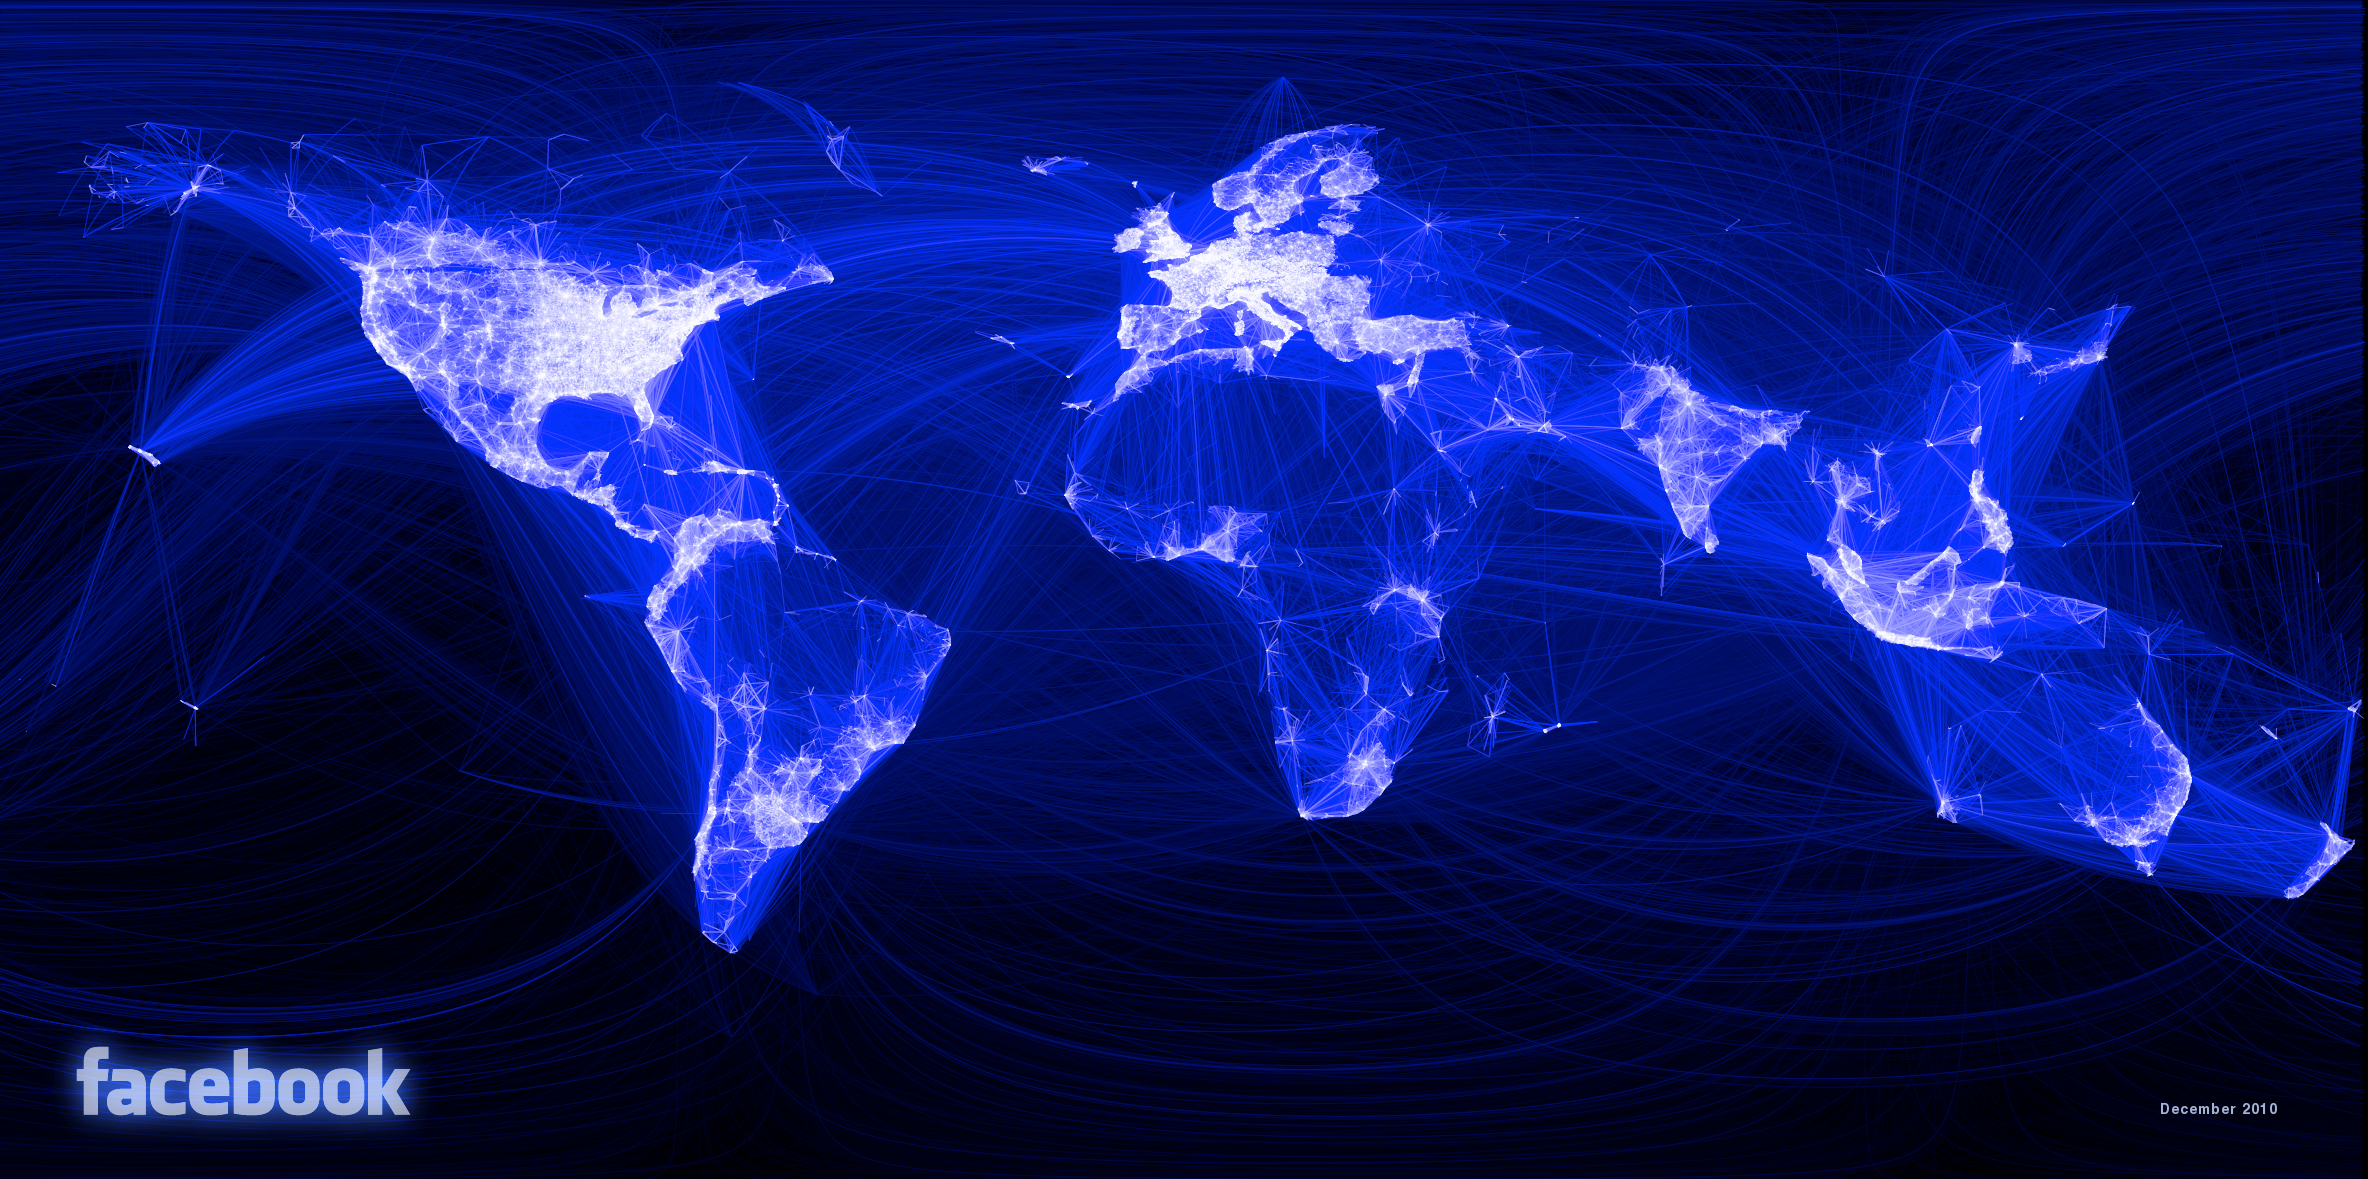
\includegraphics[width=4cm]{images/facebook_connections.png}\\
%{\it  \scriptsize Facebook  ``friendship'' network}
%\end{center}
%\begin{center}
%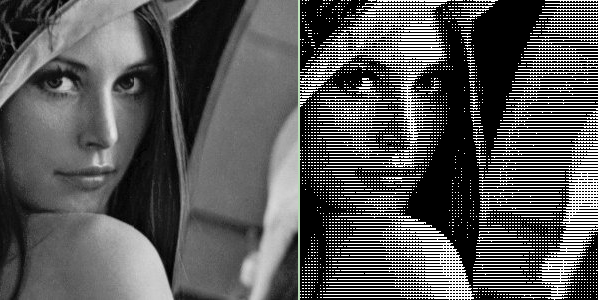
\includegraphics[width=4cm]{images/dither1.png}\\
%{\it \scriptsize Image halftoning}
%\end{center}
%\end{column}
%
%\begin{column}{6cm}
%\begin{center}
%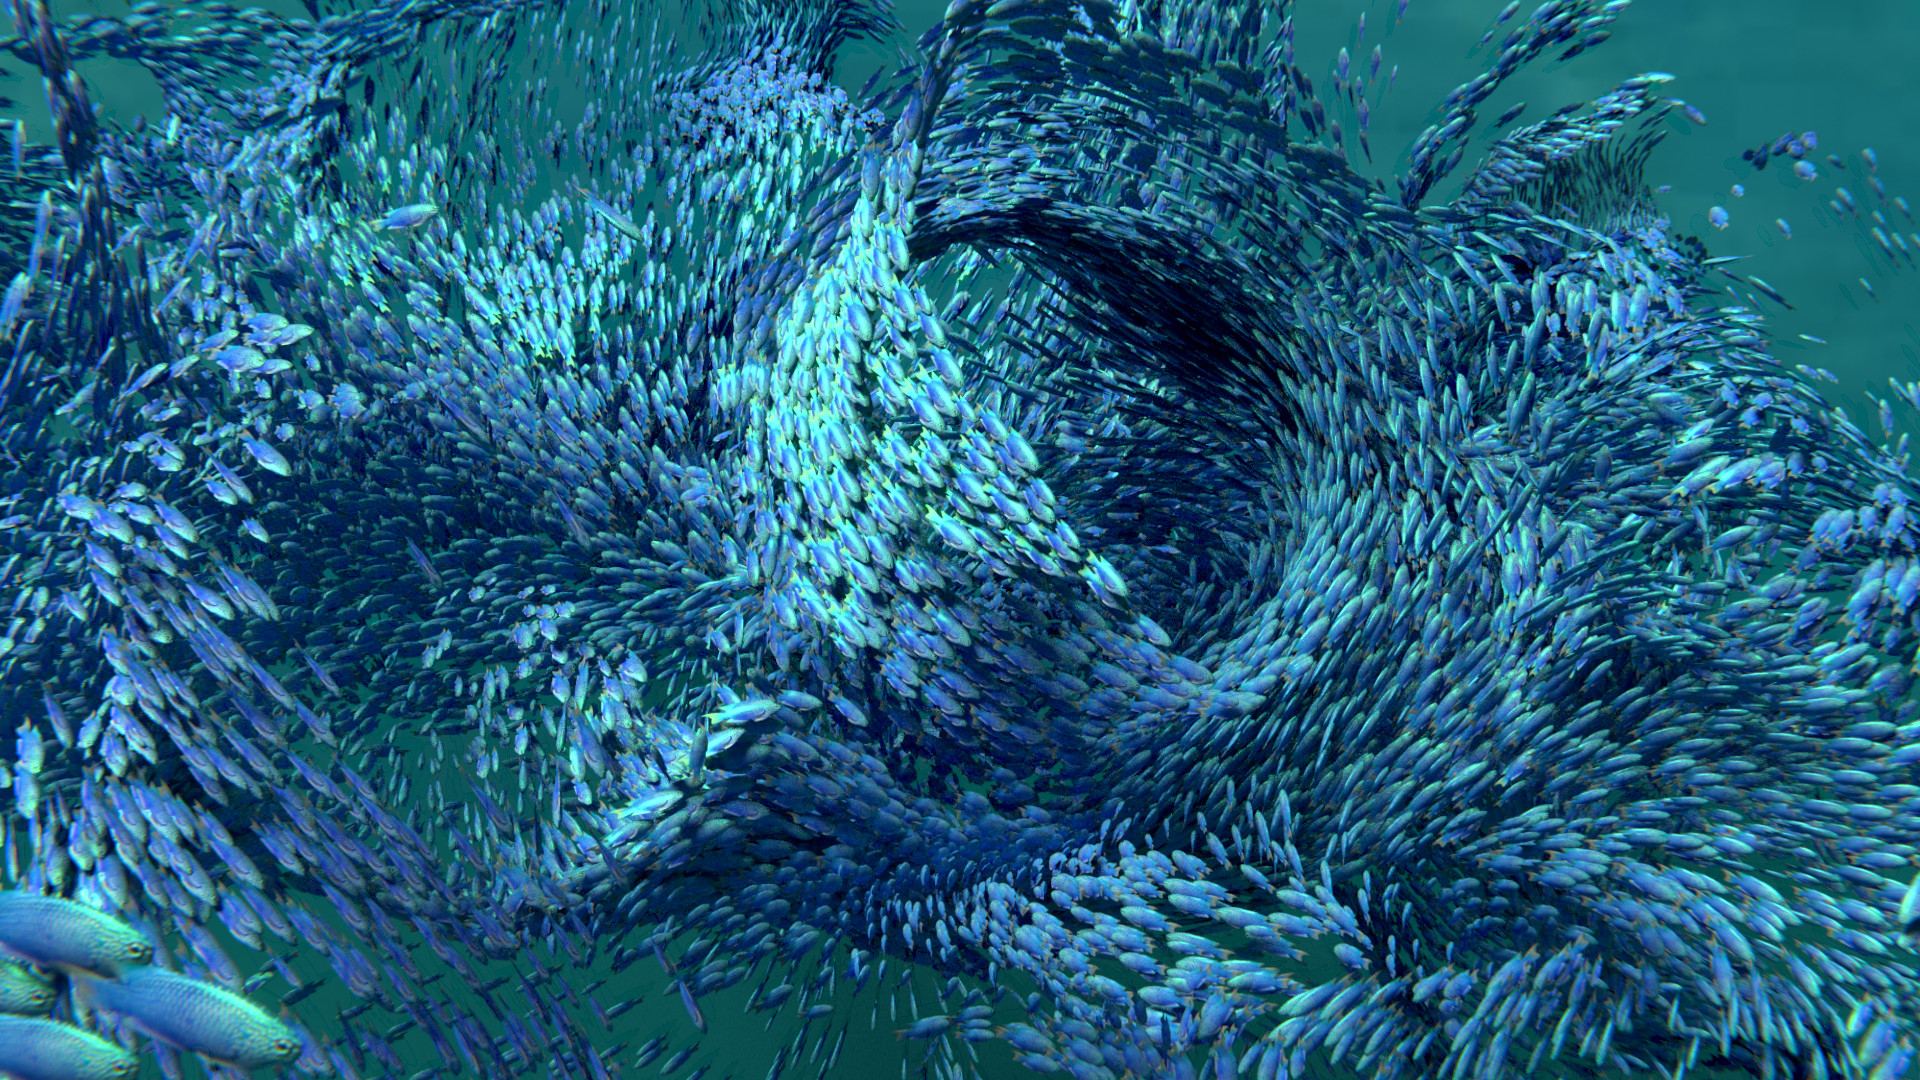
\includegraphics[width=4cm]{images/Fish_Final.jpg}\\
%{\it  \scriptsize Schools of fishes}
%\end{center}
%\begin{center}
%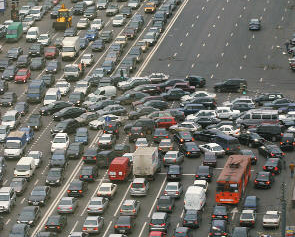
\includegraphics[width=3cm]{images/j.png}\\
%{\it  \scriptsize Traffic jams}
%\end{center}
%\end{column}
%\end{columns}}


%\frame{
%\frametitle{What is a self-organizing system?}
%\begin{center}
%\vskip -.1cm
%%\movie[width=5cm,height=5cm,poster]{}{fish.mp4}
%%%&
%%\movie[width=5cm,height=5cm,poster]{}{flock.mp4}
%\movie[width=4.25cm,height=3.25cm,poster,autostart,loop]{}{videos/Gretna.mp4}
%%&
%\movie[width=4.25cm,height=3.25cm,poster,autostart,loop]{}{videos/Hajj_s1.mov}
%\\
%\movie[width=4.25cm,height=3.25cm,poster,autostart,loop]{}{videos/Indian.mov}
%%&
%\movie[width=4.25cm,height=3.25cm,autostart,loop]{}{videos/fish.mp4}
%\end{center}
%%\footnotesize\emph{ The whole is greater then the sums of the parts}, Aristoteles, 383 -- 322 B.C.
%}

\frame{
\frametitle{What is a self-organizing system?}
\begin{center}
\vskip -.1cm
%\movie[width=4.25cm,height=3.25cm,poster,autostart,loop]{}{videos/Gretna.mp4}
%\movie[width=4.25cm,height=3.25cm,poster,autostart,loop]{}{videos/Hajj_s1.mov}
%\\
%\movie[width=4.25cm,height=3.25cm,poster,autostart,loop]{}{videos/Indian.mov}
%\movie[width=4.25cm,height=3.25cm,autostart,loop]{}{videos/fish.mp4}
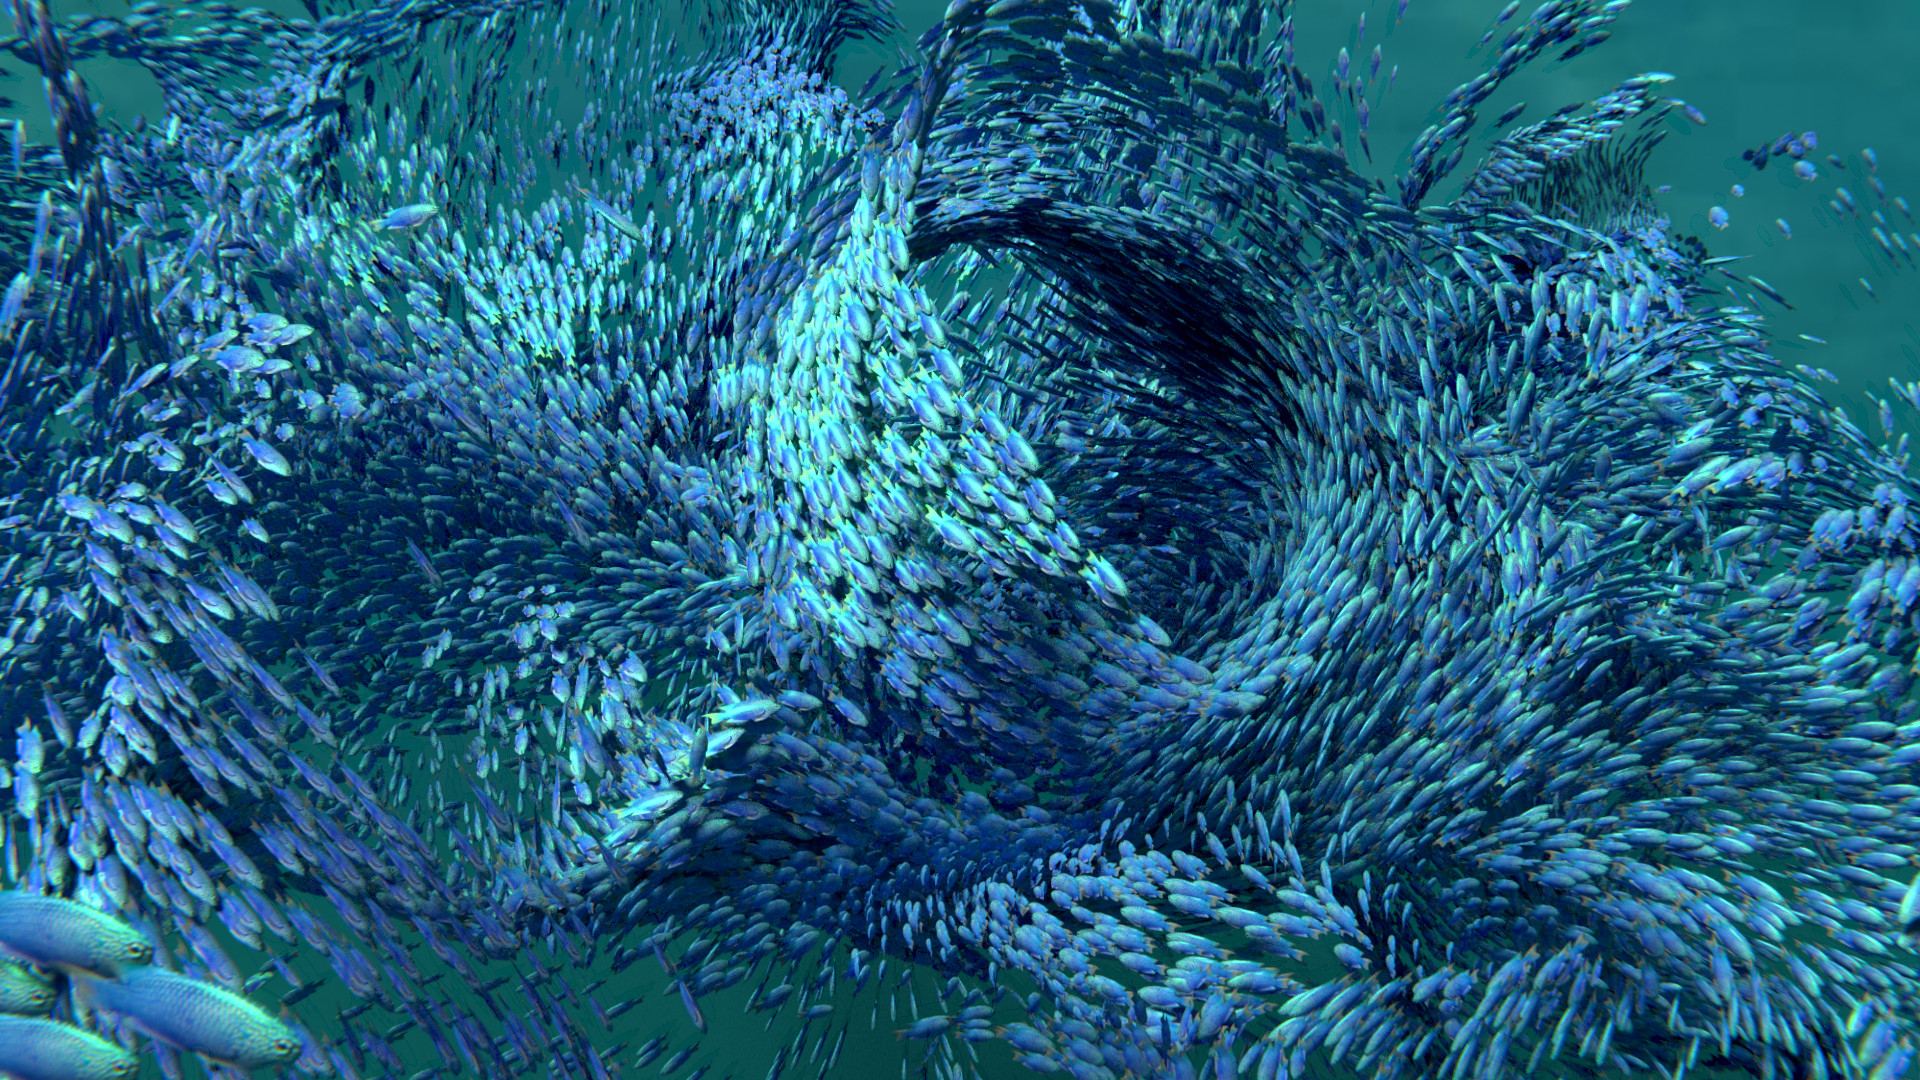
\includegraphics[width=4.8cm,height=3.2cm]{images/Fish_Final.jpg}\;
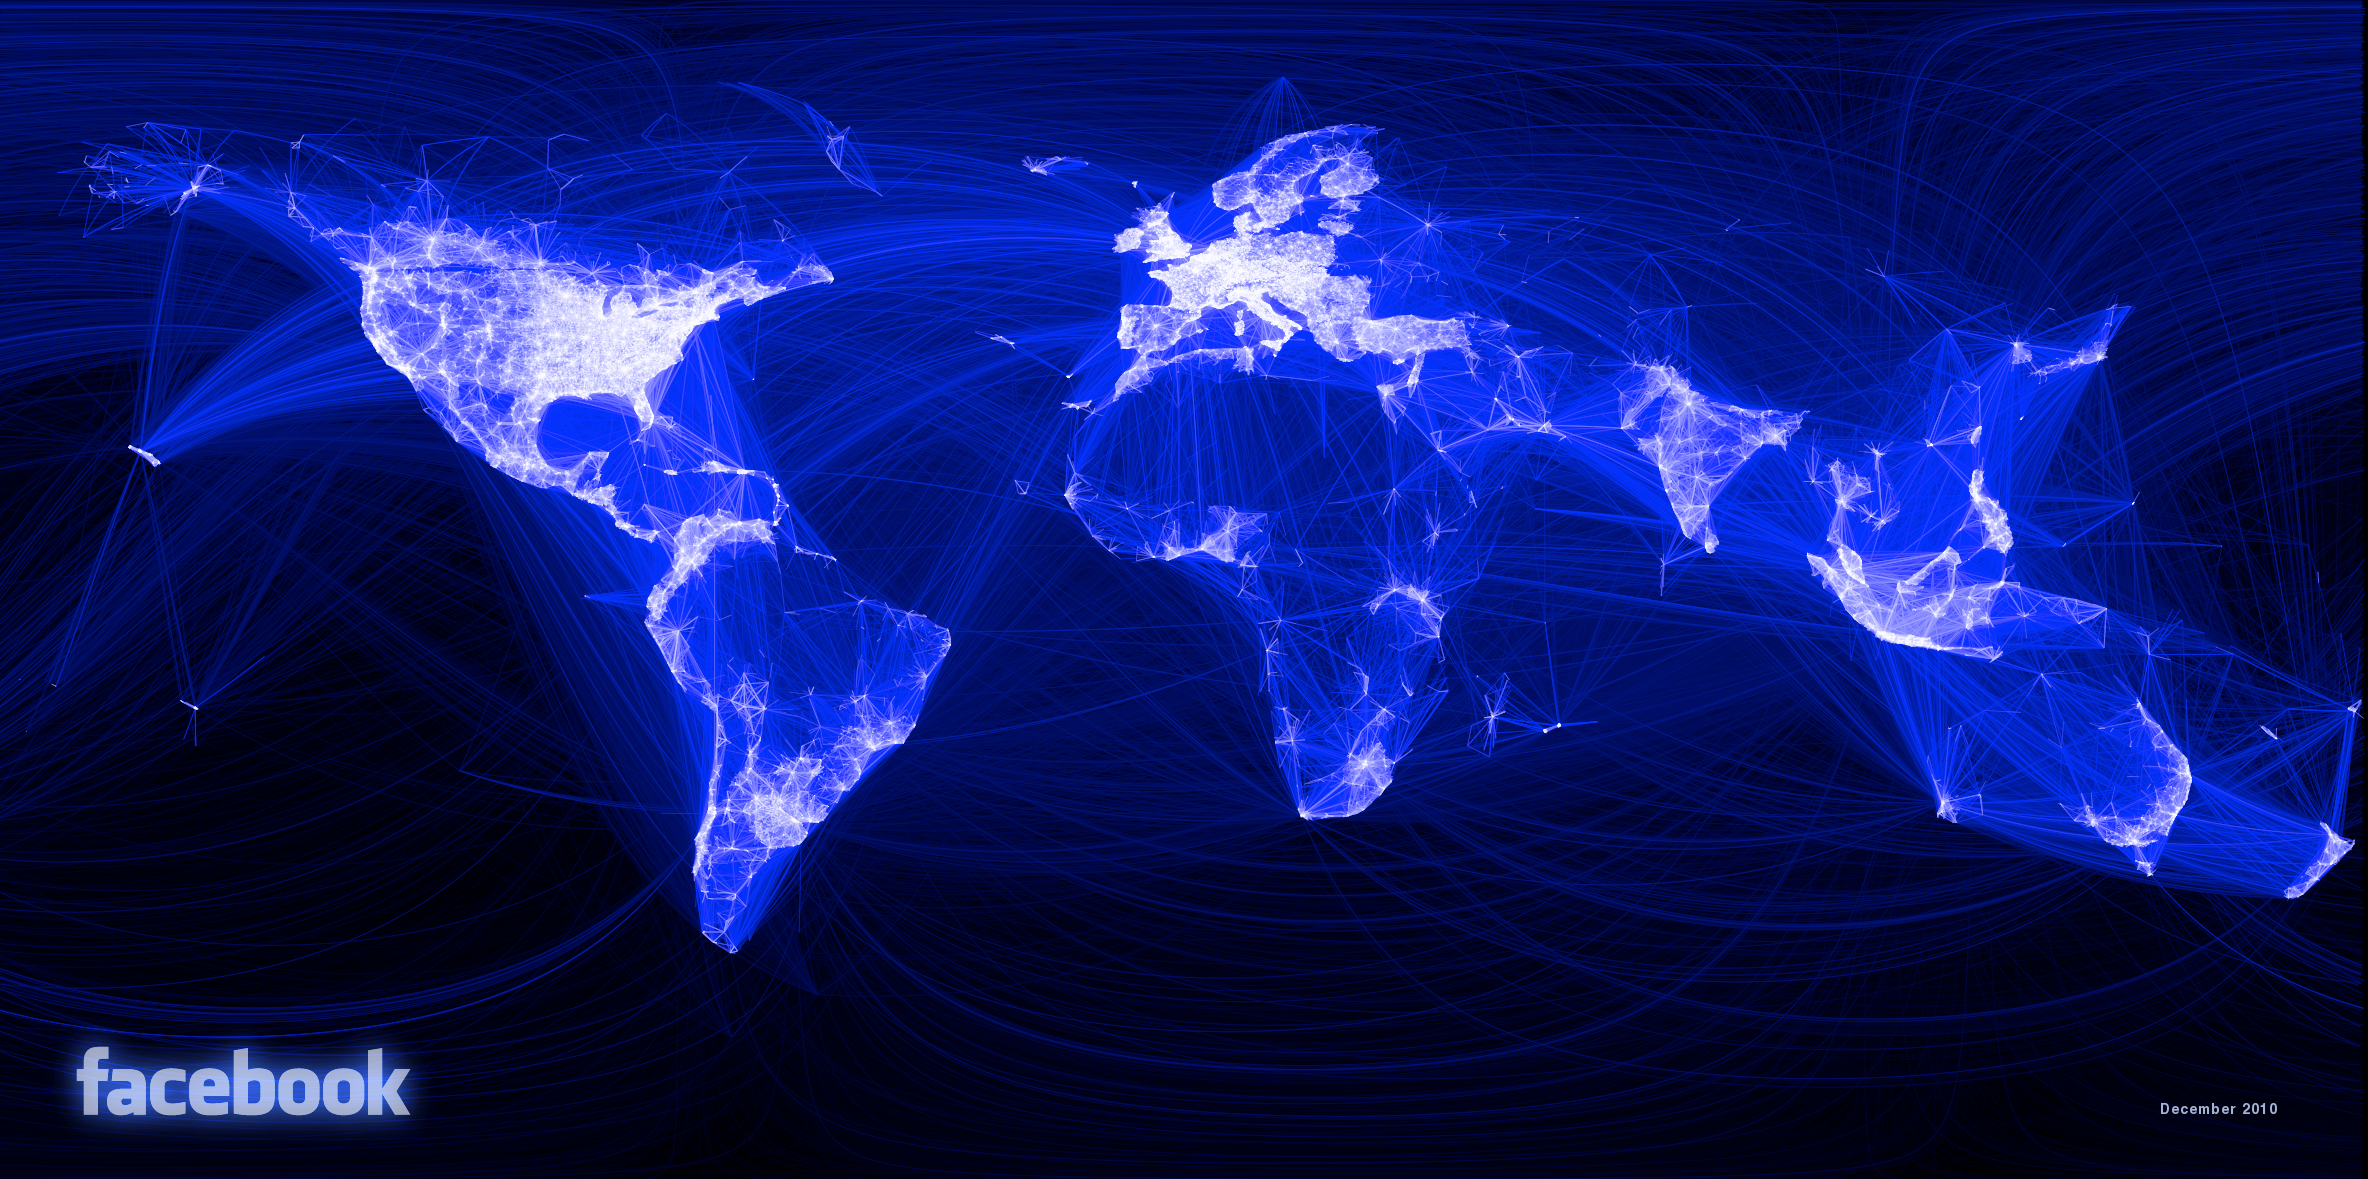
\includegraphics[width=4.8cm,height=3.2cm]{images/facebook_connections.png}\\
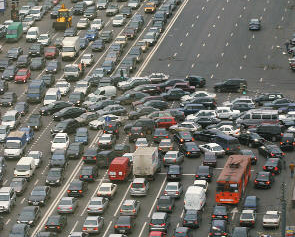
\includegraphics[width=4.8cm,height=3.2cm]{images/j.png}\;
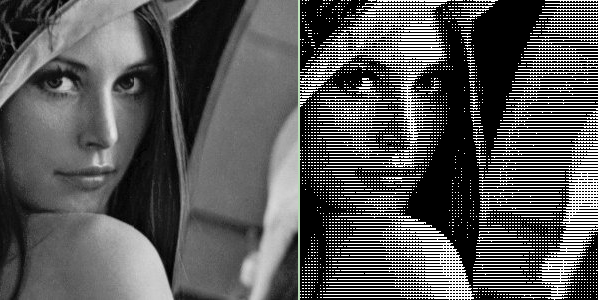
\includegraphics[width=4.8cm,height=3.2cm]{images/dither1.png}
\end{center}
}

\frame{
\frametitle{A framework for social dynamics}
\justifying
\begin{columns}
\begin{column}{5.5cm}
\justifying
We consider multiagent systems of the form: for $i=1,\dots, N$
{\color{blue}$$
\dot x_i = \frac{1}{N}\sum^N_{j = 1}a(|x_i - x_j|)(x_j - x_i) \in \R^d,
$$}and their mean-field limit equation (here $F[a](\xi) = -a(|\xi|)\xi$)
{\color{blue}$$
\frac{\partial \mu}{\partial t} = -\nabla\cdot((F[a]*\mu)\mu),
$$}
\end{column}
\begin{column}{5.5cm}
\begin{center}
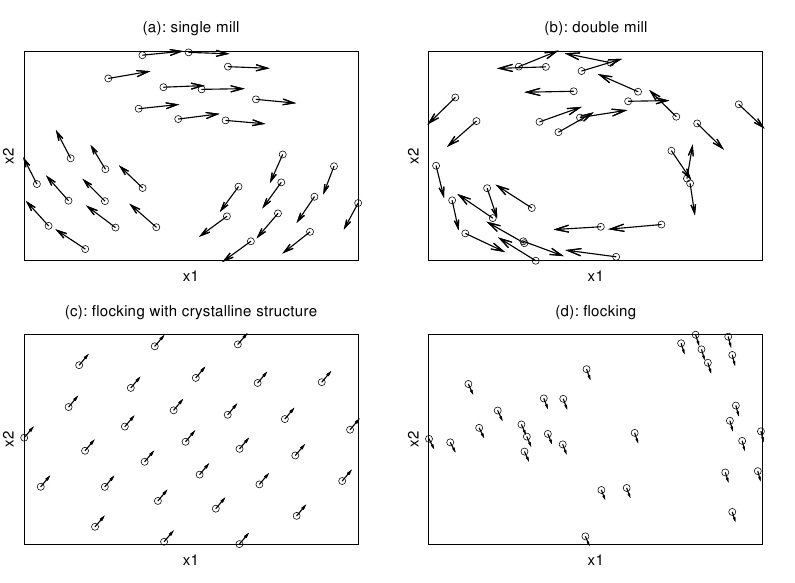
\includegraphics[width=5.3cm,height=4.3cm]{images/consensusImage.jpg}\\
%\movie[width=2.5cm,height=2cm,autostart,loop]{}{videos/clust_a5_b15.mov}
%\movie[width=2.5cm,height=2cm,autostart,loop]{}{videos/clust_a5_b25.mov}\\
%\movie[width=2.5cm,height=2cm,autostart,loop]{}{videos/Mill2Flock.mov}
%\movie[width=2.5cm,height=2cm,autostart,loop]{}{videos/Rand2Mill.mov}\\
{\it \scriptsize Patterns related to different \\balances of social forces}
\end{center}
\end{column}
\end{columns}
\vspace{0.1cm}
\pause
Several ``social forces'' encoded in the {\color{red}interaction kernel $a$}:
\begin{itemize}
\item alignment;
\item repulsion-attraction;
\item self-propulsion/friction...
\end{itemize}
%\pause
%\vskip0.2cm
%{\color{red} Understanding how superposition of re-iterated binary ``social forces'' yields global self-organization}
}

\frame{
\frametitle{The problem}
\vspace{-0.2cm}
\begin{itemize}
\justifying
\item Tremendous theoretical success but the issue of actual applicability is so far scarcely addressed;
\pause
\item Purely {\color{blue} qualitative analysis} to reproduce macroscopical patterns;
\pause
\item Well-posedness relies on smoothness and asymptotic properties of the kernel $a$ at $0$ and $\infty$;
\pause
\item Certainly  results  of great importance, as such  functions  likely  differ  from  physical models: it is legitimate to consider a {\color{blue}large variety of function classes};
\pause
\item However, a solid mathematical framework on `learnability" of interactions from observations of the dynamics {\color{blue}is not yet available}.
\end{itemize}
\pause
\begin{columns}
\visible<6->{\begin{column}{4.5cm}
%\movie[width=4.25cm,height=3.25cm,poster,autostart,loop]{}{videos/Hajj_s1.mov}
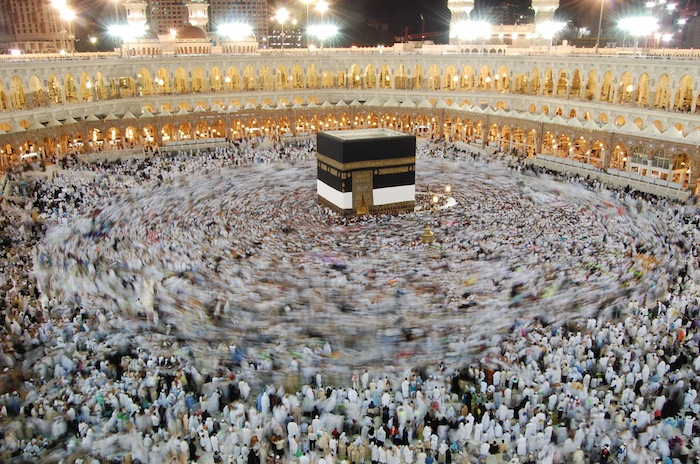
\includegraphics[width=4.2cm,height=2.6cm]{images/sinner.jpg}
\end{column}
\begin{column}{7cm}
$$\!\!\!\! \Rightarrow \;\; a(r) = \sin\left(\log(r+1)\prod_{i = 1}^d e^{\cos(i \cdot r^2)} + \ldots\right)$$
\end{column}
\end{columns}}
}

\frame{
\frametitle{The {\it naive} approach: optimal control}
\justifying
Given a {\color{blue}finite time horizon $T > 0$} one would seek for a minimizer $\widehat a$ of
\begin{align*}
\mathcal E(\widehat a) = \frac{1}{T}\int_0^T \left [ \|x[a](s) - x[\widehat a](s)\|^2 + \mathcal R(\widehat a) \right ] d s ,
\end{align*}
being $\mathcal{R}$ a suitable regularization functional and $t \mapsto x[\widehat a](t) = (x_1(t),\ldots,x_N(t))$ be the solution of
$$
\dot x_i = \frac{1}{N}\sum^N_{j = 1}\widehat a(|x_i - x_j|)(x_j - x_i).
$$
\pause
{\color{red}However, one faces several problems!}
\pause
\begin{itemize}
\item $t \mapsto x[\widehat a](t)$ strongly nonlinear $\Rightarrow$ $\mathcal E(\widehat a)$ strongly nonconvex; \pause
\item computationally unfeasible for $N$ large (curse of dimensionality -  Richard E. Bellman).
\end{itemize}
}

\frame{
\frametitle{The variational approach}
\justifying
Instead of minimizing the distances between trajectories $x[\widehat a](t)$, we minimize the discrepancy between velocities $\dot{x}_i(t)$,
\small{
\begin{align*}
	\mathcal E_N(\widehat a) = \frac{1}{T}\int_0^T\frac{1}{N}\sum_{i=1}^N\biggl|{\color{red}\frac{1}{N}\sum_{j=1}^N\widehat a(|x_i(t)-x_j(t)|)(x_i(t) - x_j(t))}-\dot{x}_i(t)\biggr|^2 dt,
\end{align*}}
\pause
among all functions
{\color{blue}$$\widehat a \in X=\bigl\{b:\R_+\rightarrow\R\,|\ b \in L_{\infty}(\R_+) \cap W^{1}_{\infty,loc}(\R_+) \bigr \}$$}
{\color{red}(ODEs and mean-field equations are well-posed)}.
\pause
%\vspace{-0.5cm}
\begin{proposition}
\justifying
If $a,\widehat a \in X$ then there exist a constant $C>0$ depending on $T,\widehat a$ and $x_{0,1},\ldots,x_{0,N}$ and a ``certain'' compact set $K \subset \R_+$ such that
\begin{equation*}
\| x[a](t) -x[\widehat a](t) \| \leq C \sqrt{\mathcal E_N(\widehat a)} \quad \text{ for all } t \in [0,T].
\end{equation*}
Hence, {\color{blue}minimizing $\mathcal E_N(\widehat a)$ implies an accurate approximation of $t \mapsto x[\widehat a](t)$ at finite time.} (Proof: just a Gronwall.)
\end{proposition}
}

\frame{
\frametitle{The main question}
\begin{itemize}
\justifying
\item $\mathcal E_N$ is easily computable from the knowledge of the trajectories of the system $x[a](t)$ (perhaps approximating $\dot{x}_i(t)$ by $\frac{x_i(t+\delta t) - x_i(t)}{\delta t}$).
\pause
\item We use the number of agents $N$ as an {\color{red}optimization parameter}: does a larger number of agents improve learnability?
\pause
\item Being quadratic (its minimization is just a least squares!!!), its minimizers can be {\color{red}efficiently numerically computed} on a finite dimensional space $V_N \subset X$ such that $V_N \nearrow X$ as $N\rightarrow +\infty$.
\end{itemize}
\pause
\begin{center}
\begin{mdframed}
{\color{blue}Question: for which sequence $V_N$ do minimizers
\begin{align*}
\widehat a_{N} \in \argmin_{\widehat a \in V_N} \mathcal E_N(\widehat a)
\end{align*}
satisfy $\widehat a_{N} \rightarrow a$, and in which topology does this limit hold?}
\end{mdframed}
\end{center}
}

\frame{
\frametitle{$\Gamma$-limit of the $\mathcal E_N$}
\begin{itemize}
\justifying
\item Suppose there exists a functional $\mathcal E$ such that {\color{red}$a = \argmin_{\widehat a \in X} \mathcal E(\widehat a)$}.
\pause
\item Then the above question translates into the convergence of the minimizers of $\mathcal E_N$ to the minimizer of $\mathcal E$, i.e., the {\color{blue}$\Gamma$-convergence of $\mathcal E_N$ to $\mathcal E$}. \pause {\color{red}But what can  $\mathcal E$ be?}
\pause
\item Set $F[a](\xi) = -a(|\xi|)\xi$ and rewrite the initial system as
\begin{align*}
\left\{\begin{aligned}
\dot{x}^N_i(t) &= \frac{1}{N}\sum^N_{j = 1}{\color{blue}F[a]}(x^N_i(t) - x^N_j(t)) \; \text{ for } t \in (0,T],\\
x_i^N(0) &= x^N_{0,i},
\end{aligned} \; i = 1, \ldots, N. \right.
\end{align*}
\pause
\item Define the {\color{blue}empirical measure} $\mu^N:[0,T]\rightarrow\mathcal{P}_c(\R^d)$ as
\begin{align*}
\mu^N(t) = \frac{1}{N}\sum^N_{i = 1} \delta_ {x^N_i(t)}.
\end{align*}
\end{itemize}
}

\frame{
\frametitle{A possible solution: the continuity equation}
\begin{itemize}
\justifying
\item $\mu^N$ is a solution to the {\color{red}continuity equation} (abbreviated {\color{red}c.e.})
{\color{blue}\begin{align*}
\frac{\partial \mu}{\partial t}(t) &= -\nabla \cdot ((F[a]*\mu(t))\mu(t)) \quad \text{ for } t \in (0,T].
\end{align*}}
with initial datum $\mu^N(0) = \mu^N_0 := \frac{1}{N}\sum^N_{i = 1} \delta_ {x^N_{0,i}}$.

\pause
\item Moreover, we can now rewrite $\mathcal E_N$ as
\begin{align*}
	\begin{split}
	\mathcal E_N(\widehat a) & = \frac{1}{T}\int_0^T\frac{1}{N}\sum_{i=1}^N\biggl|\frac{1}{N}\sum_{j=1}^N
			\bigl(F[\widehat a]-F[a]\bigr)(x_i-x_j)\biggr|^2 dt\\ \pause
			& = \frac{1}{T}\int_0^T \int_{\R^d} \biggl|\bigl(F[\widehat a]-F[a]\bigr)\ast{\color{blue}\mu^N}(t)\biggr|^2d{\color{blue}\mu^N}(t)(x)dt,
	\end{split}
\end{align*}
%\pause
%\item Hence the question is: {\color{red}do} and {\color{red}in which sense} the $\mu^N$ converge to something as $N \rightarrow +\infty$?
\end{itemize}
}

\frame{
\frametitle{Existence and uniqueness of solutions of the c.e.}
\vspace{-0.3cm}
\begin{theorem}
\justifying
\vspace{-0.2cm}
\begin{itemize}
\justifying
\item Suppose $a \in X$, let $T > 0$ and fix $\mu_0 \in \mathcal{P}_c(\R^d)$.
\pause
\item Let $\mu$ be a weak solution of the c.e. with $\mu(0) = \mu_0$ on $[0,T]$.
\pause
\item Let $\mu^{N}_0 = \frac{1}{N}\sum^N_{i = 1} \delta_{x^{N}_{0,i}}$ be such that $x^N_{0,i} \sim \mu_0$ i.i.d. $\forall N$ and $\forall i$.
\end{itemize}
\vspace{-0.1cm}
\pause
Then, $\exists R > 0$ depending only on $T,a$, and $\supp(\mu_0)$ such that %up to subsequences
it holds
\pause
{\color{blue}\begin{align*}
\supp(\mu^N(t)) \cup \supp(\mu(t)) \subseteq B(0,R), &\;\forall N \in \N \text{ and } \forall t \in [0,T],
\end{align*}}
\pause
\vspace{-0.7cm}
{\color{red}\begin{align*}
\lim_{N\rightarrow+\infty}\sup_{t \in [0,T]}\mathcal{W}_1(\mu(t),&\mu^{N}(t)) = 0.
\end{align*}}
%\pause
%\vspace{0.1cm}
%Moreover, if $\mu:[0,T]\rightarrow\mathcal{P}_1(\R^d)$ and $\nu:[0,T]\rightarrow\mathcal{P}_1(\R^d)$ are equi-compactly supported solutions of the c.e. with $\mu(0)=\mu_0$ and $\nu(0)=\nu_0$, then $\exists \overline{C} > 0$ depending only on $T$, $a$,  and $R$ such that
%\vspace{-0.15cm}
%{\color{blue}\begin{align*}
%\mathcal{W}_1(\mu(t), \nu(t)) \le \overline{C} \, \mathcal{W}_1(\mu_0, \nu_0) \;\text{ for every } t \in [0, T].
%\end{align*}}
\end{theorem}
}

\frame{
\frametitle{The limit functional $\mathcal E$}
\begin{itemize}
\justifying
\item Natural candidate for the $\Gamma$-limit   $\mathcal E$ of the $\mathcal E_N$: \pause as {\color{blue}$\mu$ is the uniform limit of the $\mu^N$} then we define 
\begin{align*}
	\mathcal E(\widehat a) = \frac{1}{T}\int_0^T \int_{\R^d} \biggl|\bigl(F[\widehat a]-F[a]\bigr)\ast{\color{blue}\mu}(t)\biggr|^2d{\color{blue}\mu}(t)(x)dt.
\end{align*}
\pause
\item Since $\mathcal{E}(\widehat a) \geq 0$ and $\mathcal{E}(a) = 0$, then $a$ minimizes $\mathcal{E}$. {\color{red}Is it unique?}
\pause
\item Given $d(x,y) = |x-y|$, introduce the family of measures
\begin{align*}
\varrho(t)(A) &= (\mu(t) \otimes \mu(t))(d^{-1}(A)), \mbox{ for all } t \in [0,T] \mbox{ and} \\
\rho(A) & = \frac{1}{T}\int^T_0 \int_A s^2 d\varrho(t)(s) dt
\end{align*}
\pause
$\varrho(t)(s)$ tells precisely {\color{blue}how likely is that there are two indexes $i \not = j$ such that $|x_i(t) - x_j(t)| = s$}, \pause while $\rho(s)$ {\color{blue}averages} these likelihoods over the entire time frame $[0,T]$ (weighted by $s^2$).
\pause
\item {\color{red}$\supp(\rho) \subseteq [0,2R]$}.
\end{itemize}
}

\frame{
\frametitle{The coercivity condition}
\vspace{-0.2cm}
\begin{itemize}
\justifying
%\item The measure $\rho(r)$ tells us how frequently the distance $r$ is ``visited'' by the dynamics. So, {\color{blue}if $\rho(r) = 0$, I cannot expect our reconstruction $\widehat a$ to agree with the true $a$ at $r$}.
%\pause
%\item Hence we can expect $a$ to be uniquely determined {\color{red}only on $\supp(\rho)$}.
%\pause
\item By Jensen or H\"older inequality it holds
\begin{align*}
\mathcal E(\widehat a) \leq \int_{\R_+} |\widehat a(s) - a(s)|^2 d\rho(s) = \|\widehat a - a\|^2_{L_2(\R_+,\rho)}
\end{align*}
\pause
\item If {\color{blue}ADDITIONALLY} $\mathcal E$ satisfies the {\color{red}coercivity condition}
\begin{align}\label{coer}
\exists c_T>0 \text{ such that }  {\color{blue}c_T\|\widehat a - a\|^2_{L_2(\R_+,\rho)} \leq \mathcal E(\widehat a)}
\end{align}
\pause
then follows
$\mathcal E(\widehat a) = 0 \quad \Longrightarrow \quad {\color{blue}\widehat a = a \text{ in } L_2(\R_+,\rho).}$ \\
Thus $a$ is essentially the {\color{red}unique} minimizer of $\mathcal E$ in $L_2(\R_+,\rho)$.
\pause
\item  The quantity $\rho(r)$ captures the frequency of the mutual distance $r$ realized by two particles during the dynamics. {\color{red}If $\rho(r) = 0$, one cannot expect the reconstruction $\widehat a$ to agree with $a$ at $r$}.
\pause
\item For several $a$ and $\mu_0$ one can verify \eqref{coer} deterministically or with high probability. Numerical simulations confirm that $c_T>0 $ in many circumstances.
\end{itemize}
}

%\frame{
%	\frametitle{Coercivity is ``generically'' satisfied - I}
%	\justifying
%	With $K(r)=(\widehat a(r)-a(r))r$, $r\in\R_+$, the condition takes the form
%	\begin{align*}
%		\frac{1}{T}\int_0^T\int_{\R^d}
%			&\biggl|\int_{\R^d}K(|x-y|)\frac{x-y}{|x-y|}\,d\mu(t)(x)\biggr|^2d\mu(t)(y)\\
%			&\geq\frac{c_T}{T}\int_0^T\int_{\R^d}\int_{\R^d}\bigl|K(|x-y|)\bigr|^2 d\mu(t)(x)\,d\mu(t)(y)\,.
%	\end{align*}
%
%\pause	
%	
%	In particular, this condition is satisfied, if it is satisfied for all $t$ in some nontrivial time interval; thus we may consider it for
%	fixed $t$ first. Moreover, for a discrete measure $\mu^N=\frac{1}{N}\sum_{i=1}^N\delta_{x_i}$ the inequality becomes
%	$$\frac{1}{N}\sum_{i=1}^N\biggl|\frac{1}{N}\sum_{j=1}^N K(|x_i-x_j|)\frac{x_i-x_j}{|x_i-x_j|}\biggr|^2
%		\geq\frac{c_T'}{N^2}\bigl|K(|x_i-x_j|)\bigr|^2\,.$$
%}
%
%\frame{
%	\frametitle{Coercivity is ``generically'' satisfied - II}
%	\justifying
%	
%	Further assuming $\mathbf{K}=(K(|x_i-x_j|))_{i,j=1,\ldots,N}$ to be a random matrix (which is reasonable since we started
%	with random initial conditions), the condition can be verified using random matrix theory, e.g. in the case of $\mathbf{K}$
%	having Gaussian rows.
%	
%	\pause
%	
%	This example also makes it clear once more that the coercivity condition is primarily one on the initial distribution $\mu_0$,
%	with the dynamical system (i.e. via the trajectories $x_i(t)$) mainly influencing the constant.
%	
%	\pause
%	
%	Situations where the coercivity conditions can be verified by direct explicit computations can be constructed using highly
%	symmetric initial conditions (e.g., agents placed on the vertices of regular polygons)
%}

\frame{
	\frametitle{Existence of minimizers of $\mathcal{E}_N$}
	\justifying
	\vspace{-0.2cm}
	
	{\color{blue}Proposition} Fix $M>0$ and $K=[0,2R]\subset\R_+$ for some $R>0$. Then the set
		$$X_{M,K}=\{b\in W^1_\infty(K):\|b\|_{L_\infty(K)}+\|b'\|_{L_\infty(K)}\leq M\}$$
		is {\color{red}relatively compact with respect to the uniform convergence on $K$}.
	
	\pause	
	
	{\color{blue}Proposition} Assume $a \in X$. Let $V$ be a closed subset of $X_{M,K}$ w.r.t. the uniform convergence. Then
	{\color{red}\begin{align*}
	\argmin_{\widehat a \in V}\mathcal{E}_N(\widehat a) \not = \emptyset.
	\end{align*}}
	
	\pause
	\vspace{-0.3cm}	
	
	{\color{blue}Definition} The closed subsets $V_N \subset X_{M,K}$, $N \in \N$ have the {\color{red}uniform approximation property} in $L_{\infty}(K)$ if for all $b\in X_{M,K}$ there exists $(b_N)_{N \in \N}$ such that
	\pause	
	\begin{itemize}
	\item $b_N\in V_N$ for every $N \in \N$ and
	\pause	
	\item $(b_N)_{N \in \N}$ converges uniformly to $b$ on $K$.
	\end{itemize}
}


\frame{
\frametitle{The $\Gamma$-convergence - I}
\justifying
{\Large{\color{blue}Theorem}} Assume $a\in X$, fix $\mu_0 \in \mathcal{P}_c(\R^d)$ and set
	{\color{red}\begin{align*}
	M \geq \|a\|_{L_{\infty}(K)} + \|a'\|_{L_{\infty}(K)}.
	\end{align*}}
	\pause
	For every $N \in \N$, let $x^N_{0,1},\ldots,x^N_{0,N}$ be {\color{blue}i.i. $\mu_0$-distributed} and define
	\begin{align*}
	\mathcal E_N(\widehat a) = \frac{1}{T}\int_0^T \int_{\R^d} \biggl|\bigl(F[\widehat a]-F[a]\bigr)\ast \mu^N(t)\biggr|^2d\mu^N(t)(x)dt,
\end{align*}
	where $\mu^N$ is the solution of c.e. with initial datum $\mu^N_0 = \frac{1}{N}\sum^N_{i = 1} \delta_{x^{N}_{0,i}}$.
	\pause
	
	Let $V_N\subset X_{M,K}$ be a sequence with the {\color{red}uniform approximation property} and consider
	\vspace{-0.2cm}
	\begin{align*}
		\widehat a_N\in\argmin_{\widehat a\in V_N} \mathcal{E}_N(\widehat a).
	\end{align*}
	\pause
	Then $(\widehat a_{N})_{N \in \N}$ {\color{blue}converges uniformly on $K$} (up to subsequences) to some continuous function $\widehat a \in X_{M,K}$ such that
	$\mathcal E(\widehat a)=0$.
	\pause
	
	Furthermore...
}

\frame{
\frametitle{The $\Gamma$-convergence - II}
\justifying
\vspace{-0.2cm}
...{\color{red}if the coercivity condition holds}, then $\widehat a=a$ in $L_2(\R_+,\rho)$ and
\begin{align*}
\|\widehat a_N - a\|_{L_2(\R_+,\rho)} \leq C(M,T,\mu_0) N^{-1}.
\end{align*}
\pause
\textit{Proof:} by compactness of $X_{M,K}$, the sequence of minimizers $(\widehat a_N)_{N \in \N}$ admits a subsequence converging to some $\widehat a \in X_{M,K}$. \pause The uniform approximation property of the $V_N$ implies $\mathcal E(b)\geq \mathcal{E}(\widehat{a})$ for all $b \in X_{M,K}$, \pause whence ${\color{blue}0 = \mathcal E(a)\geq \mathcal{E}(\widehat{a}) \geq 0.}$ \hfill $\square$
\pause

\vspace{0.2cm}
{\color{blue}Problem:} the bound $M$ depends on $a$, but $a$ is unknown!
\pause
\vspace{0.2cm}

\visible<6->{
\begin{columns}
\begin{column}{5cm}
{\color{blue}Solution:} For $N$ fixed, $\mathcal{E}_N(\widehat{a}_N)$ is decreasing for $M \rightarrow +\infty$ and $\exists M^*$ independent from $N$ such that
\begin{align*}
^{``}\frac{\partial \mathcal{E}_N(\widehat{a}_N)}{\partial M}(M^*) = 0^{"}.
\end{align*}
\end{column}
\hspace{-1.5cm}
\begin{column}{6cm}
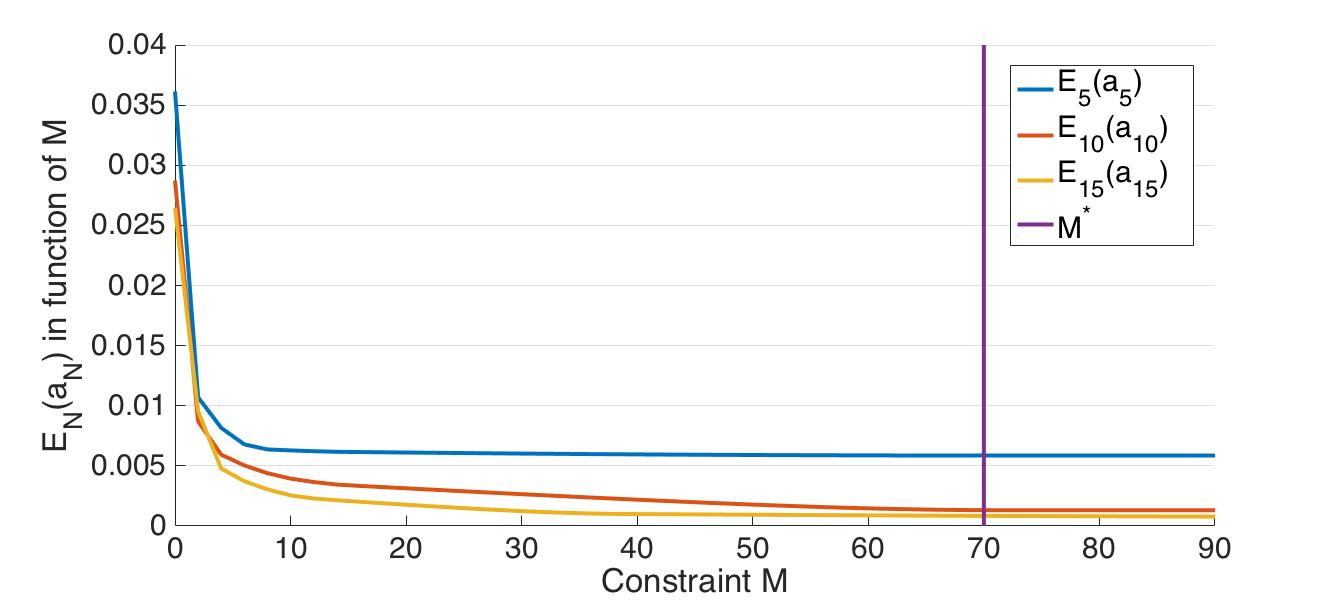
\includegraphics[width=1.2\textwidth]{images/DifferentM3.jpg}
\end{column}
\end{columns}}
}

\frame{
\frametitle{Minimizing $\mathcal E_N$ is a least squares minimization}
\justifying
\vspace{-0.2cm}
The advantage of minimizing $\mathcal E_N(\widehat a)$ is that it can be reduced to a simple {\color{red}$\ell_2$ minimization}. Indeed
\pause
\begin{itemize}
\justifying
\item let $V_N = \operatorname{span}\{\varphi_{\lambda}\}_{\lambda = 1}^{D(N)}$ where the $\varphi_{\lambda}$ are a {\color{blue}linear B-spline basis} with $D(N) $ elements supported on $[0,2R]$,
\pause
\item let $0 = t_0 < t_1 < \ldots < t_m = T$ be a time discretization,
\pause
\item let $\dot{x}_i(t_k) = \frac{x_i(t_k) - x_i(t_{k-1})}{t_k - t_{k-1}}, \text{ for every } k \geq 1$ be the {\color{blue}finite differences} approximating the true velocities,
\end{itemize}
\pause
then the {\color{red}\textit{discrete-time error functional}} satisfies
\footnotesize{
\begin{align*}
\overline{\mathcal{E}}_N(\widehat{a}) & = \frac{1}{m} \sum^m_{k = 1} \frac{1}{N} \sum^N_{j = 1} \left| \sum^{D(N)}_{\lambda = 1}\frac{a_{\lambda}}{N} \sum^N_{i = 1} \varphi_{\lambda}(|x_j(t_k) - x_i(t_k)|)(x_j(t_k) - x_i(t_k)) - \dot{x}_i(t_k)\right|^2\\
\pause
& = {\color{blue}\frac{1}{mN} \left\| C \vec{a} - v \right\|^2_{2}}.
\end{align*}}
\pause
where $\vec{a} = (a_1, \ldots, a_{D(N)})$, $v = (\dot{x}_1(t_1), \ldots, \dot{x}_N(t_1), \ldots,\dot{x}_1(t_m), \ldots, \dot{x}_N(t_m))$.
}

\frame{
\frametitle{How we implement the constraints}
\justifying
If $D = \begin{bmatrix}
    1       & -1 & \dots & 0 & 0 \\
   \vdots & \vdots & \ddots & \ddots & \vdots \\ \\
    0       & 0 & \dots & 1 & -1 \\
    0       & 0 & \dots & 0 & 0
\end{bmatrix}$then
\begin{align*}
\|a\|_{L_{\infty}([0,2R])} \leq 2 \|\vec{a}\|_{\infty} &\text{ and } \|a'\|_{L_{\infty}([0,2R])} \leq \|D\vec{a}\|_{\infty},
\end{align*}
\pause
hence we numerically implement the convex constrained minimization
\begin{align*}
\min_{\widehat{a} \in V_N} \mathcal{E}_N(\widehat{a}) \quad \text{ subject to } \quad \|\widehat{a}\|_{L_{\infty}([0,R])} + \|\widehat{a}'\|_{L_{\infty}([0,R])} \leq M,
\end{align*}
in the following way
{\color{blue}\begin{align*}
\min_{\vec{a} \in \R^{D(N)}} \frac{1}{mN} \left\| C \vec{a} - v \right\|^2_{2} \quad \text{ subject to } \quad 2\|\vec{a}\|_{\infty} + \|D\vec{a}\|_{\infty} \leq M.
\end{align*}}
}

\frame{
\frametitle{Varying $N$ - I}
\justifying
\vspace{-0.2cm}
\begin{table}[h]
\begin{center}
\begin{tabular}{ |c|c|c|c|c|c| }
\hline
  $d$ & $L$ & $T$ & $M$ & $N$ & $D(N)$ \\
\hline
\hline
  $2$ & $3$ & $0.5$ & $100$ & $[10,20,40,80]$ & $2N$ \\
\hline
\end{tabular}
\end{center}
\vspace{-0.1cm}
\caption{Parameter values}
\end{table}
\vspace{-0.2cm}
\begin{figure}[h!]
\begin{center}
\visible<1->{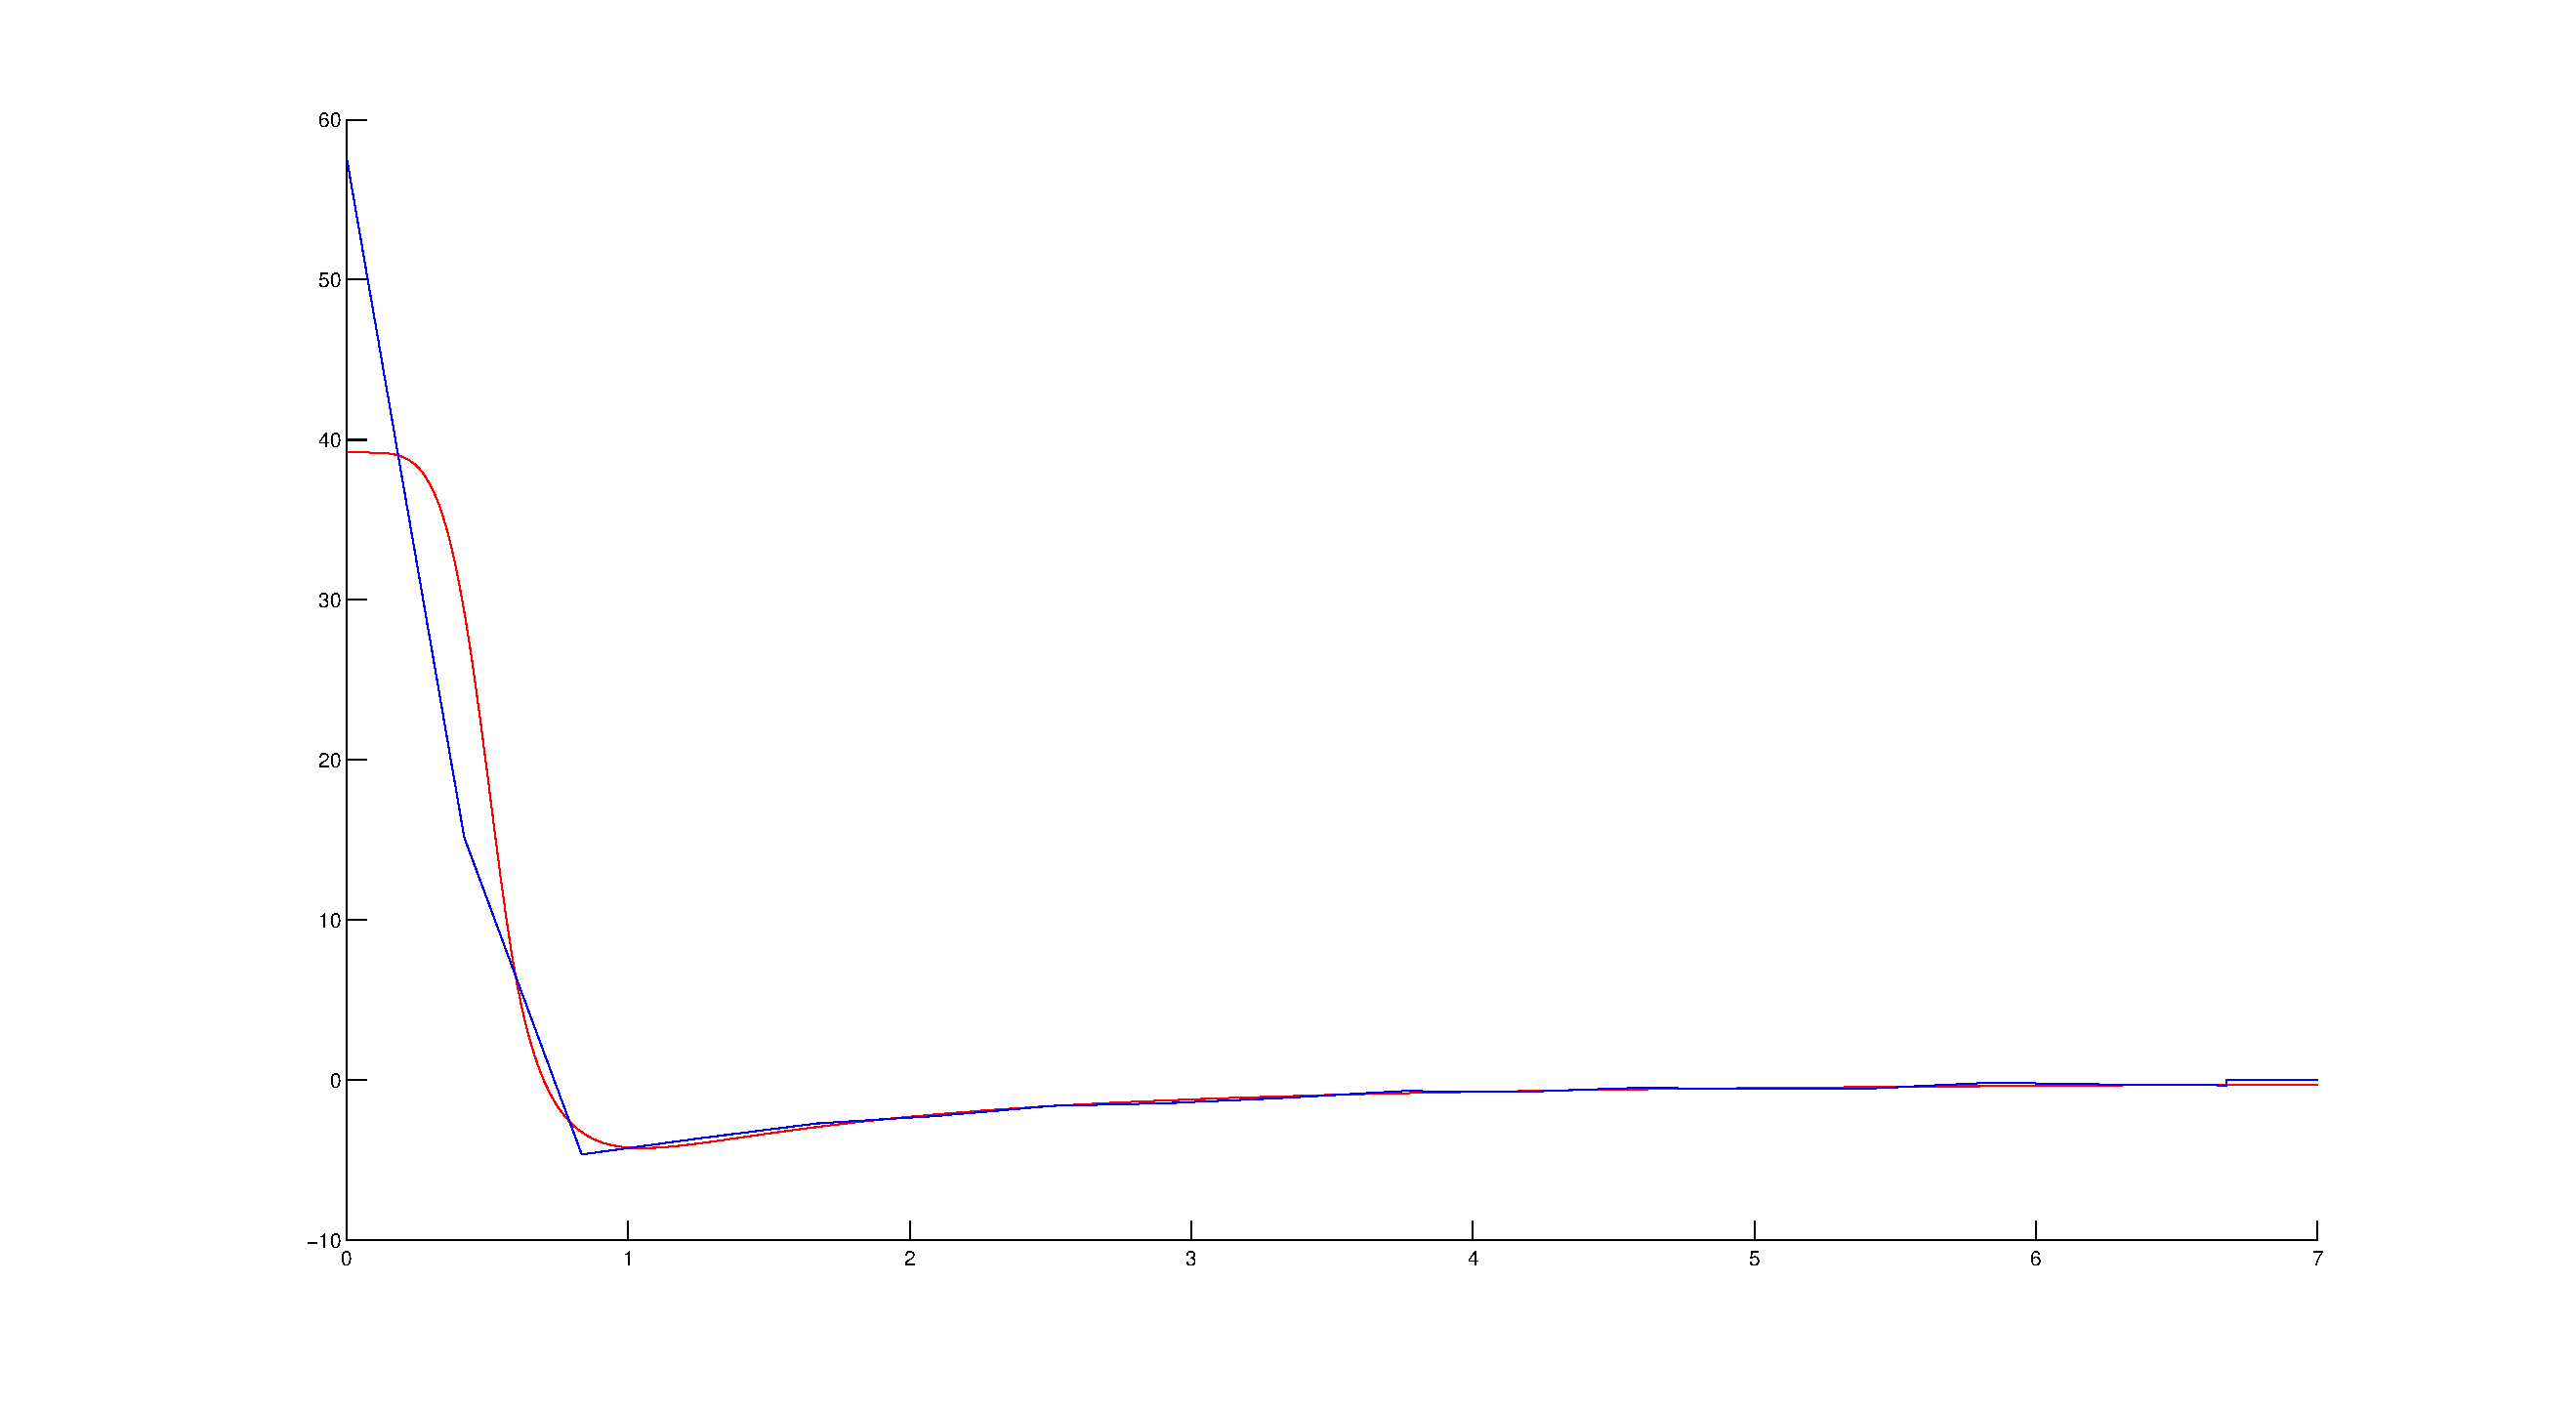
\includegraphics[width=0.45\textwidth]{Figures/figfun810agents}}\pause
\visible<2->{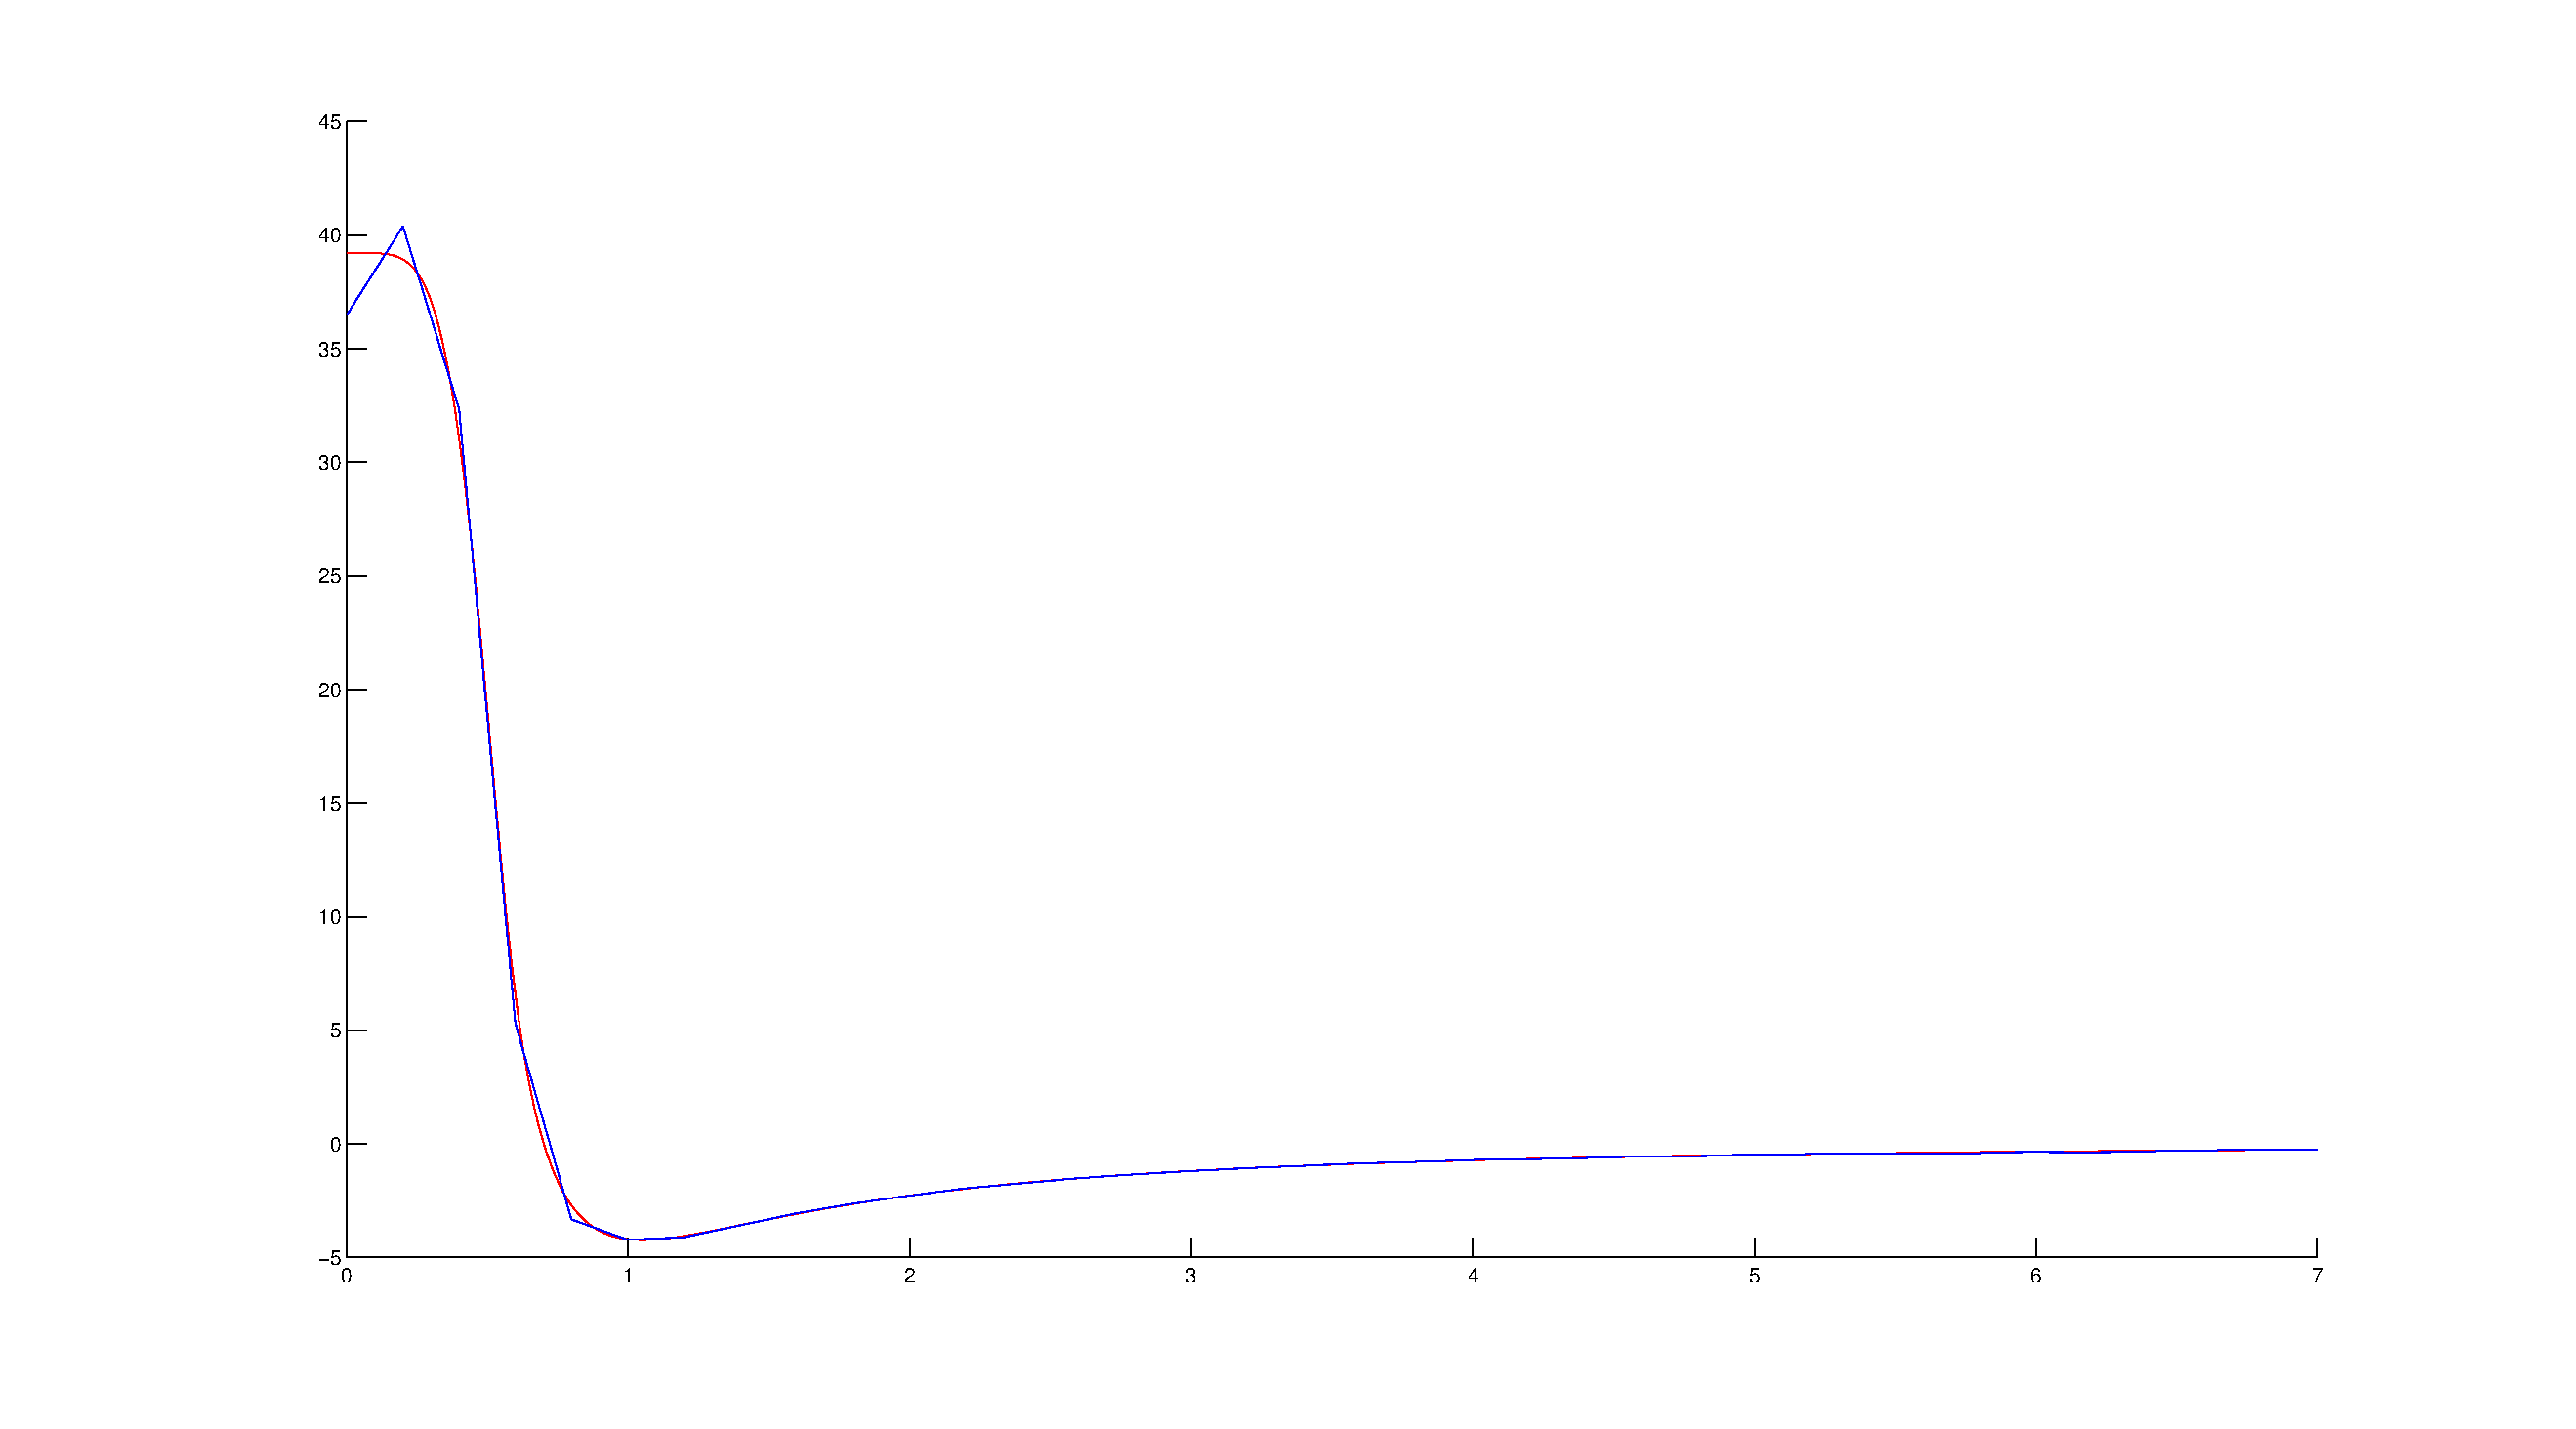
\includegraphics[width=0.45\textwidth]{Figures/figfun820agents}}\pause\\
\visible<3->{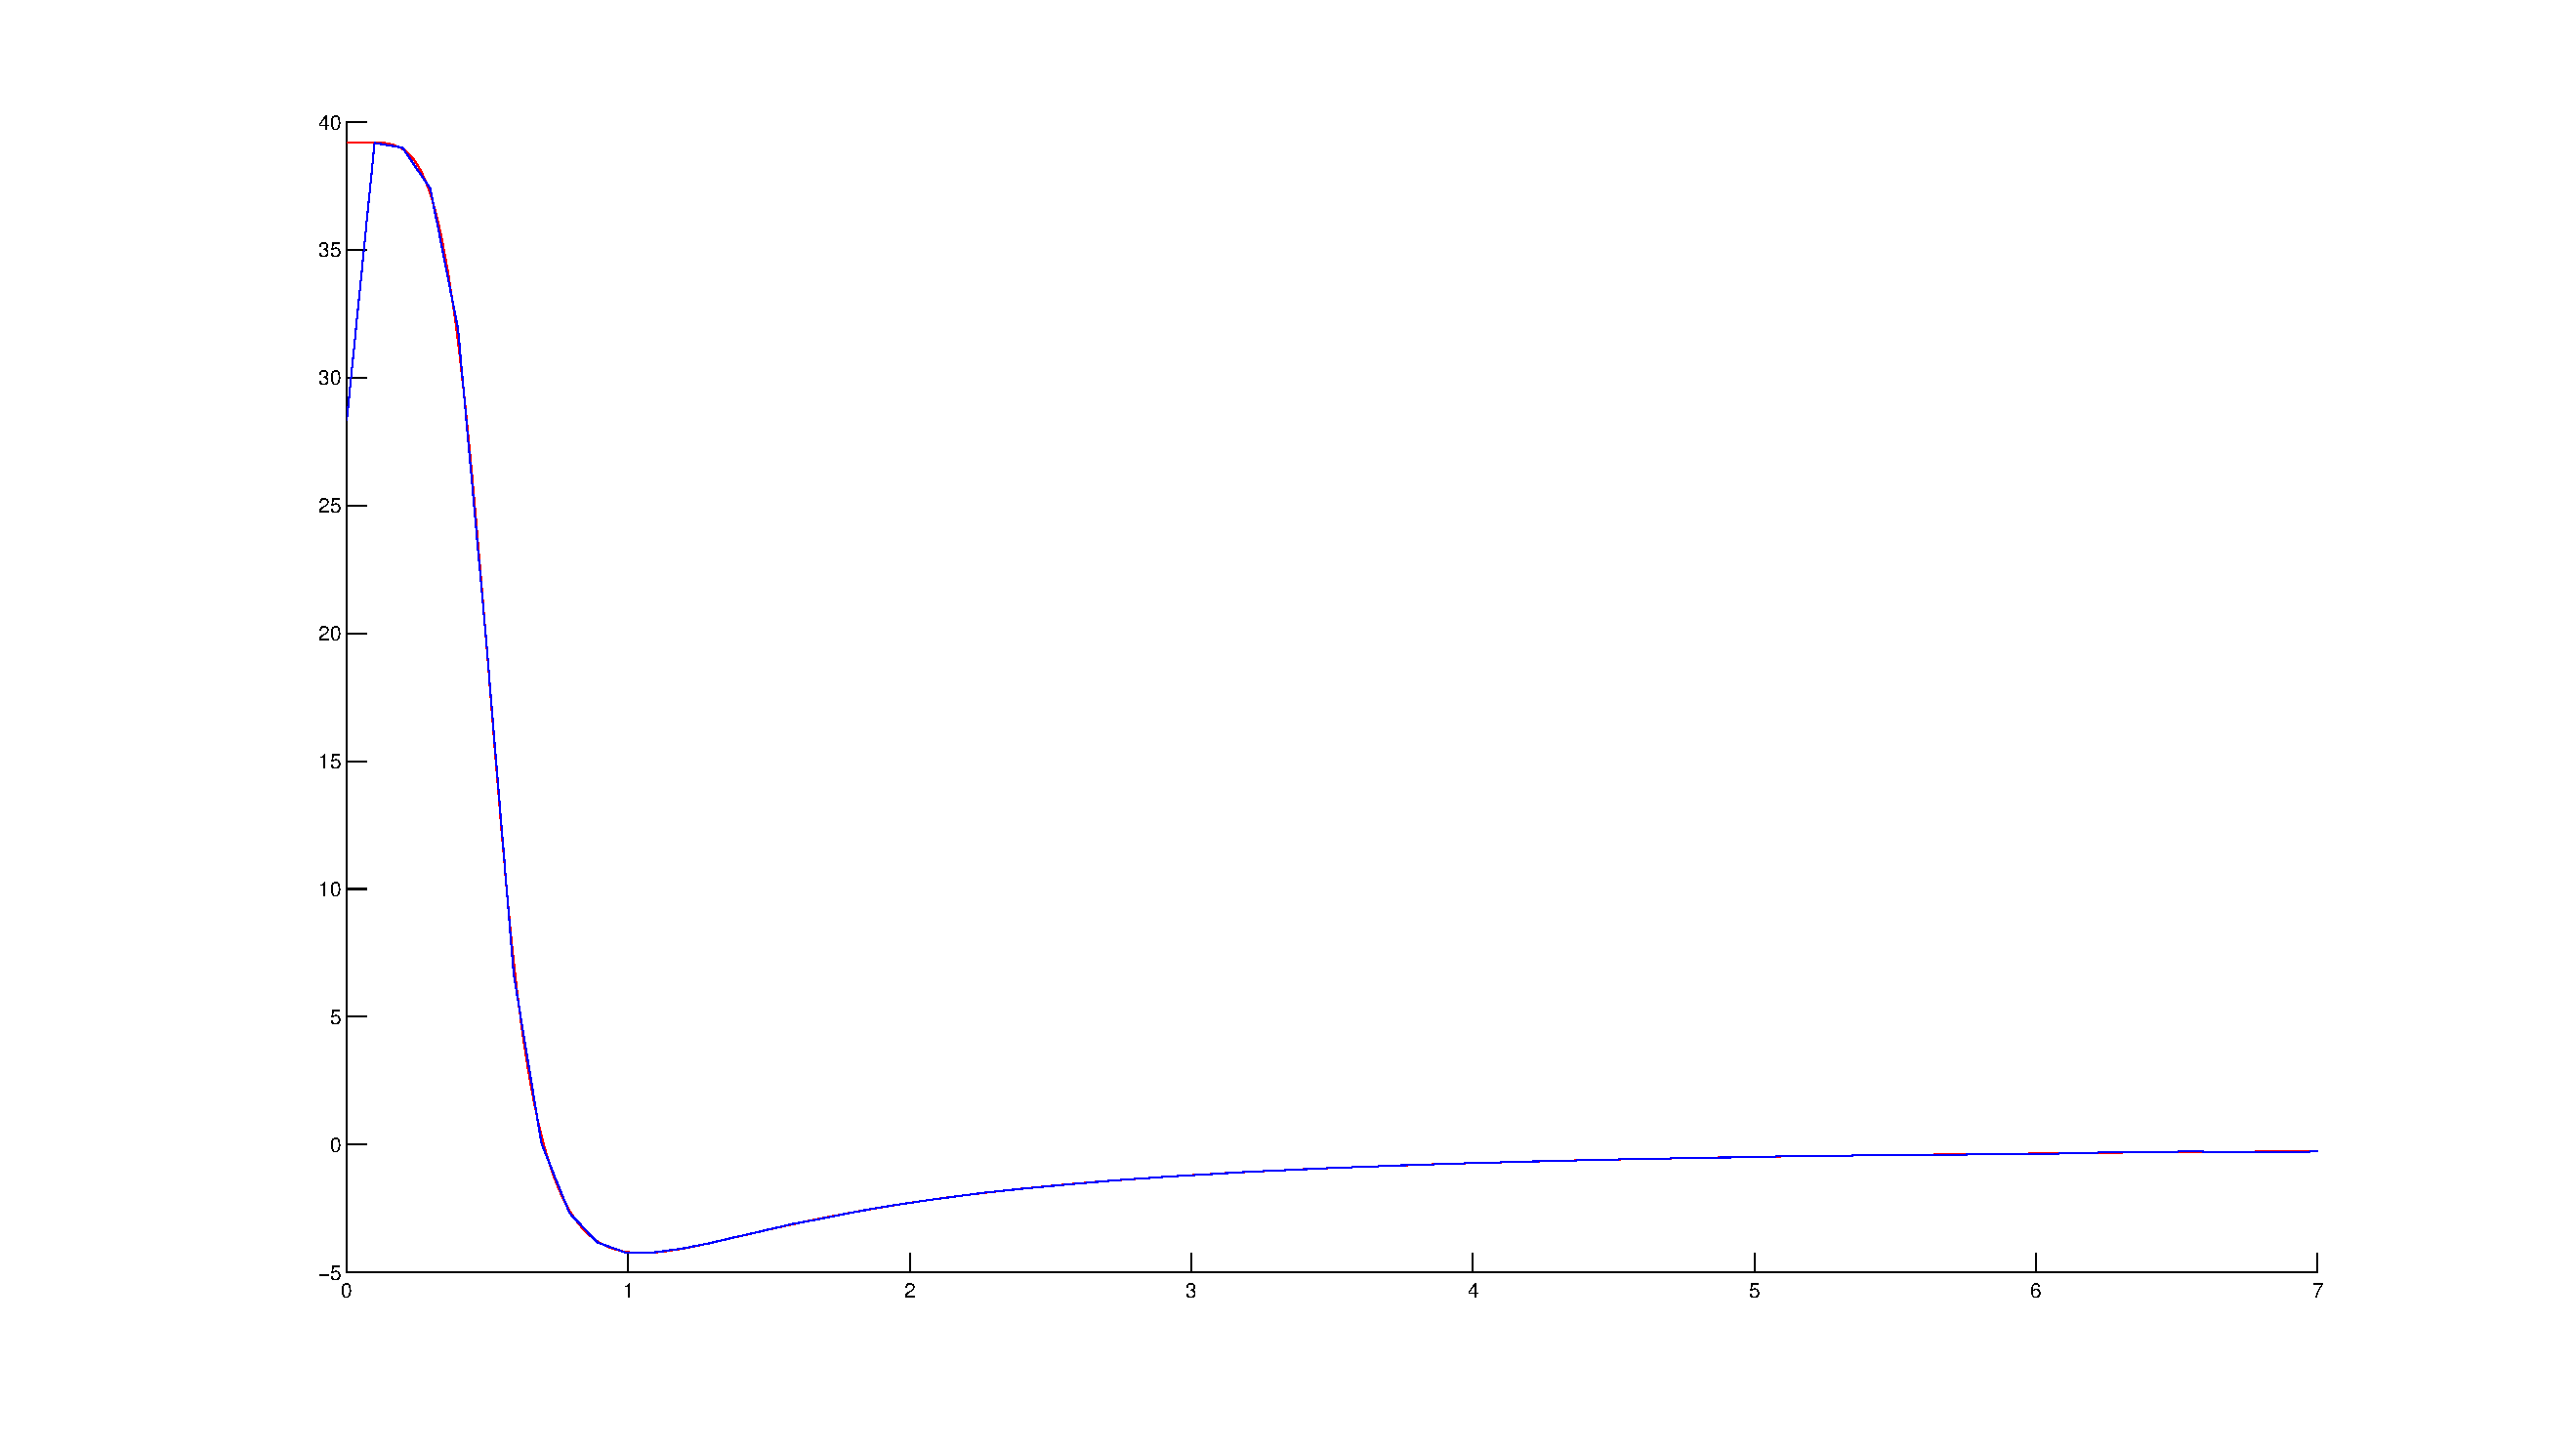
\includegraphics[width=0.45\textwidth]{Figures/figfun840agents}}\pause
\visible<4->{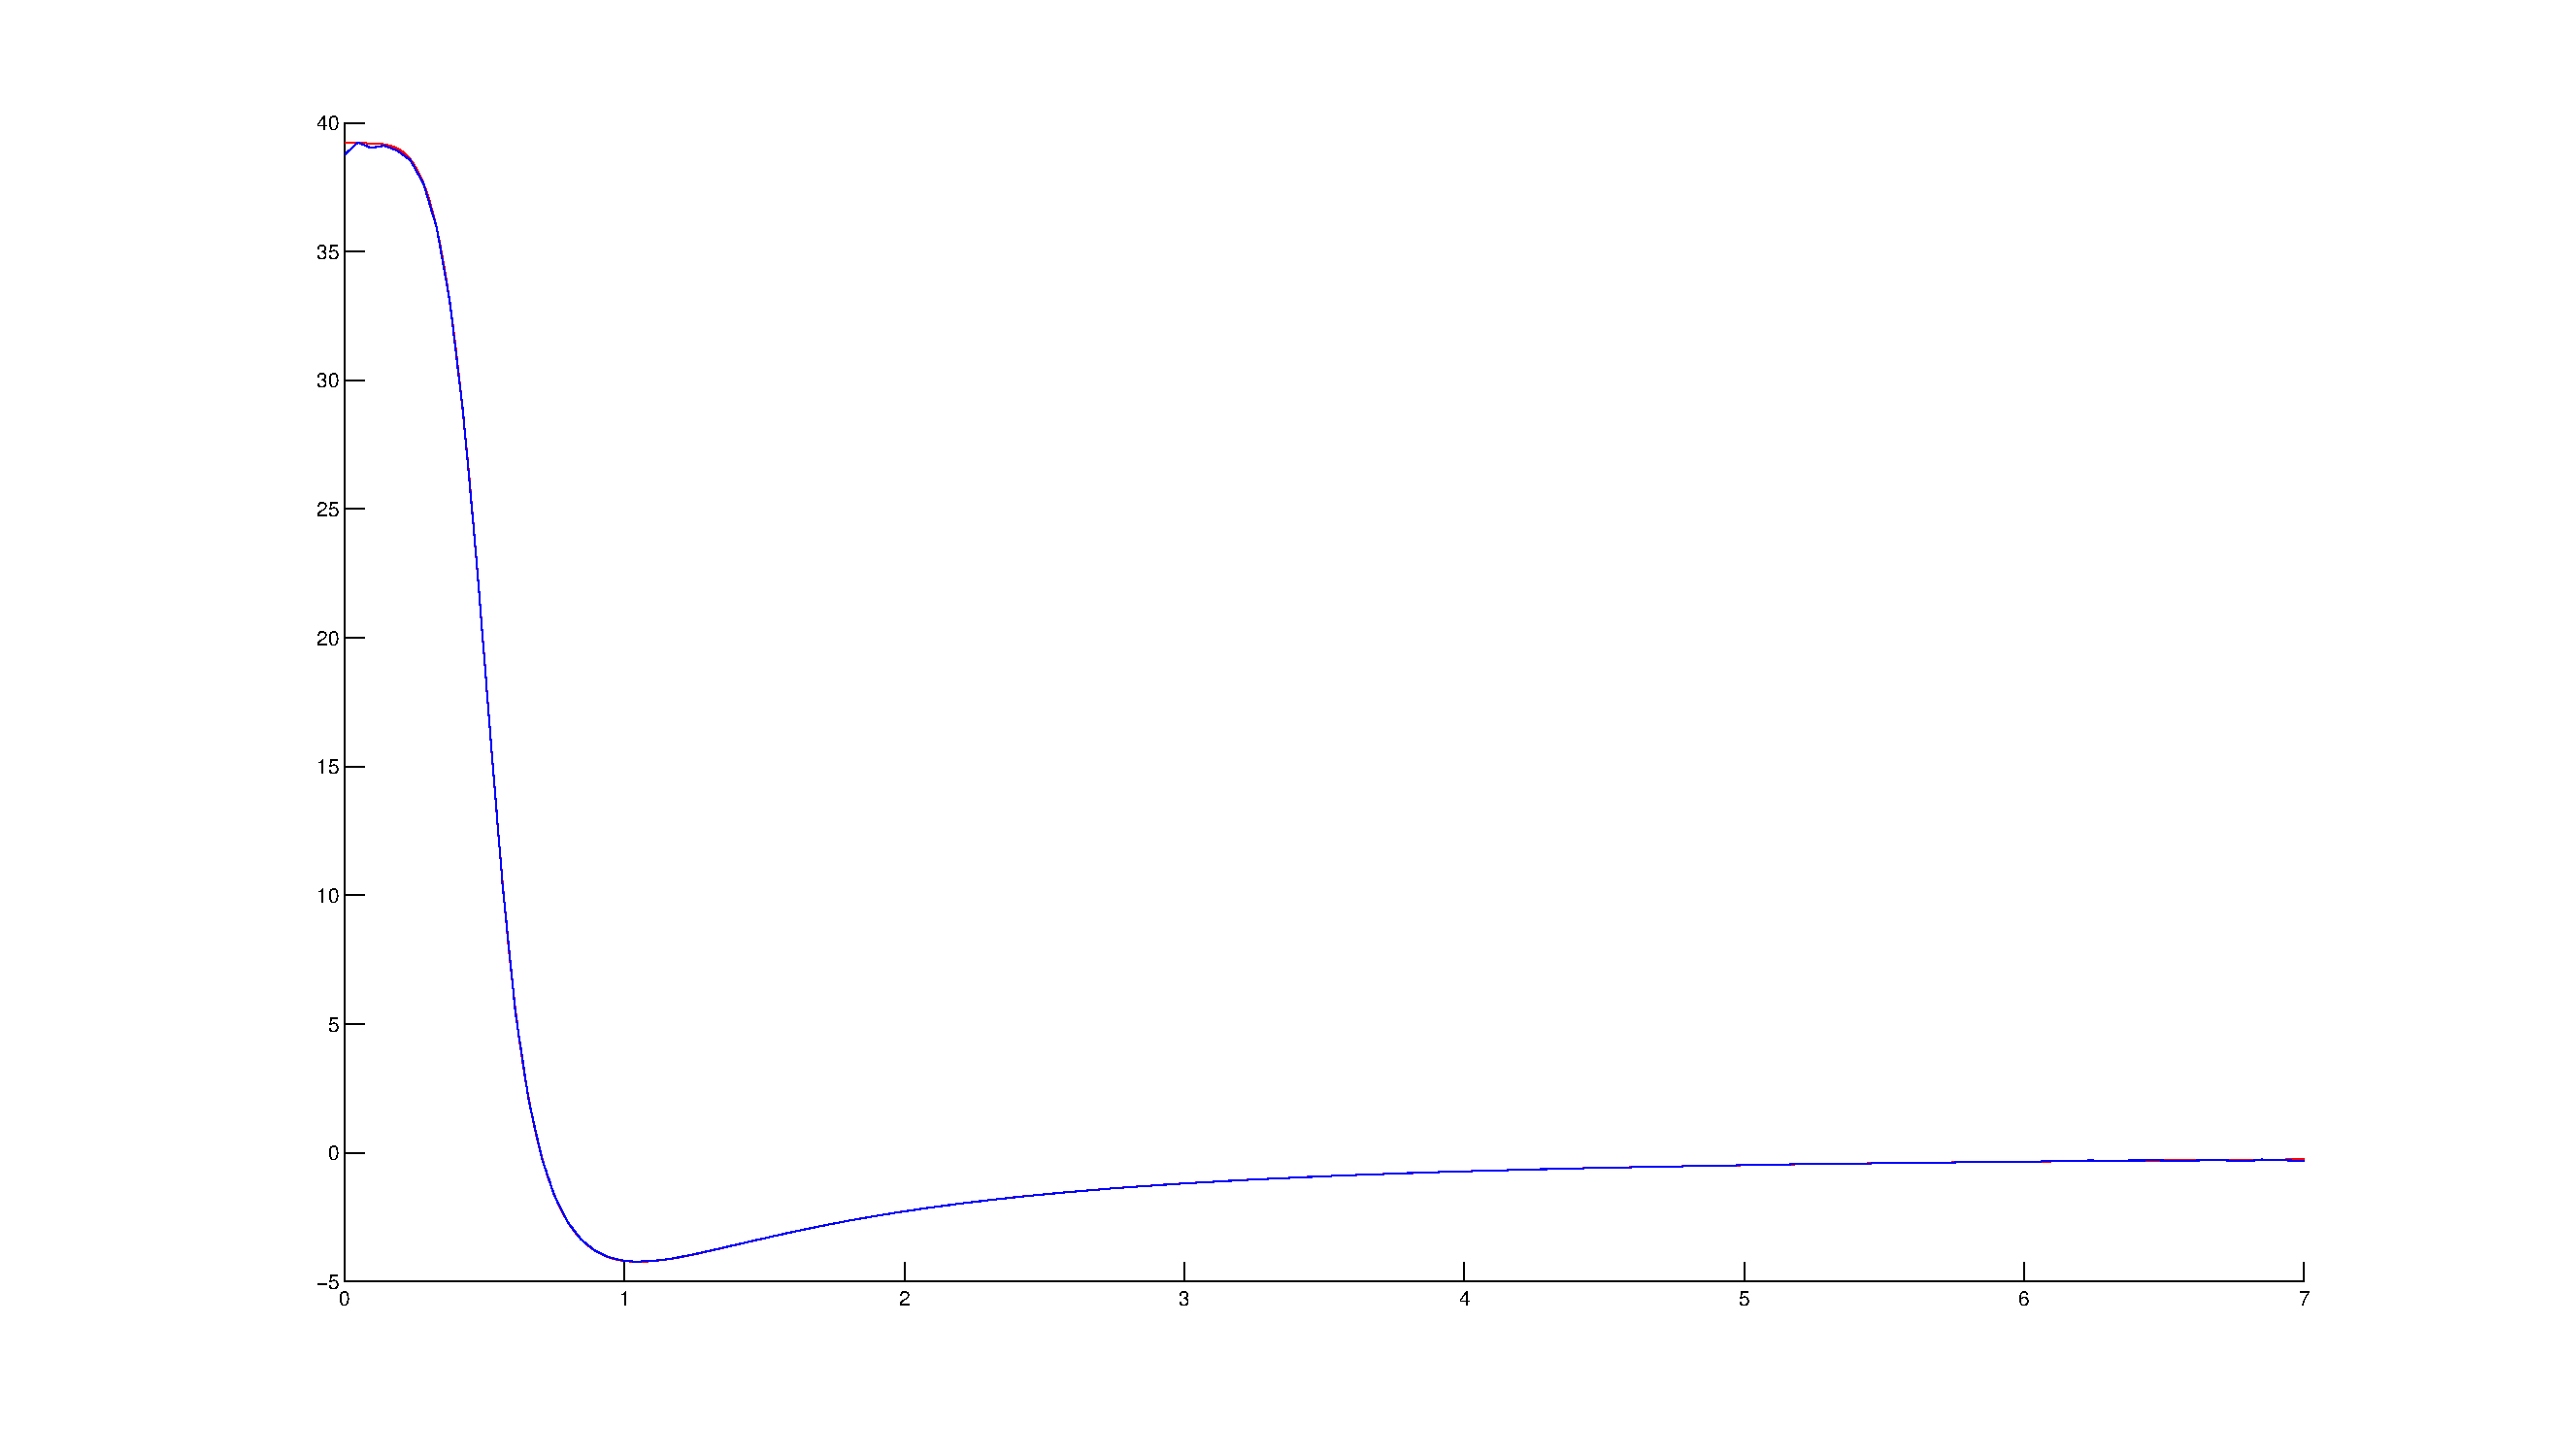
\includegraphics[width=0.45\textwidth]{Figures/figfun880agents}}
\end{center}
\end{figure}
}

\frame{
\frametitle{Varying $N$ - II}
\justifying
\vspace{-0.1cm}
\begin{table}[h]
\begin{center}
\begin{tabular}{ |c|c|c|c|c|c| }
\hline
  $d$ & $L$ & $T$ & $M$ & $N$ & $D(N)$ \\
\hline
\hline
  $2$ & $3$ & $0.5$ & $100$ & $[10,20,40,80]$ & $2N$ \\
\hline
\end{tabular}
\end{center}
\caption{Parameter values}
\end{table}
\vspace{-0.2cm}
\begin{figure}[h!]
\begin{center}
\visible<1->{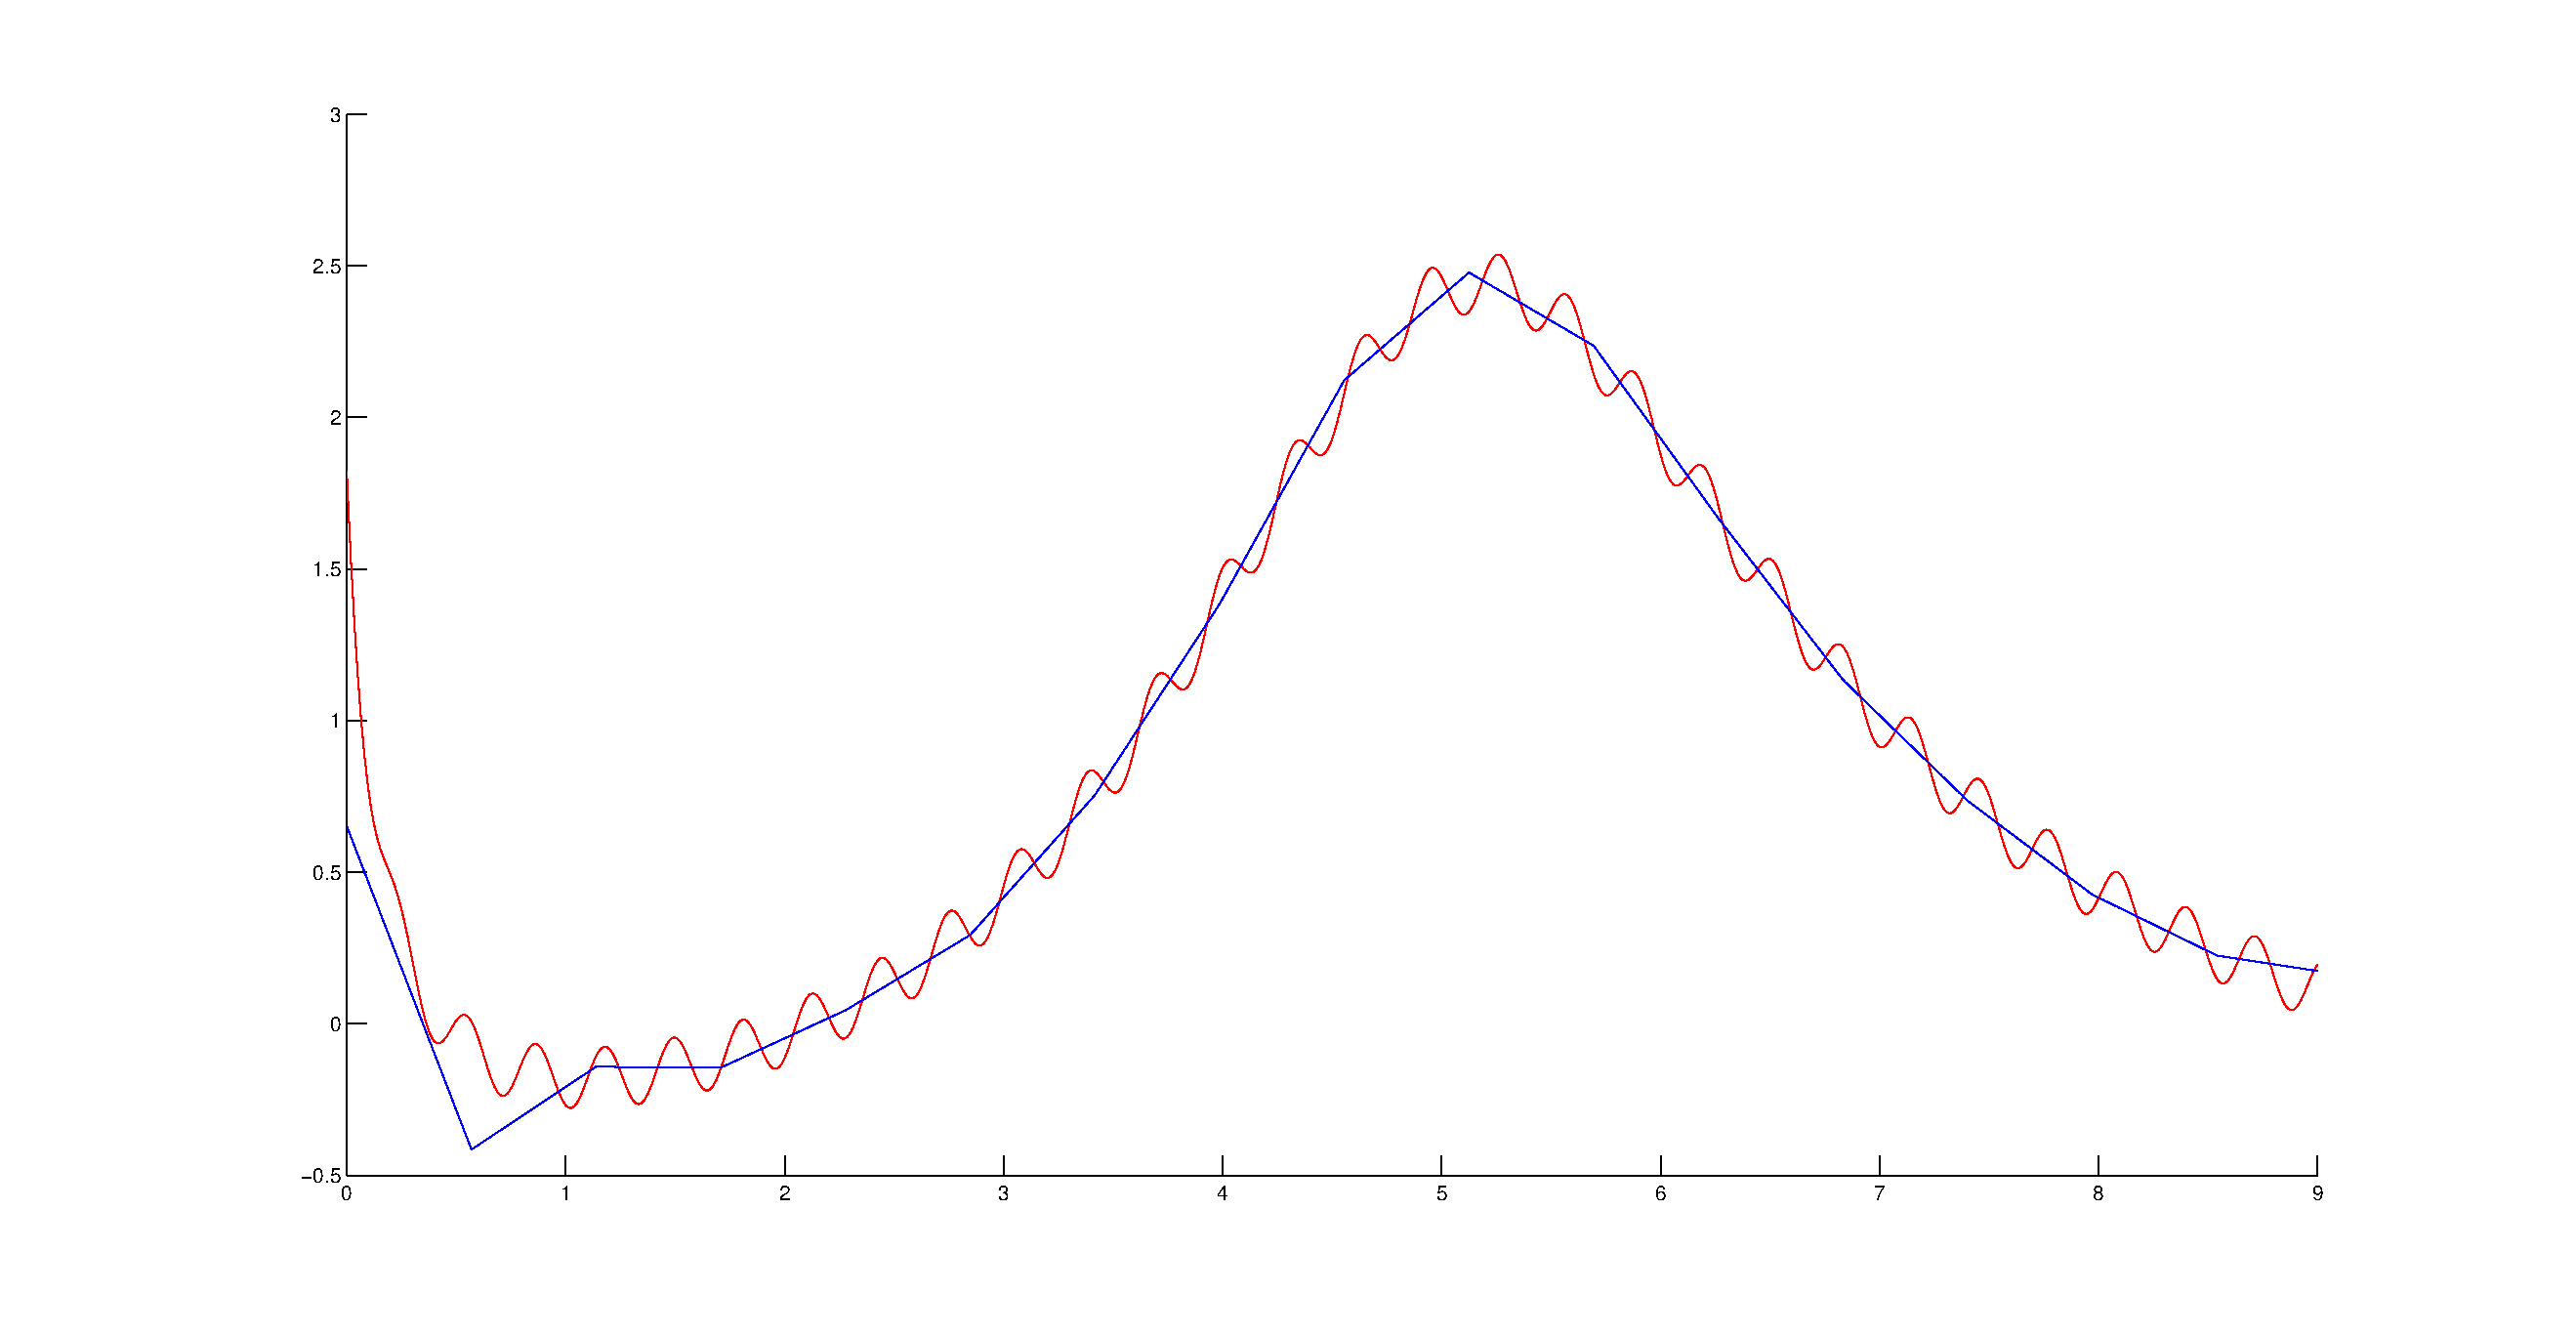
\includegraphics[width=0.45\textwidth]{Figures/figfun610agents}}\pause
\visible<2->{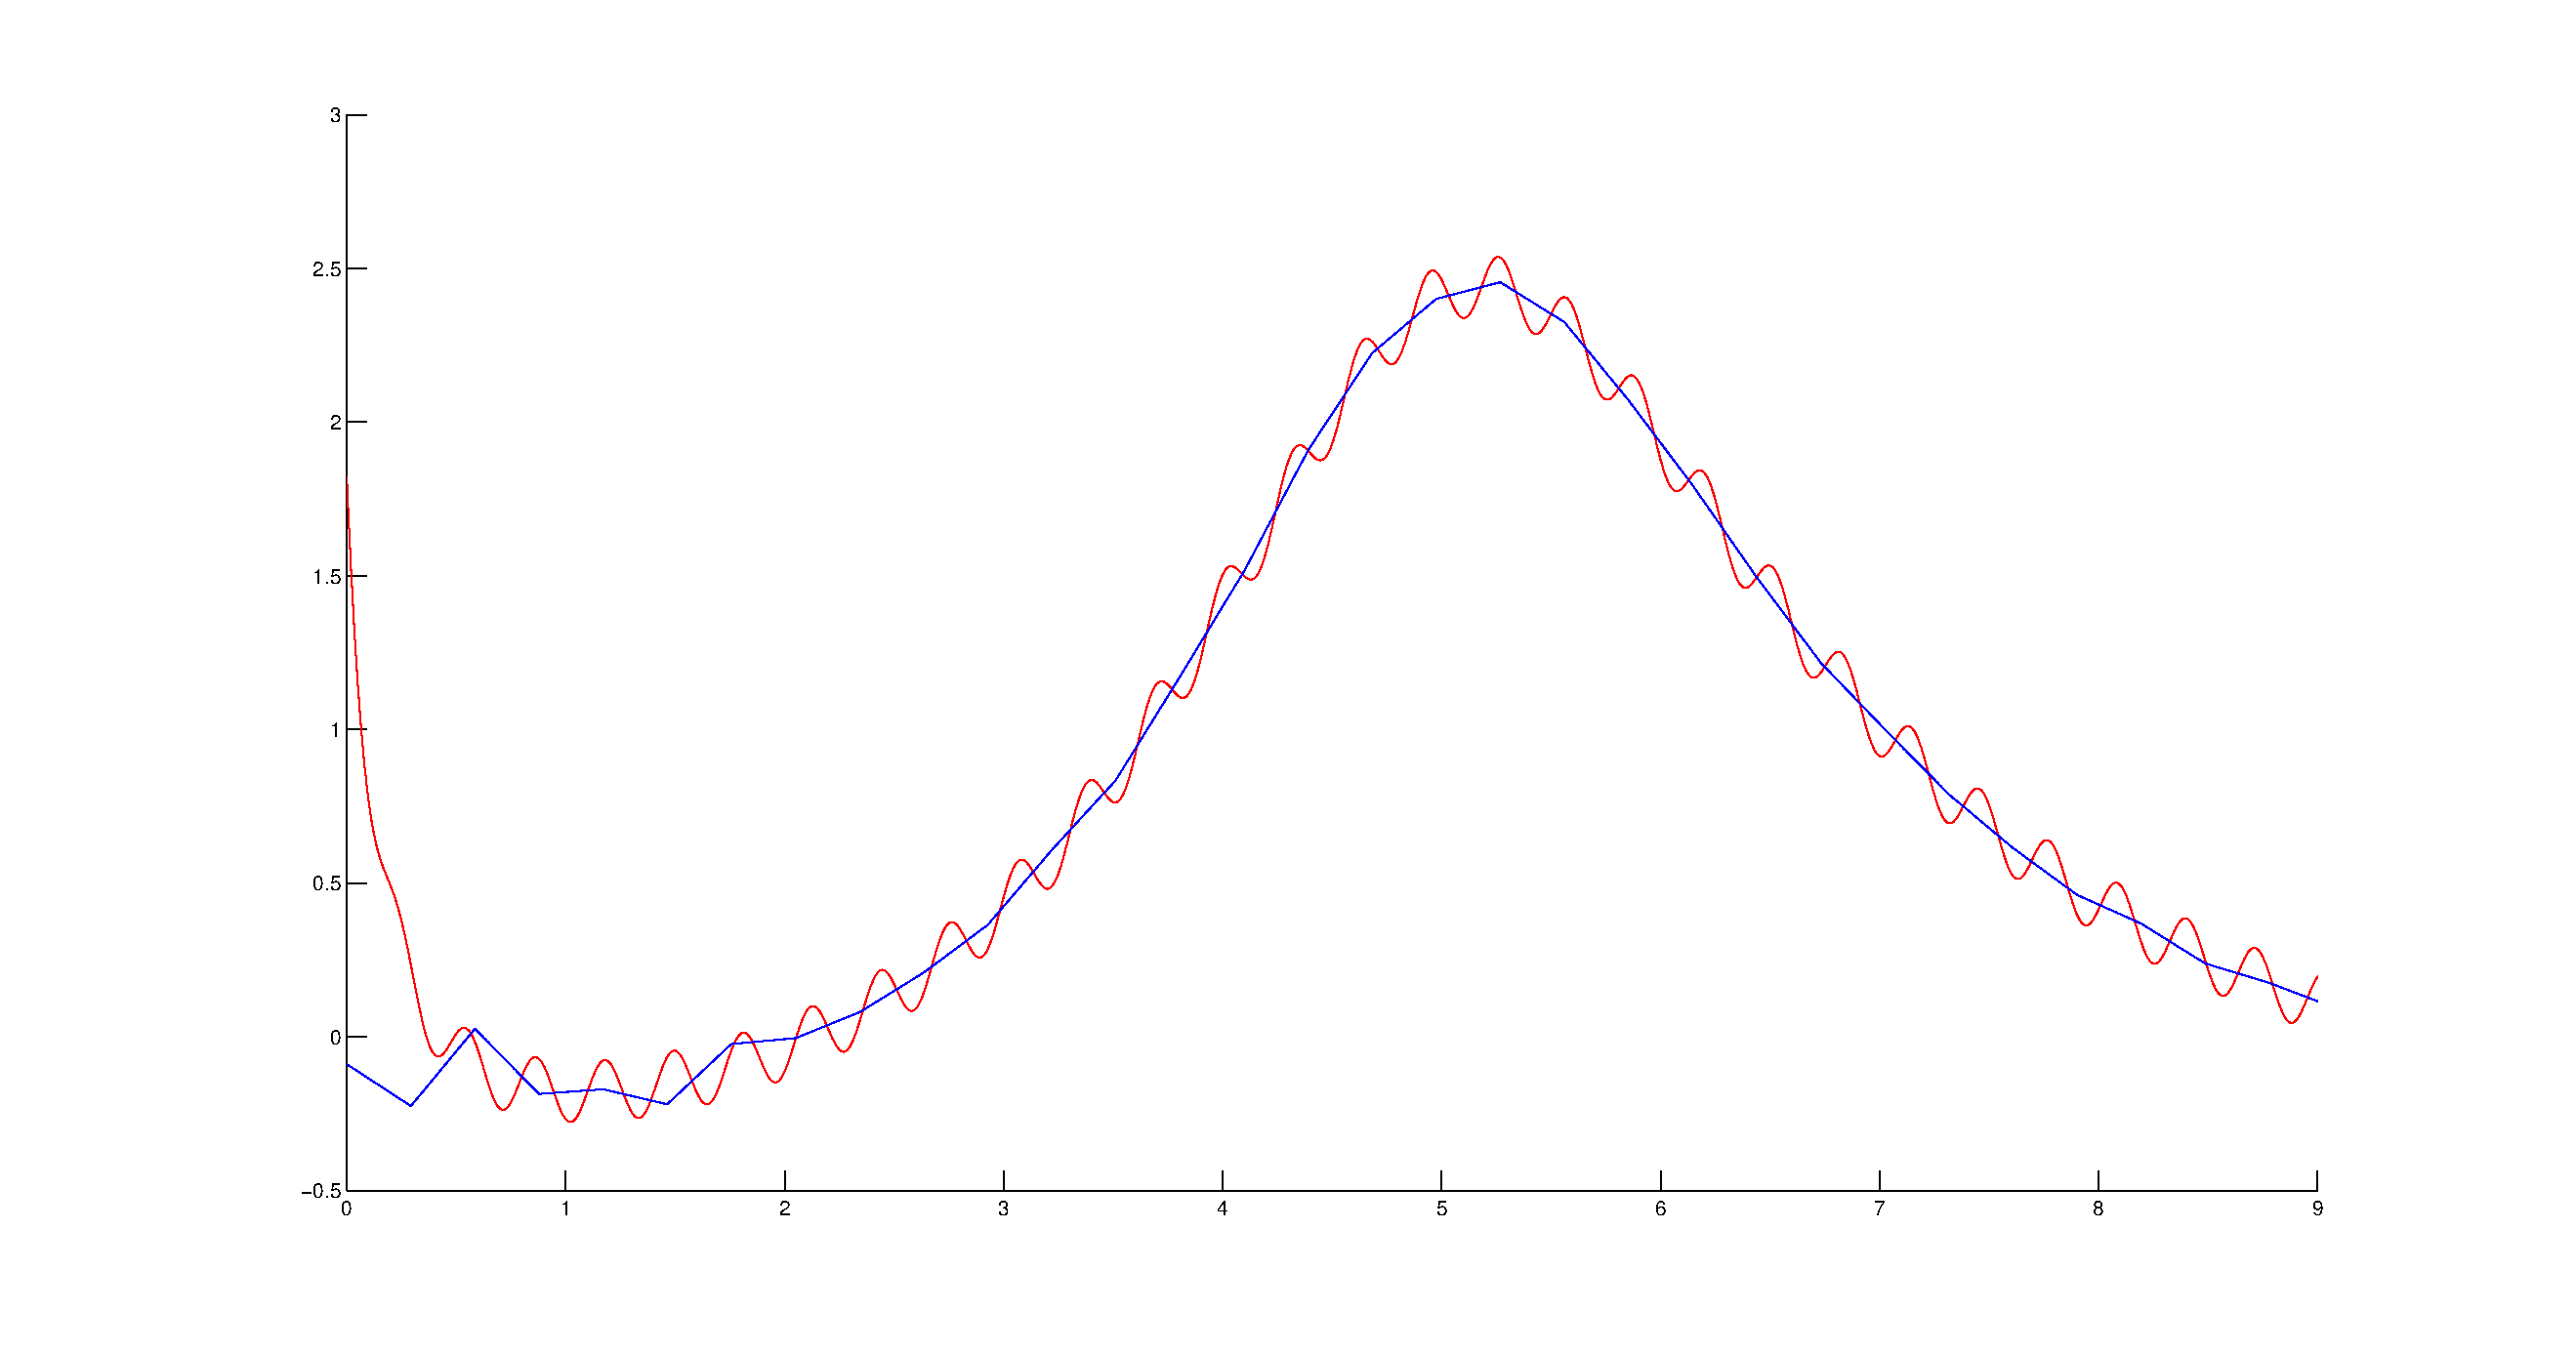
\includegraphics[width=0.45\textwidth]{Figures/figfun620agents}}\pause\\
\visible<3->{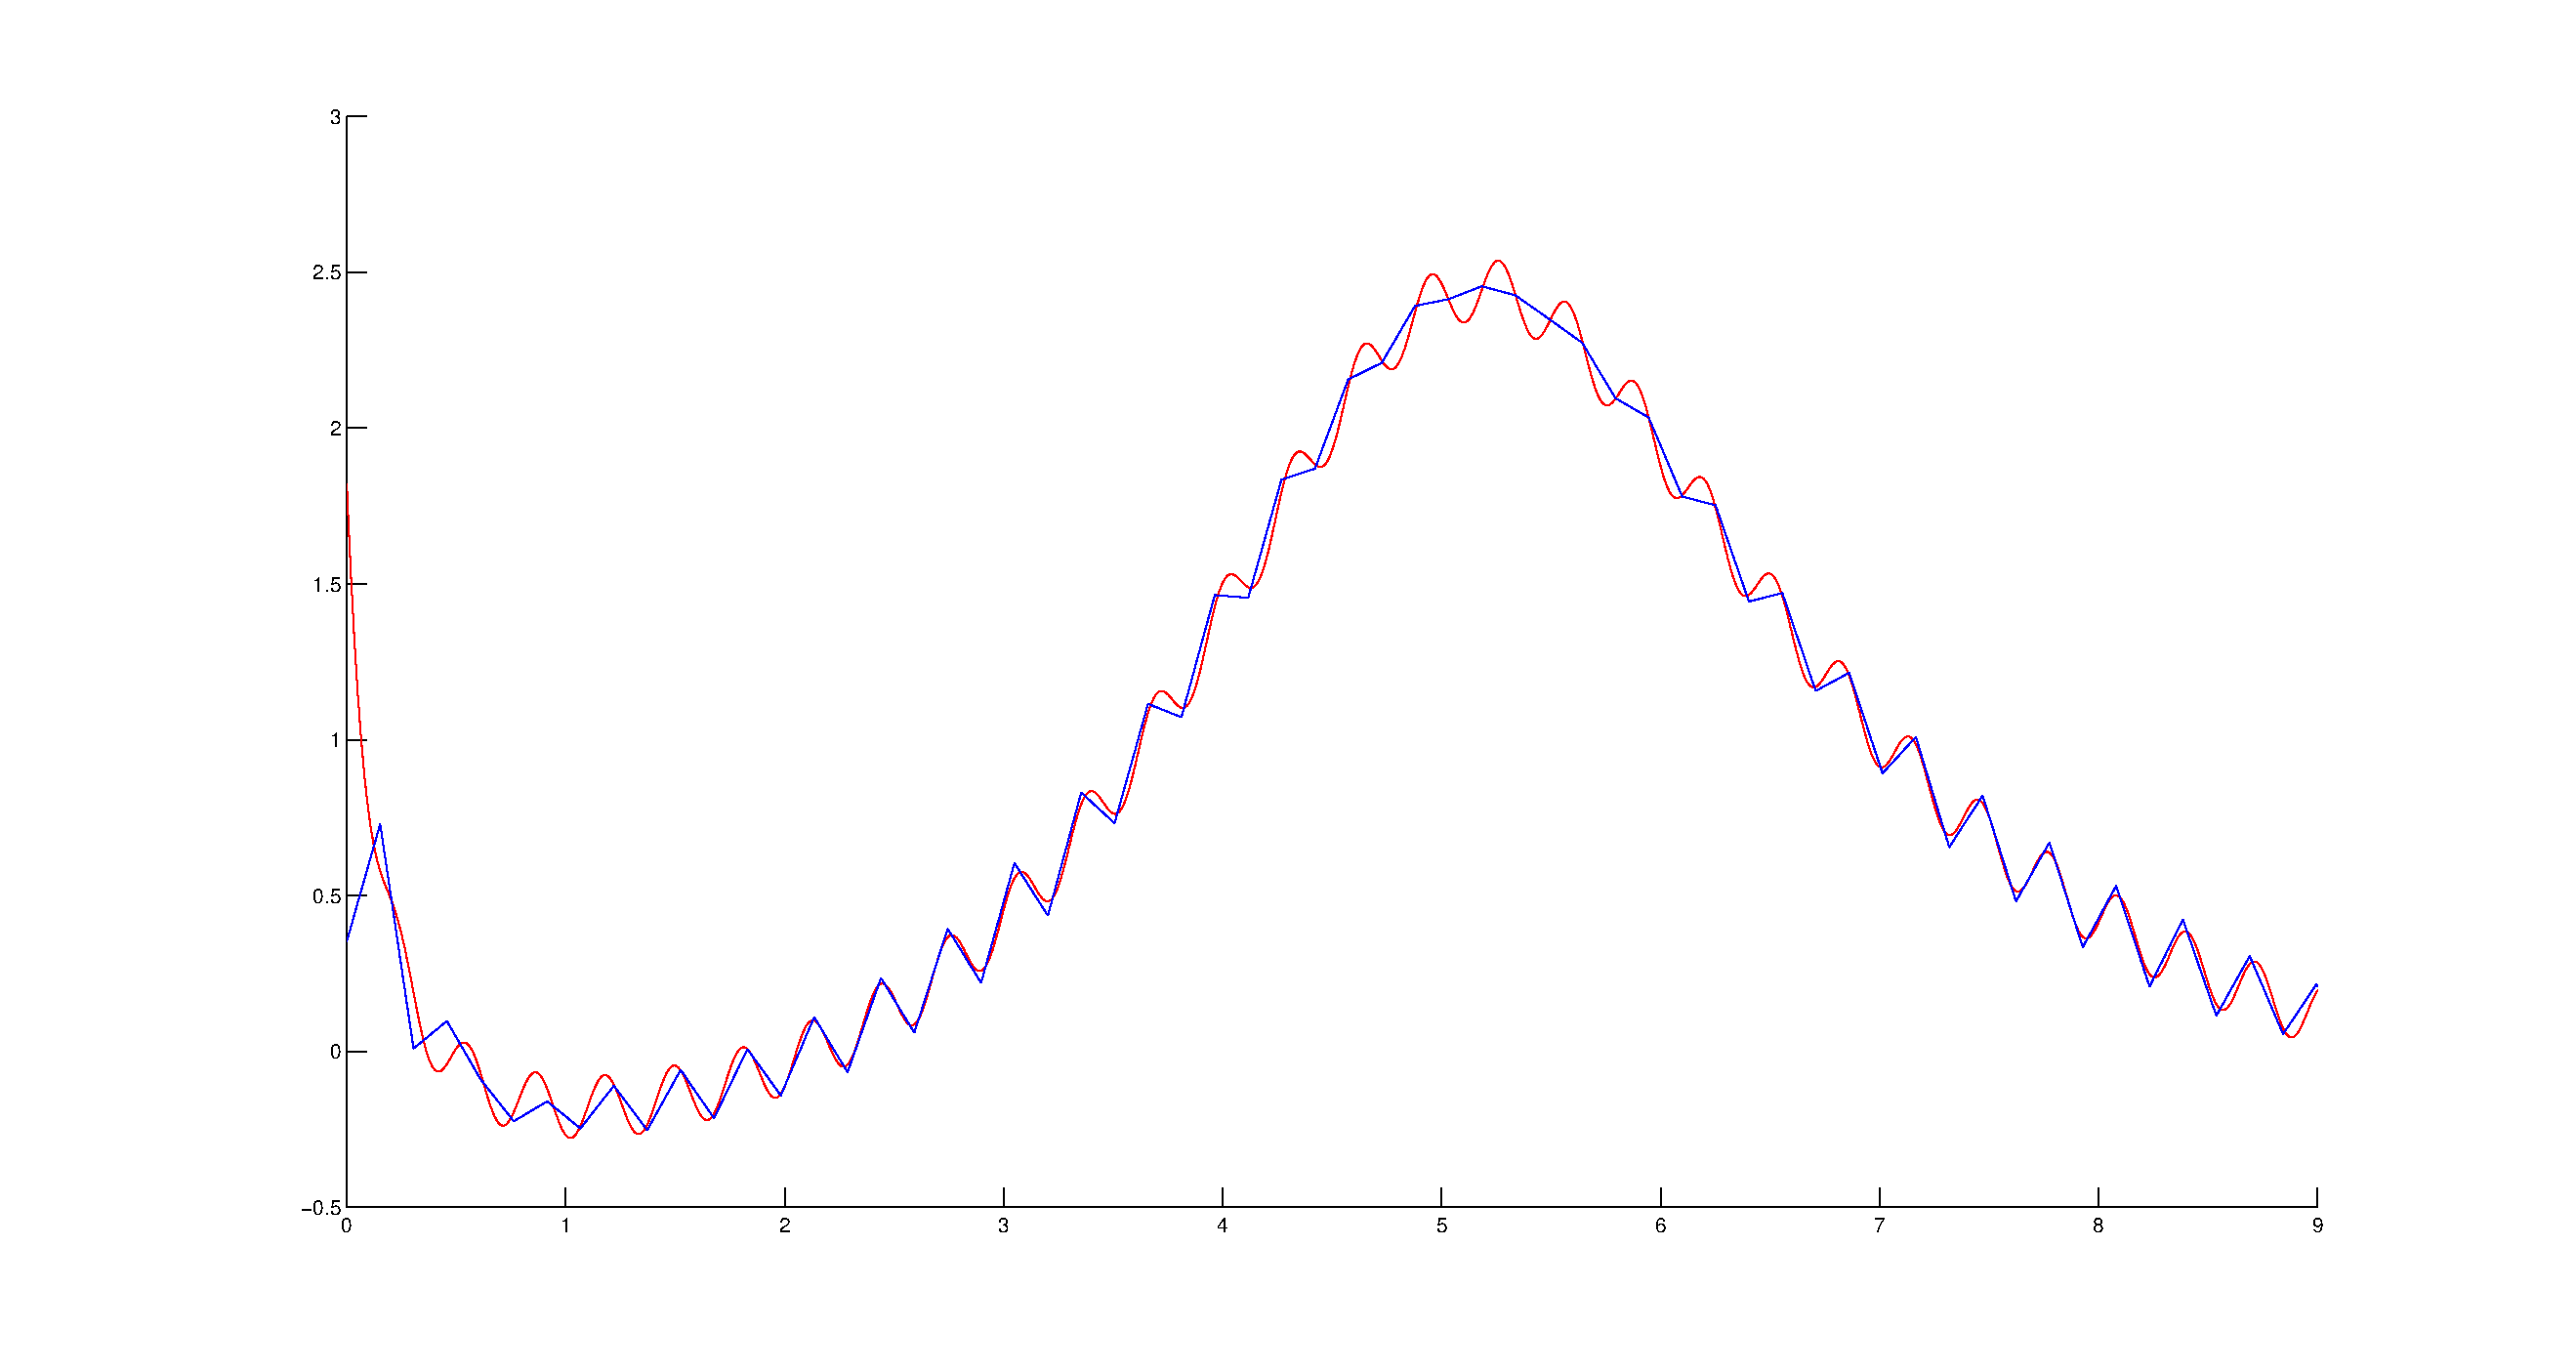
\includegraphics[width=0.45\textwidth]{Figures/figfun640agents}}\pause
\visible<4->{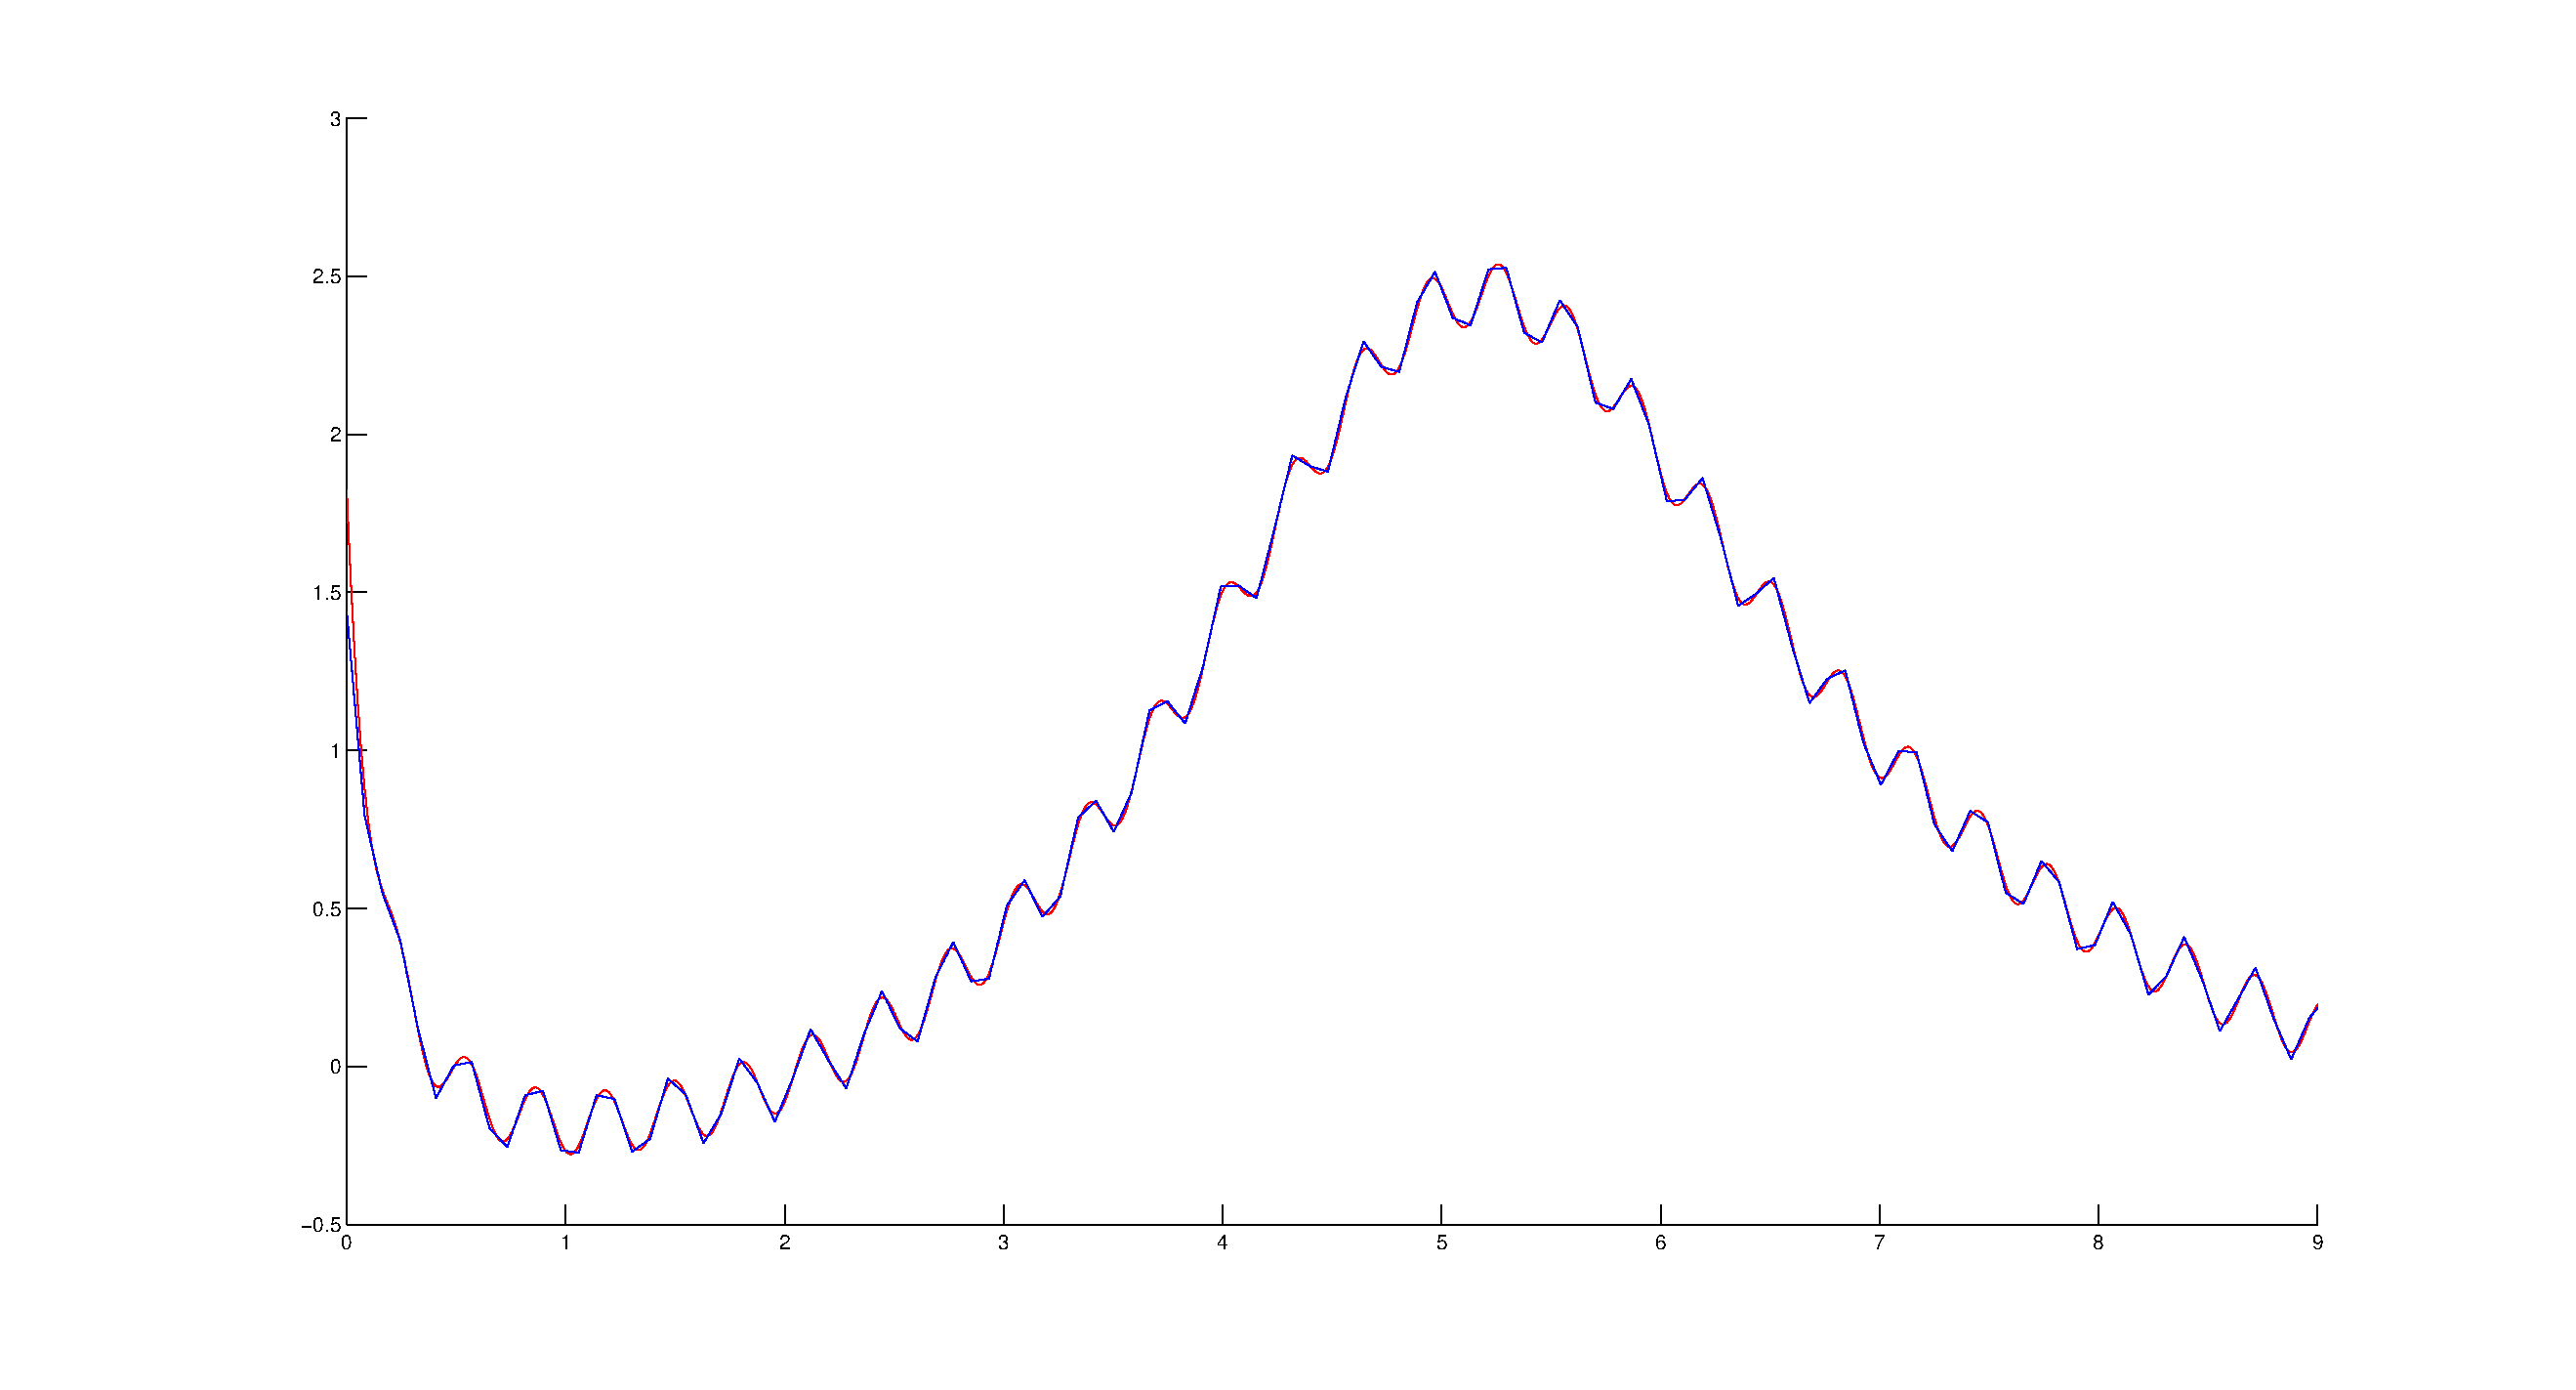
\includegraphics[width=0.45\textwidth]{Figures/figfun680agents}}
\end{center}
\end{figure}
}

%\frame{
%\frametitle{The coercivity constraint}
%\justifying
%\begin{figure}[h]
%\hspace{-0.5cm}
%\begin{minipage}{0.49\textwidth}
%\begin{center}
%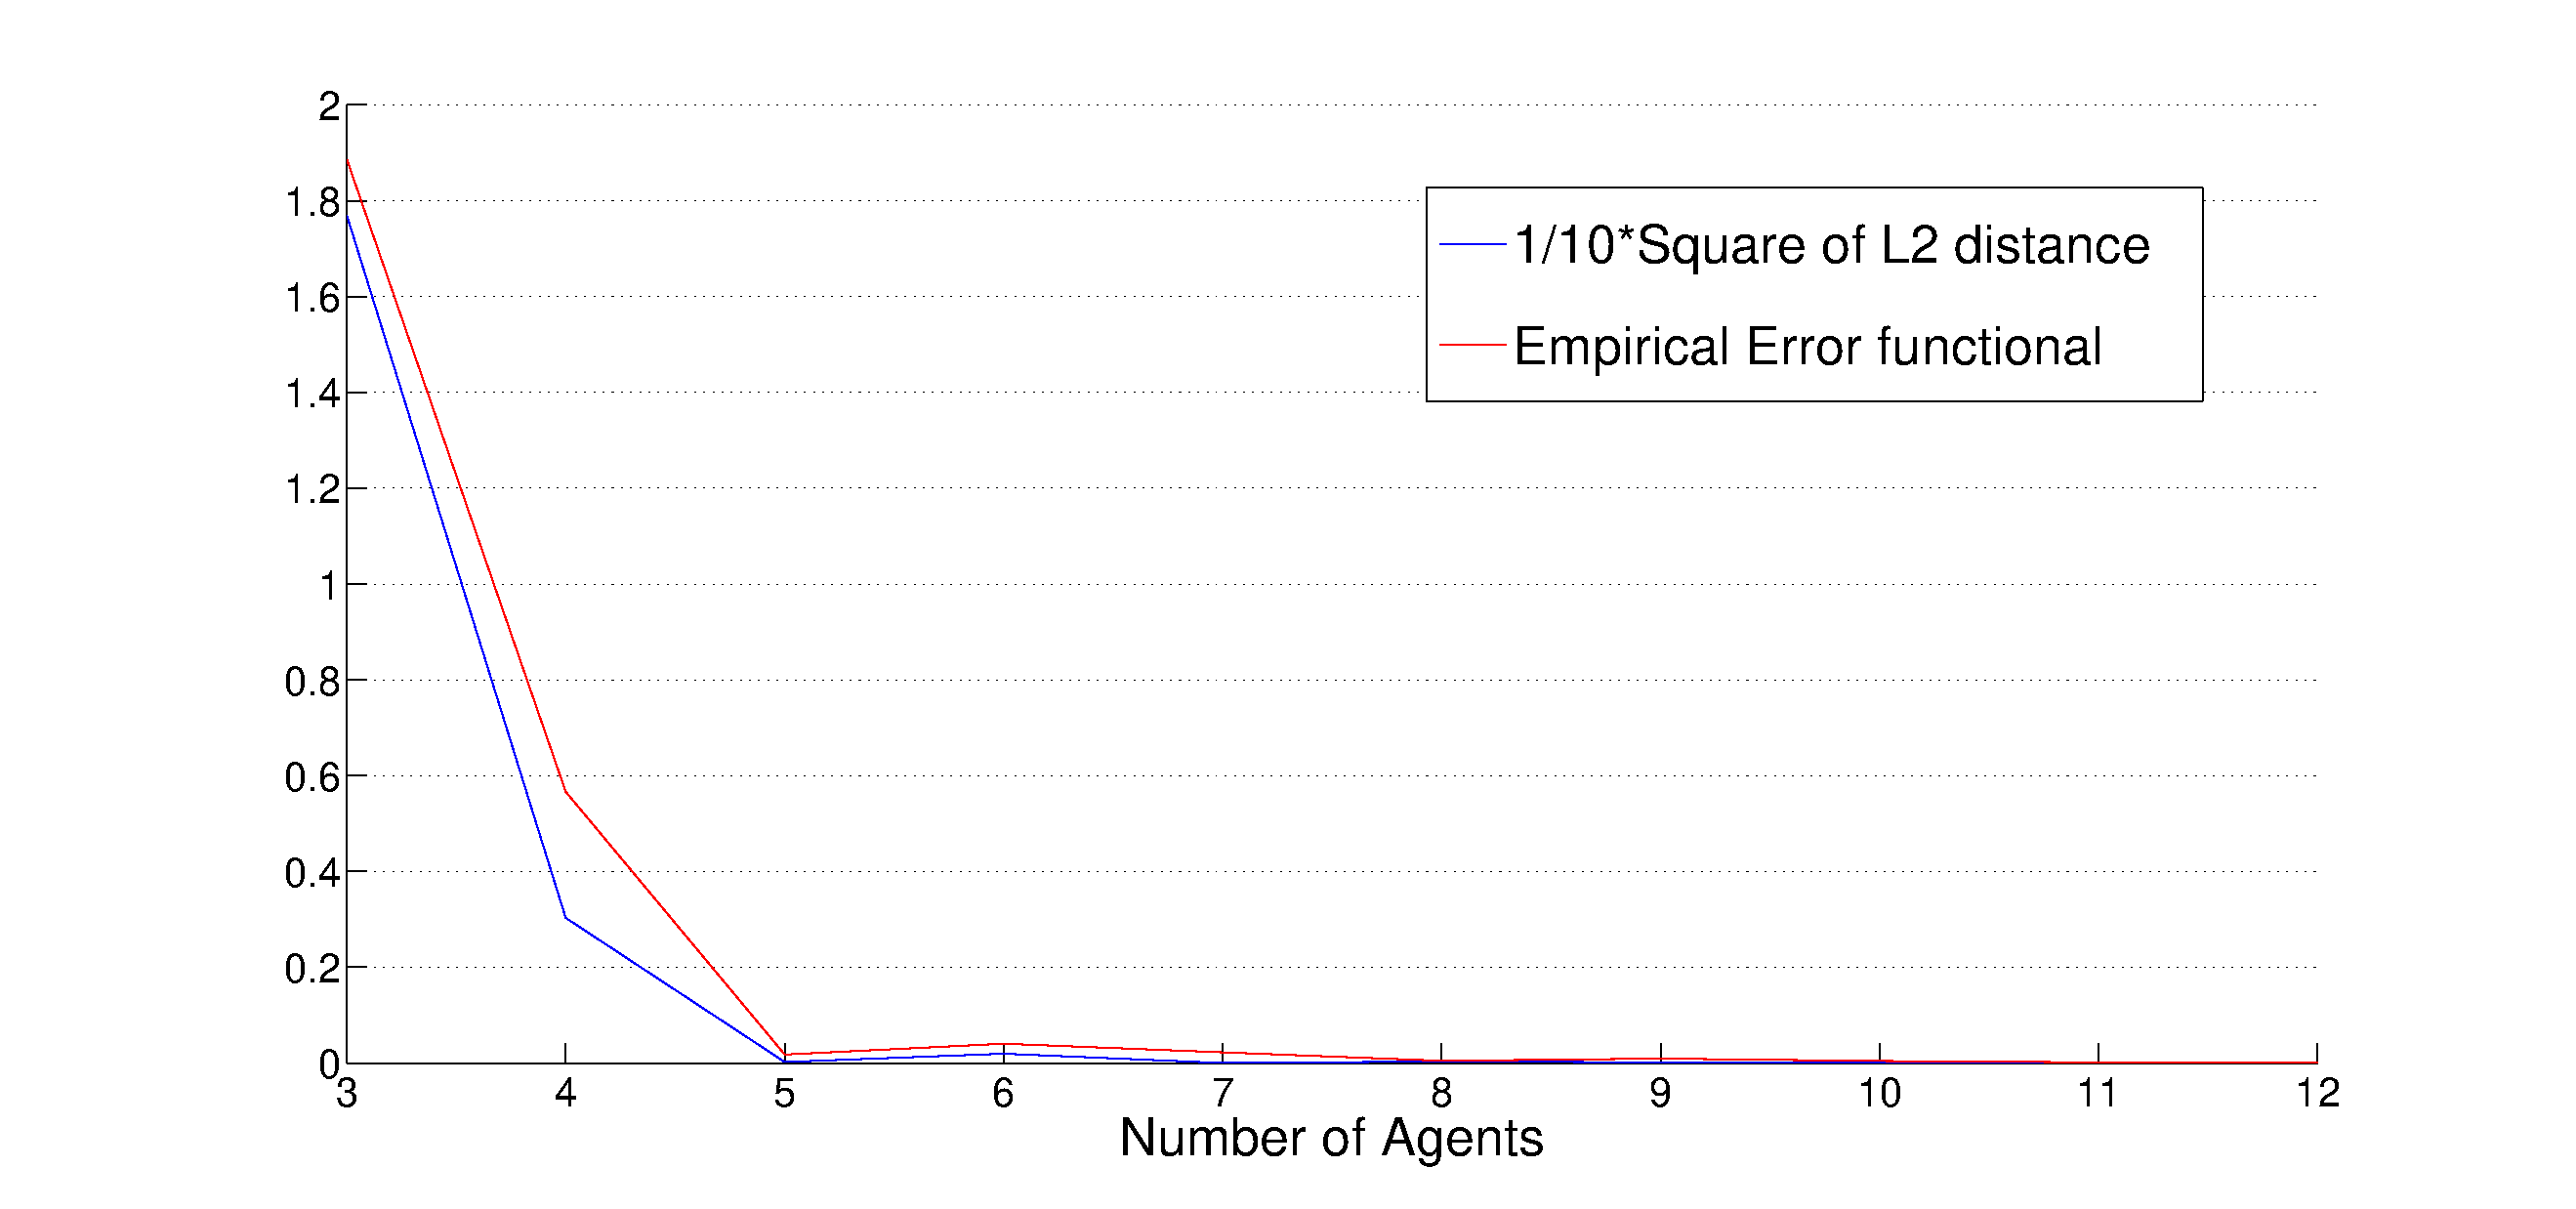
\includegraphics[width=1\textwidth]{Figures/figErrorN.eps}
%\end{center}
%\justifying
%\footnotesize{
%Plot of $\frac{1}{10}\|a-\widehat{a}_N\|^2_{L_2(\R_+,\rho)}$ and $\overline{\mathcal{E}}_N(\widehat{a}_N)$. We can estimate the constant $c_T$ with the value $\frac{1}{10}$.
%\begin{table}[h]
%\begin{center}
%\begin{tabular}{ |c|c|c|c|c|c| }
%\hline
%  $d$ & $T$ & $M$ & $N$ & $D(N)$ \\
%\hline
%\hline
%  $2$ & $0.5$ & $100$ & $[3,4,\ldots,12]$ & $3N-5$ \\
%\hline
%\end{tabular}
%\end{center}
%\end{table}}
%\end{minipage}
%\hspace{0.3cm}
%\begin{minipage}{0.49\textwidth}
%\begin{center}
%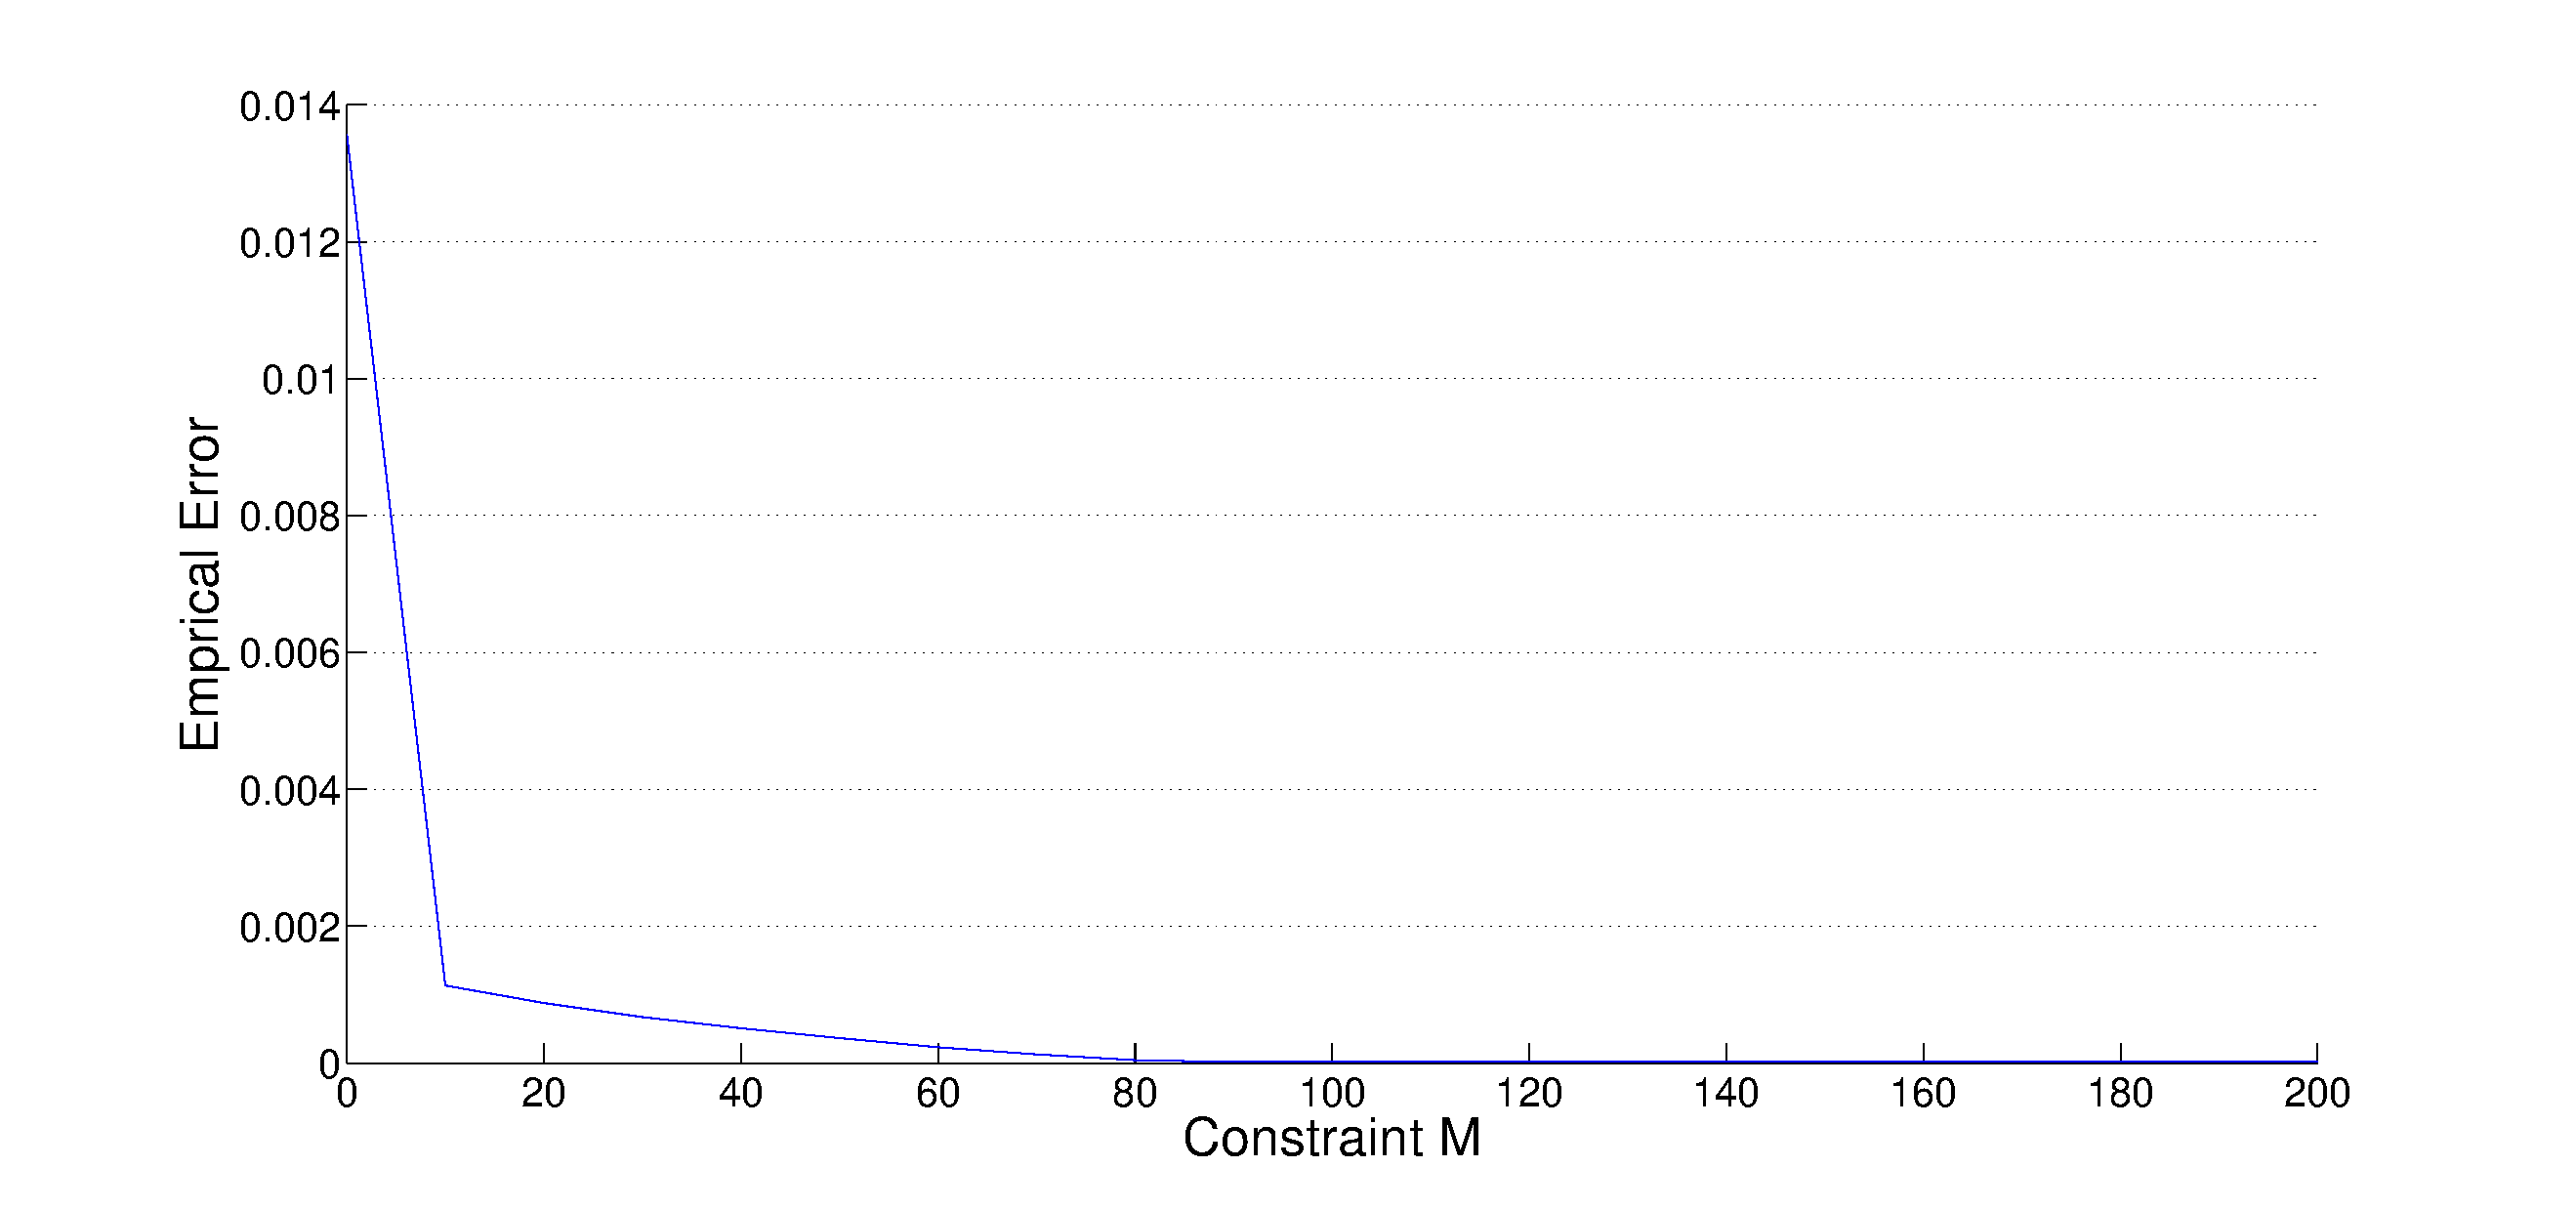
\includegraphics[width=1\textwidth]{Figures/figM.eps}
%\end{center}
%\footnotesize{
%\begin{table}[h]
%\begin{center}
%\begin{tabular}{ |c|c|c|c|c|c| }
%\hline
%  $d$ & $T$ & $M$ & $N$ & $D(N)$ \\
%\hline
%\hline
%  $2$ & $0.5$ & $[0,10,\ldots,200]$ & $50$ & $100$ \\
%\hline
%\end{tabular}
%\end{center}
%\end{table}}
%\end{minipage}
%\end{figure}
%}

\frame{
\frametitle{The coercivity condition}
\vspace{-0.2cm}
\begin{figure}[h]
\justifying
\begin{center}
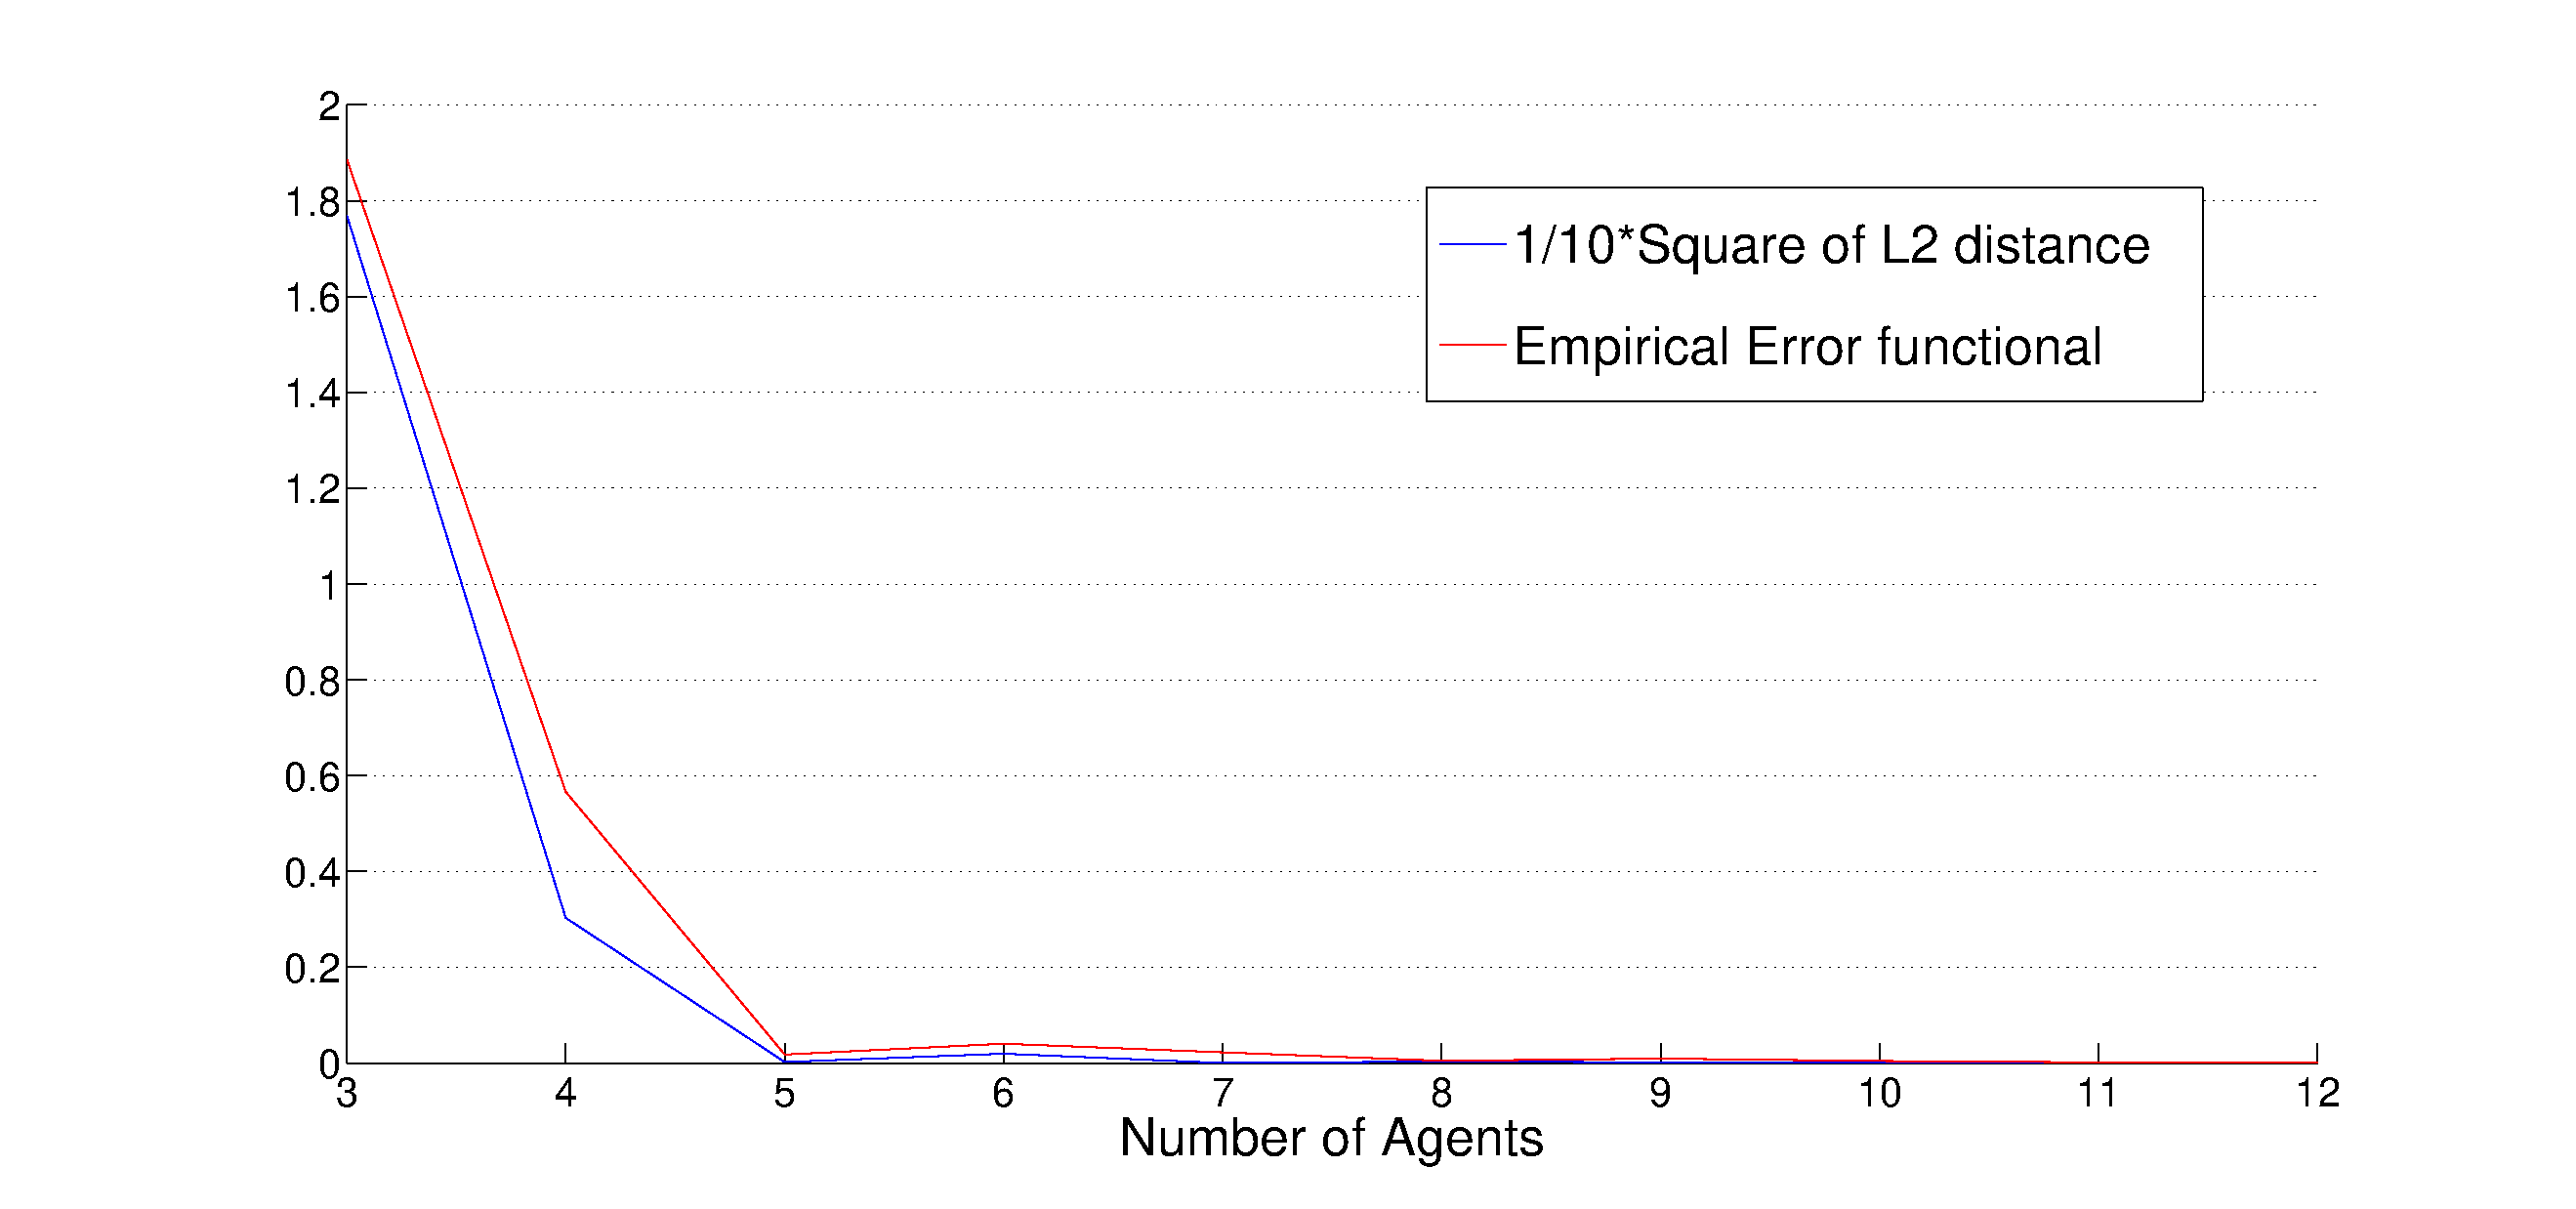
\includegraphics[width=0.9\textwidth]{Figures/figErrorN.eps}
\end{center}
\justifying
\footnotesize{
\caption{Plot of $\frac{1}{10}\|a-\widehat{a}_N\|^2_{L_2(\R_+,\rho)}$ and $\overline{\mathcal{E}}_N(\widehat{a}_N)$. We can estimate the constant $c_T$ with the value $\frac{1}{10}$.}
\begin{table}[h]
\begin{center}
\begin{tabular}{ |c|c|c|c|c|c| }
\hline
  $d$ & $T$ & $M$ & $N$ & $D(N)$ \\
\hline
\hline
  $2$ & $0.5$ & $100$ & $[3,4,\ldots,12]$ & $3N-5$ \\
\hline
\end{tabular}
\end{center}
\end{table}}
\end{figure}
}


\frame{
\frametitle{Tuning the constraint $M$ - I}
\justifying
{\color{blue}Left}: reconstruction of a kernel with different $M$.

{\color{blue}Right}: reconstruction of agents' trajectories with different $M$.

{\color{red}In white}: true kernel and true trajectories.

{\color{blue}The brighter the reconstruction, the bigger $M$.}
\begin{columns}
\hspace{-0.5cm}
\begin{column}{8cm}
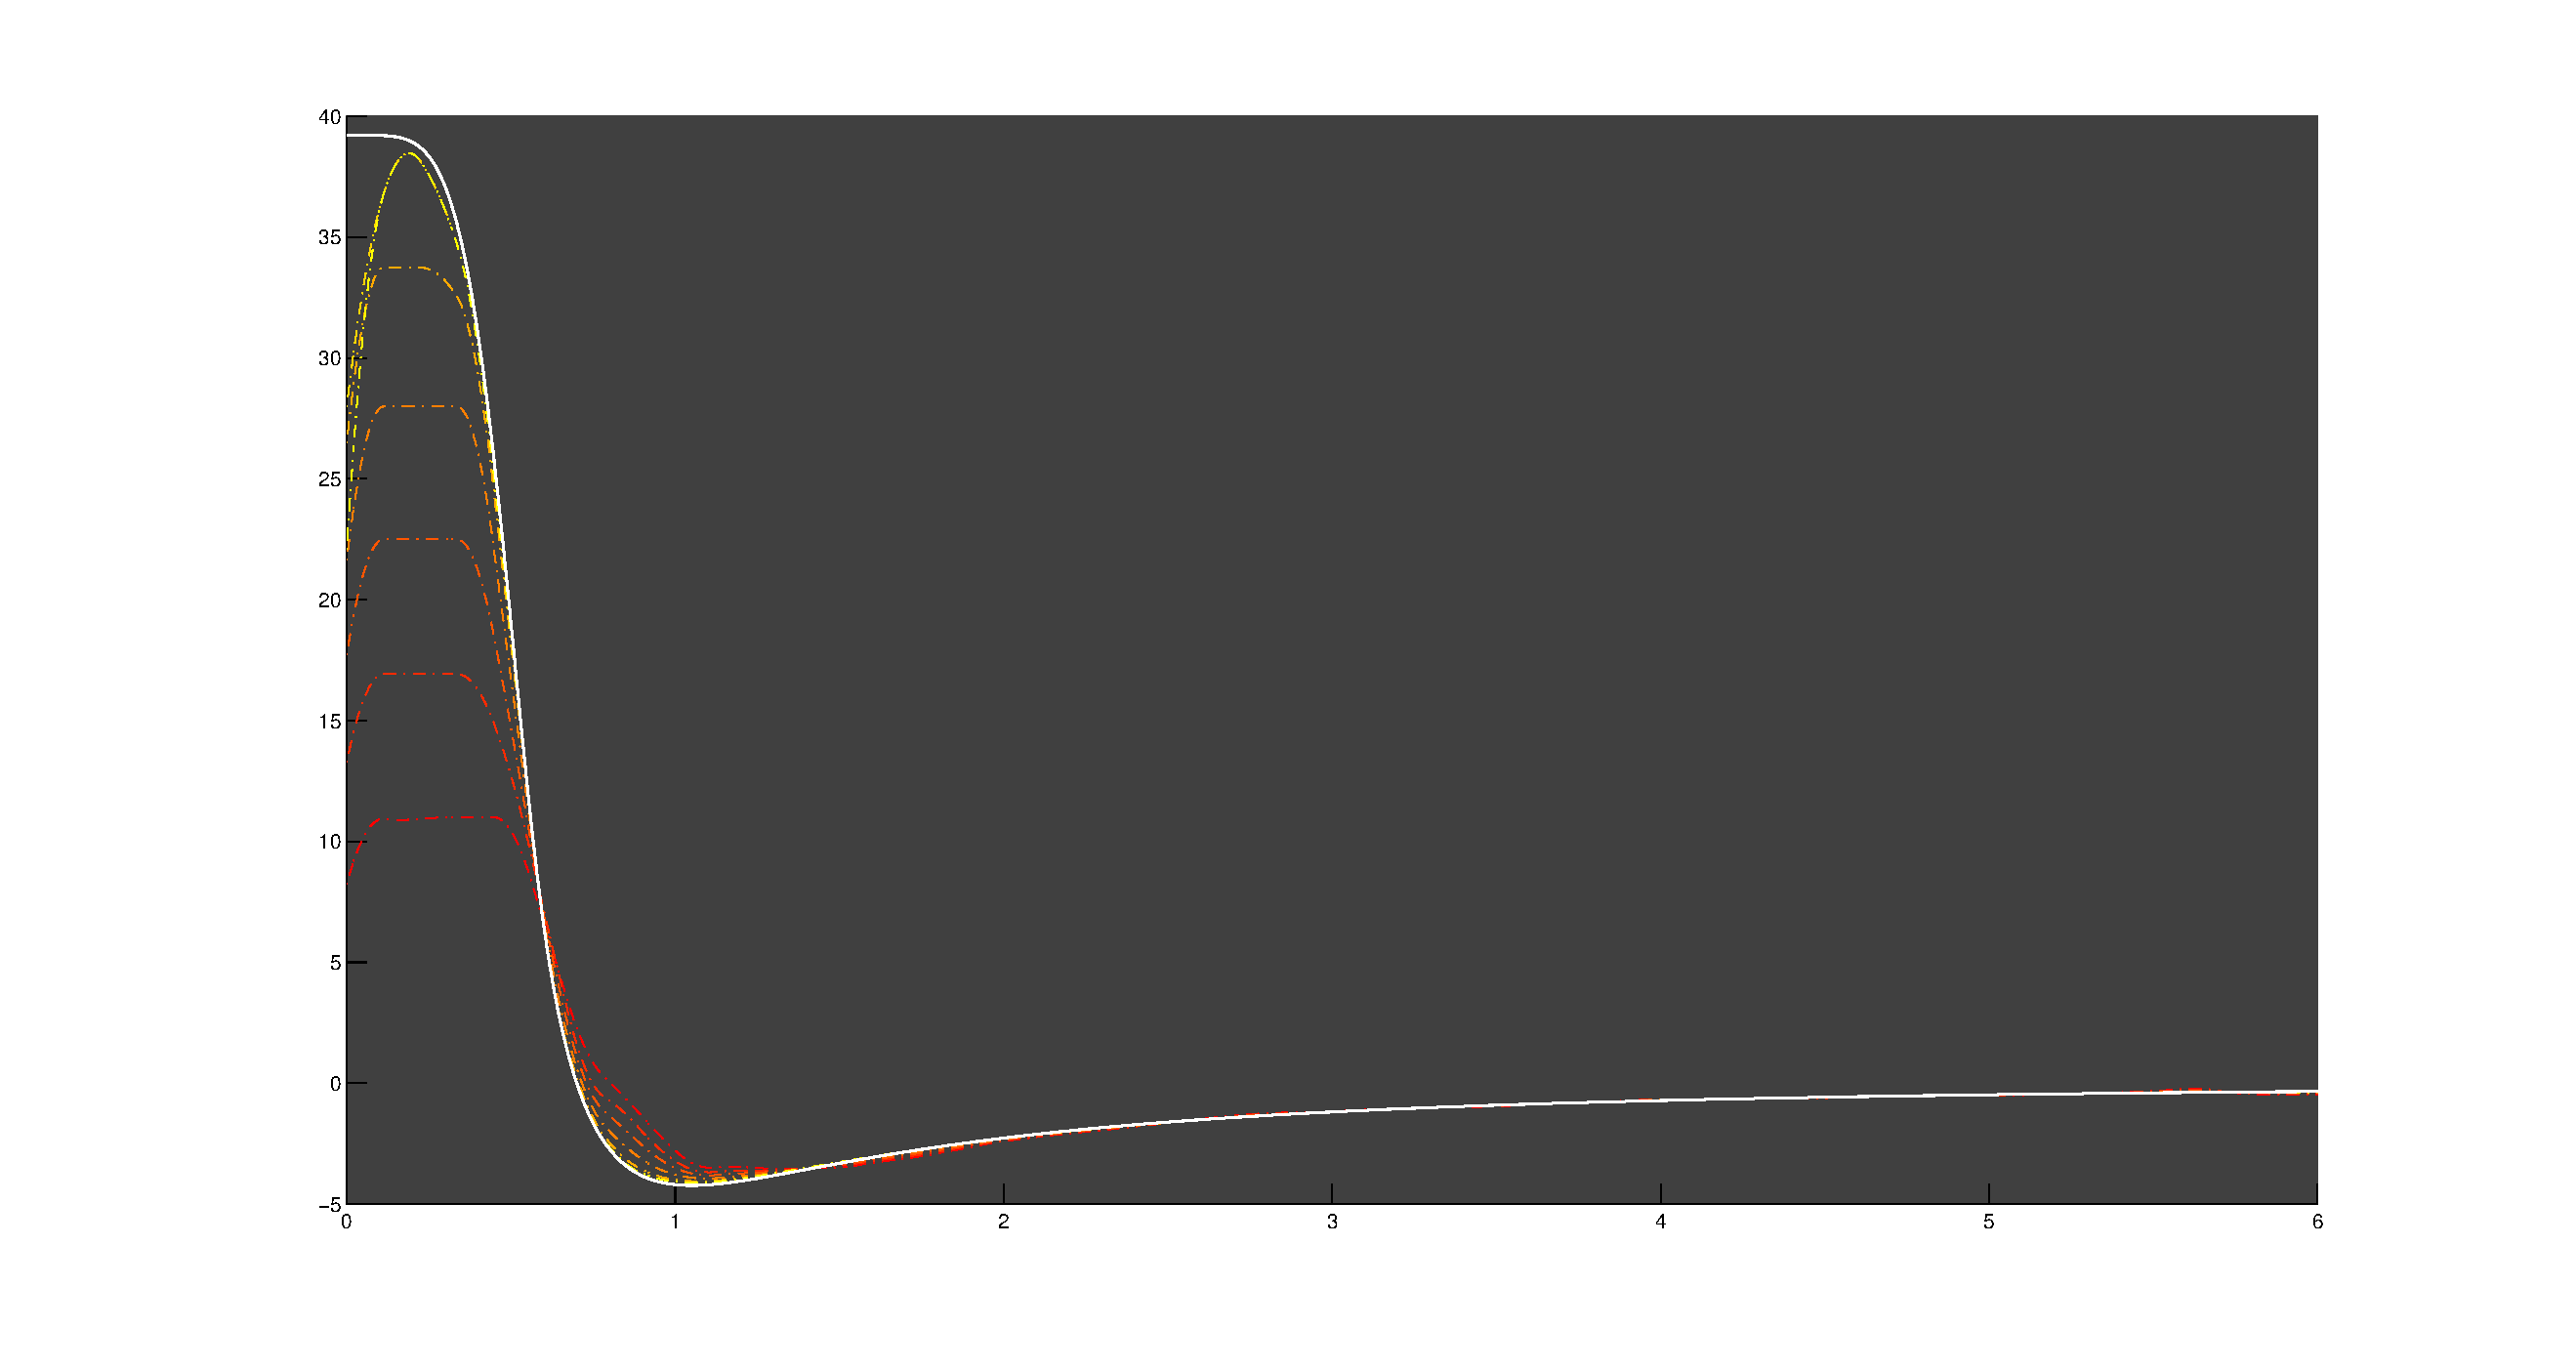
\includegraphics[width=1\textwidth]{Figures/figPotfun8}
\end{column}
\hspace{-0.9cm}
\begin{column}{5.5cm}
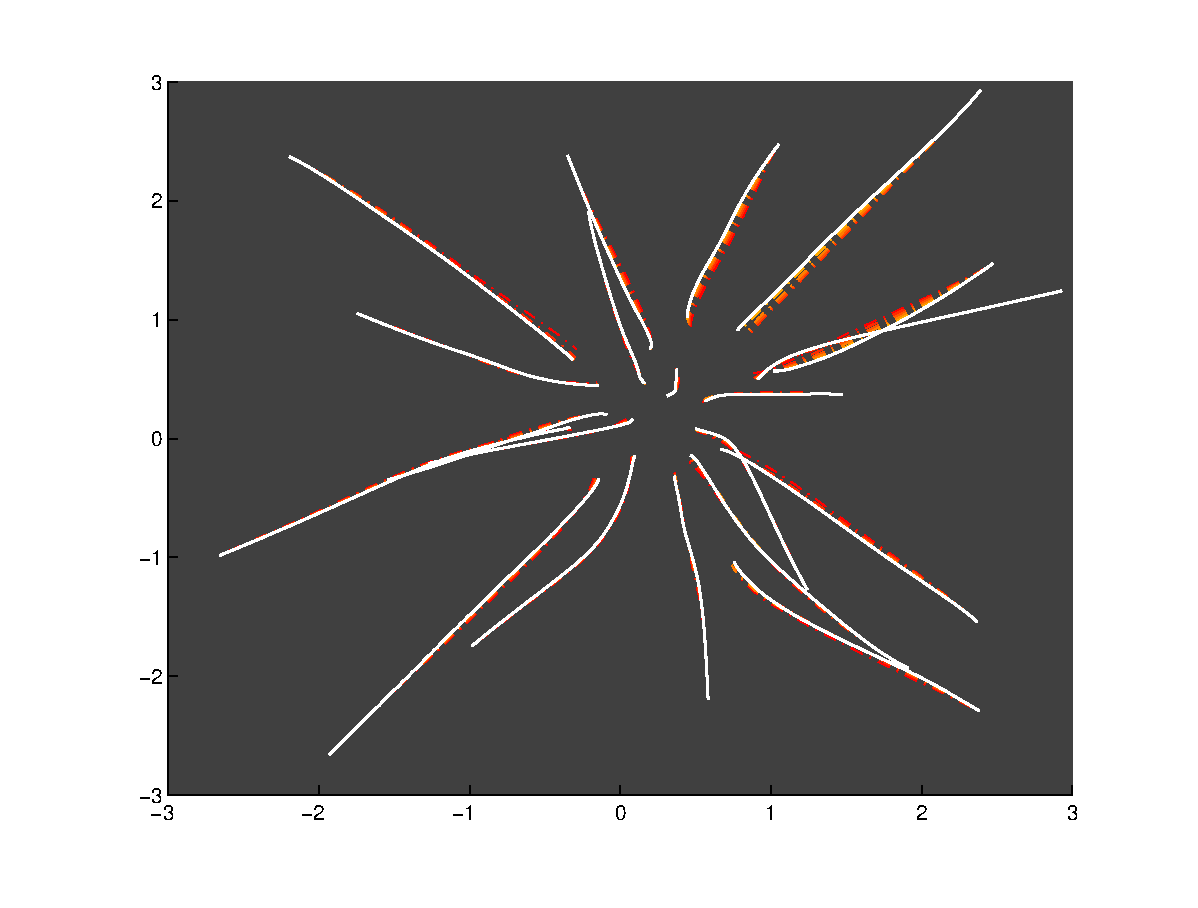
\includegraphics[width=1\textwidth]{Figures/figTrajfun8}
\end{column}
\end{columns}
\vspace{-0.1cm}
\footnotesize{\begin{table}[h]
\begin{center}
\begin{tabular}{ |c|c|c|c|c|c|c| }
\hline
 $d$ & $L$ & $T$ & $M$ & $N$ & $D(N)$ \\
\hline
\hline
$2$ & $3$ & $1$ & $2.7 \times [10,15,\ldots,40]$ & $20$ & $60$ \\
\hline
\end{tabular}
\end{center}
\end{table}}
}

\frame{
\frametitle{Tuning the constraint $M$ - II}
\justifying
{\color{blue}Left}: reconstruction of a kernel with different $M$.

{\color{blue}Right}: reconstruction of agents' trajectories with different $M$.

{\color{red}In white}: true kernel and true trajectories.

{\color{blue}The brighter the reconstruction, the bigger $M$.}
\begin{columns}
\hspace{-0.5cm}
\begin{column}{8cm}
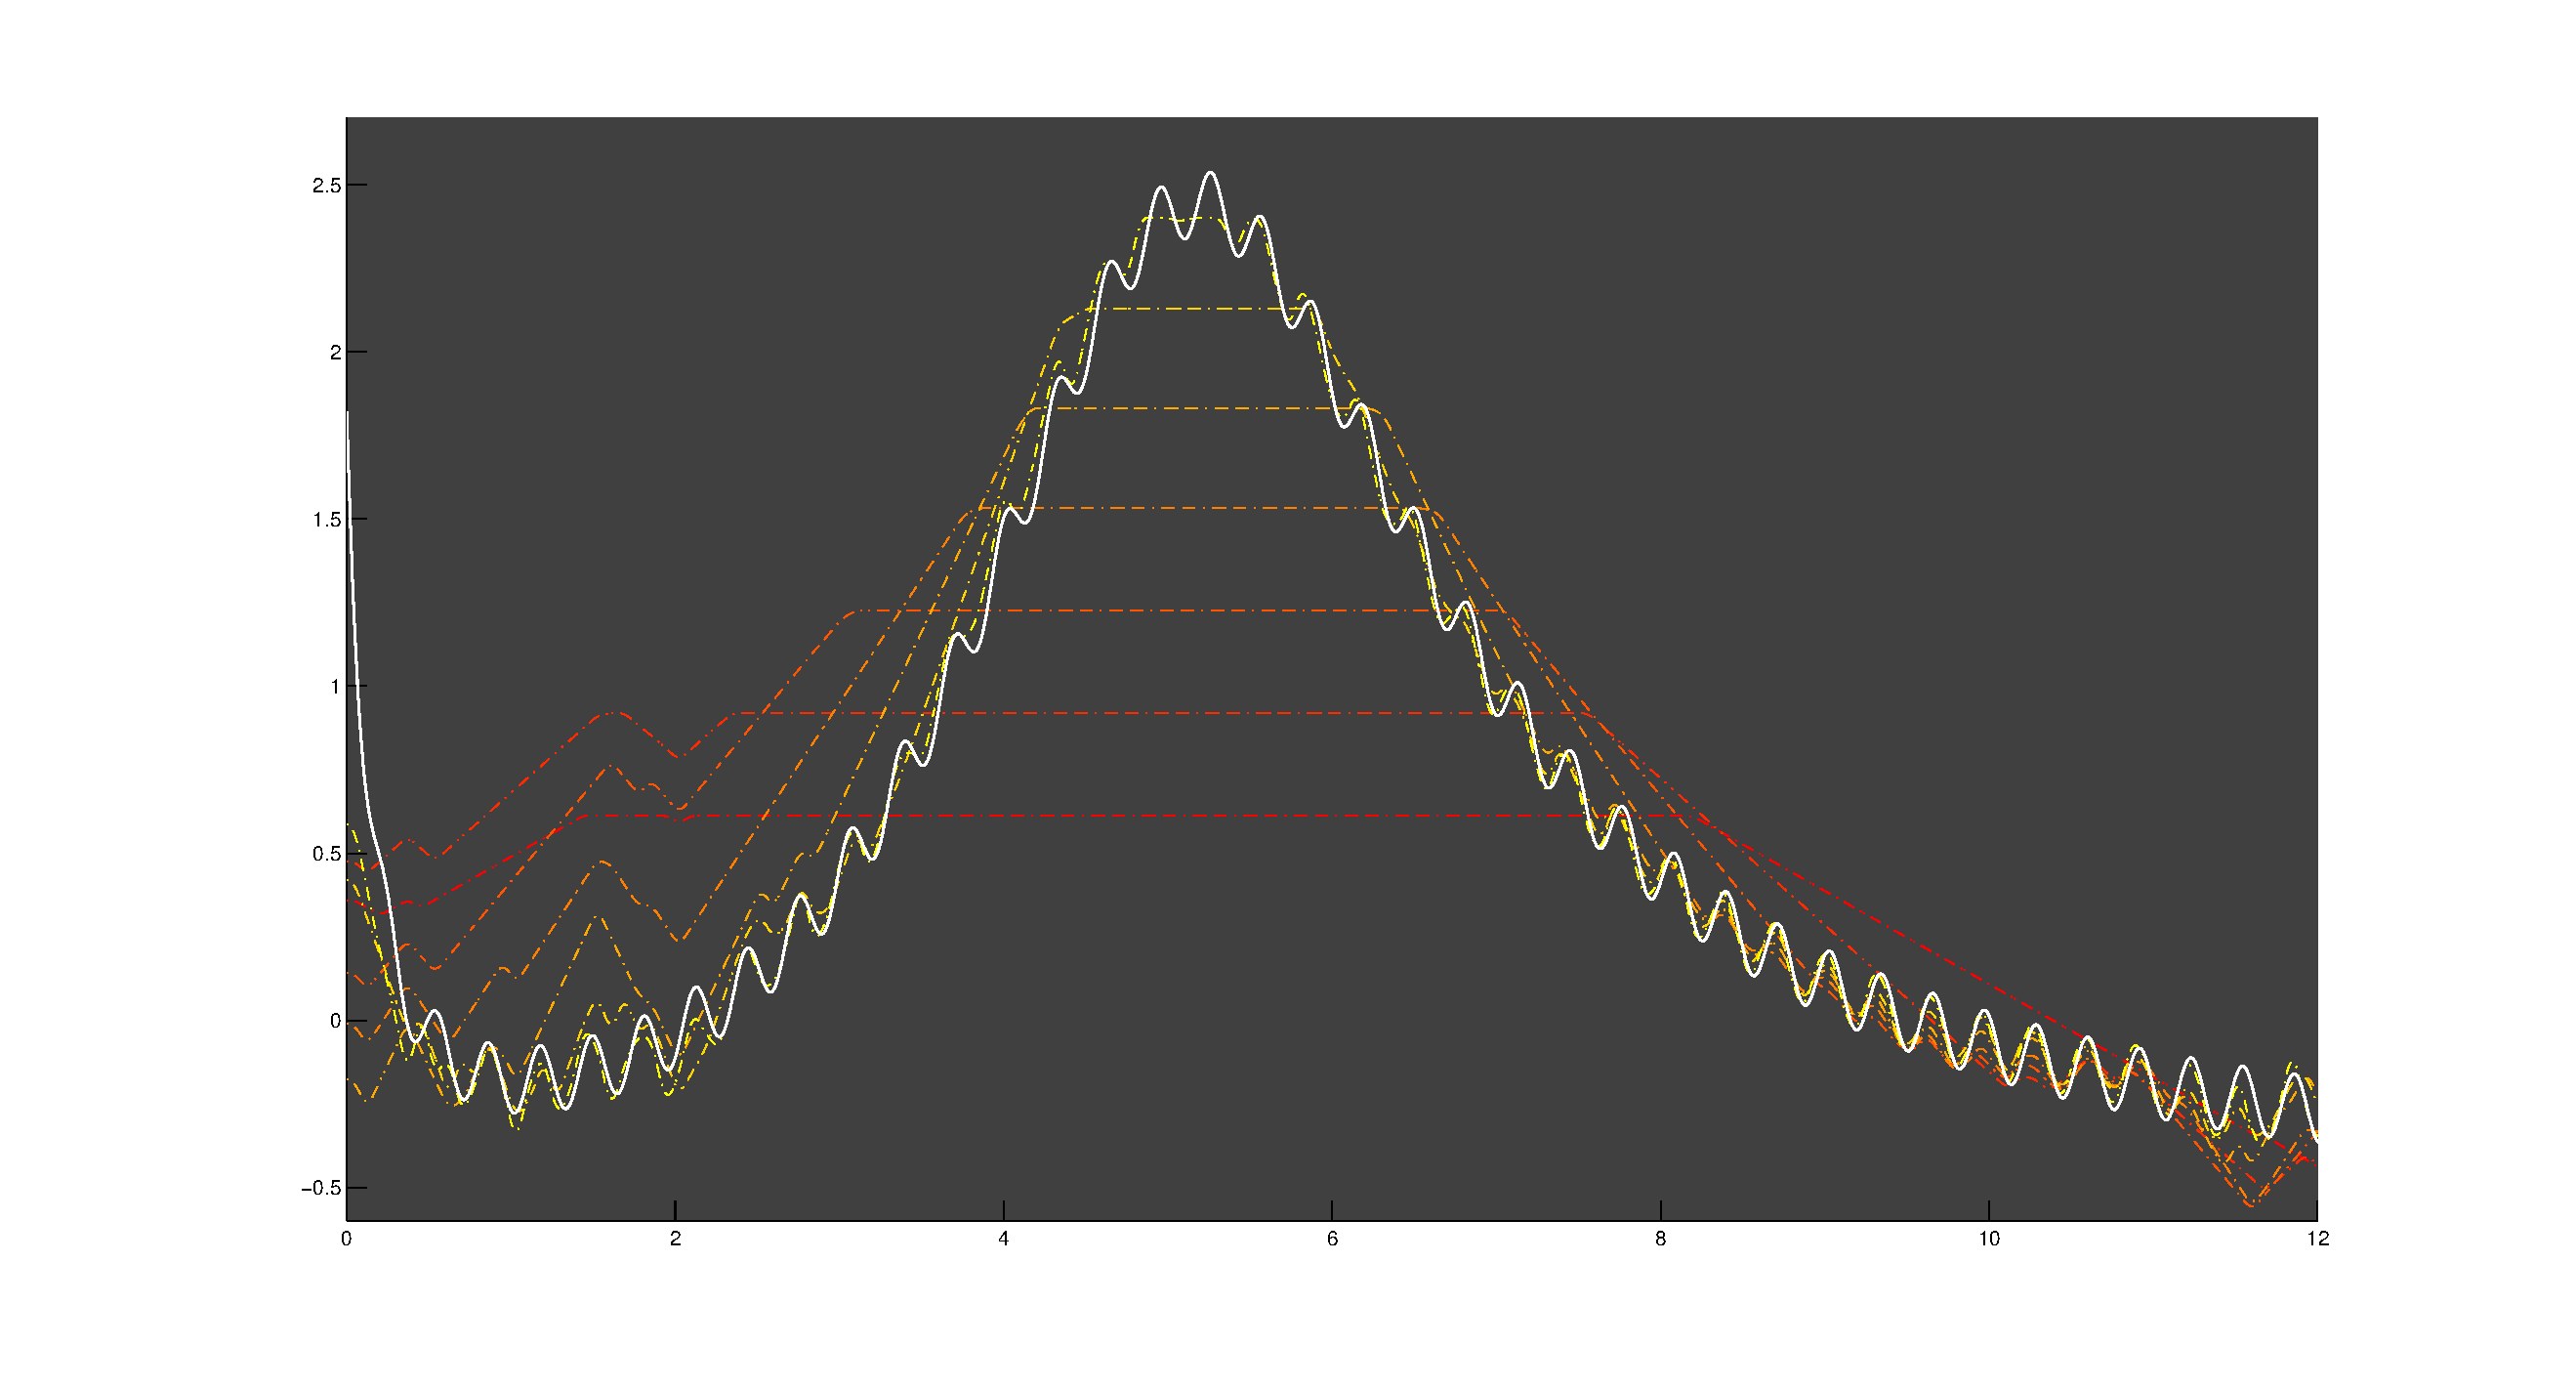
\includegraphics[width=1\textwidth]{Figures/figPotfun61}
\end{column}
\hspace{-0.9cm}
\begin{column}{5.5cm}
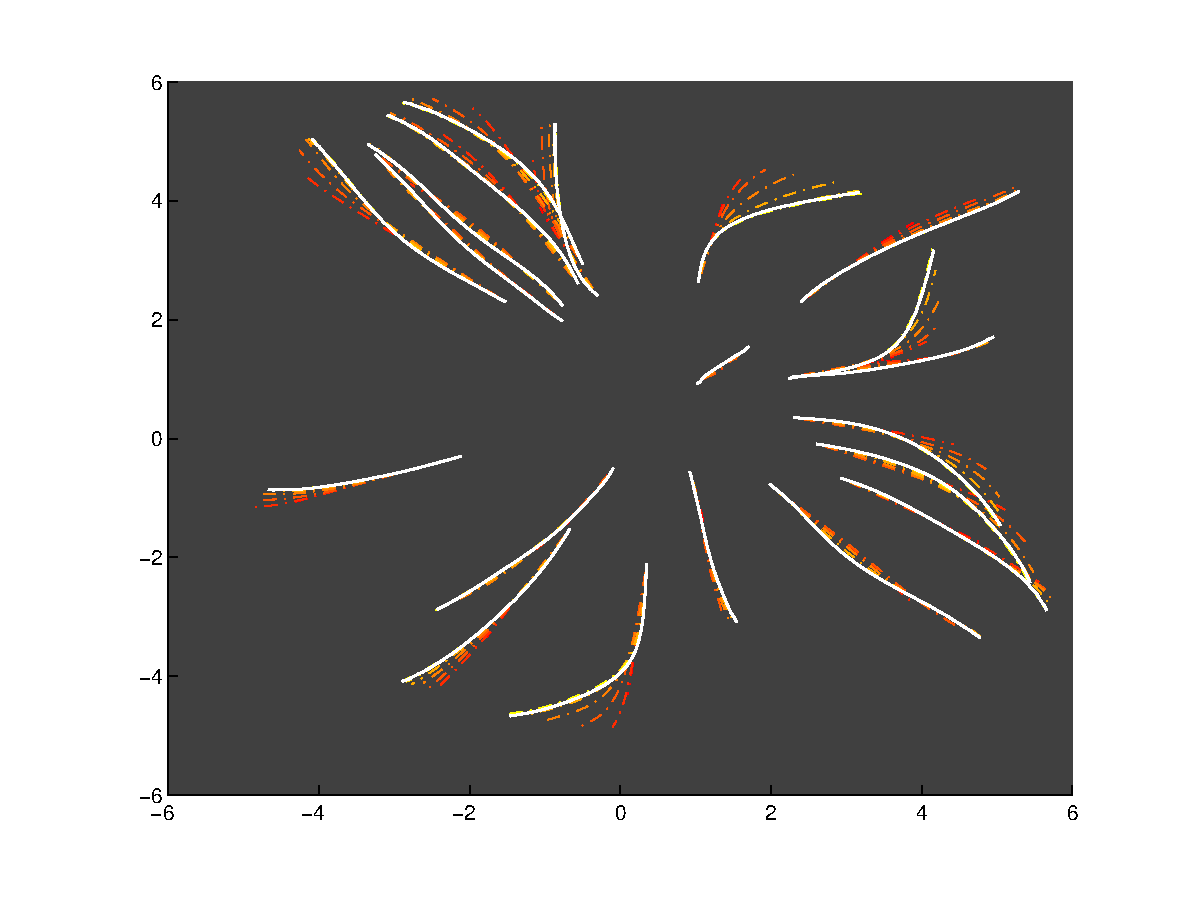
\includegraphics[width=1\textwidth]{Figures/figTrajfun61}
\end{column}
\end{columns}
\vspace{-0.1cm}
\footnotesize{\begin{table}[h]
\begin{center}
\begin{tabular}{ |c|c|c|c|c|c|c| }
\hline
 $d$ & $L$ & $T$ & $M$ & $N$ & $D(N)$ \\
\hline
\hline
$2$ & $3$ & $1$ & $1.25 \times [10,15,\ldots,40]$ & $20$ & $150$ \\
\hline
\end{tabular}
\end{center}
\end{table}}
}

\frame{
\frametitle{A few info}
\justifying
\begin{itemize}
\item {\bf \bnew WWW:} http://www-m15.ma.tum.de/Allgemeines/MattiaBongini 
\vspace{-0.1cm}
\item {\bf \bnew References}:
\begin{itemize}
\item {\color{blue}M. Bongini, M. Fornasier, M. Hansen, and M. Maggioni. \textit{Inferring interaction rules from observations of evolutive systems I: The variational approach.} in preparation, 2016.}
\item M. Bongini, M. Fornasier, M. Hansen, and M. Maggioni. \textit{Inferring interaction rules from observations of evolutive systems II: The universal learning approach.} in preparation, 2016.
\item G. Albi, M. Bongini, E. Cristiani, D. Kalise, \textit{Invisible Control of Self-Organizing Agents Leaving Unknown Environments}, submitted, 2015.
\item M. Bongini, M. Fornasier, F. Rossi, and F. Solombrino, \textit{Mean-Field Pontryagin Maximum Principle}, submitted, 2015.
\end{itemize}
\end{itemize}
}

%\frame{
%	\frametitle{Outlook: A second approach}
%	
%	\justifying
%	
%	We are currently investigating a second approach via random (discrete) $L_2$-projections: Equip $L_2(\rho)$ with a scalar
%	product
%	$$\langle f,g\rangle
%		=\frac{1}{T}\int_0^T\int_{\R^d}\bigl(F^{[f]}\ast\mu(t)\bigr)(x)\bullet\bigl(F^{[g]}\ast\mu(t)\bigr)(x)\,d\mu(t)(x)\,dt.$$
%	
%	\pause
%	
%	The coercivity condition now ensures that this is indeed a scalar product, and
%	$$\mathcal{E}^{[a]}(\widehat a)=\langle a-\widehat a,a-\widehat a\rangle\equiv\|a-\widehat a\|_\mu.$$
%	
%	\pause
%	
%	Minimizing $\mathcal{E}^{[a]}$ over (closed or finite dimensional) subspaces thus is equivalent to orthogonally projecting
%	onto that subspace w.r.t. $\langle\cdot,\cdot,\rangle$.
%}
%
%\frame{
%	\frametitle{A second approach - II}
%	
%	\justifying
%	
%	This is applied to subspaces $V_\Lambda$ of continuous polynomial spline functions w.r.t. a partition $\Lambda$ (particularly
%	piecewise constant and piecewise linear functions).
%	
%	\pause\vspace{3mm}
%	
%	Idea: Use an adaptive algorithm to generate the partitions
%	
%	\pause\vspace{3mm}
%	
%	Main problem (technical difficulty): The scalar product is non-local, i.e. functions with disjoint support are not automatically
%	orthogonal.
%}

\end{document}

